% Options for packages loaded elsewhere
\PassOptionsToPackage{unicode}{hyperref}
\PassOptionsToPackage{hyphens}{url}
\PassOptionsToPackage{dvipsnames,svgnames,x11names}{xcolor}
%
\documentclass[
  10pt,
  a4paper,
  german]{article}

\usepackage{amsmath,amssymb}
\usepackage{iftex}
\ifPDFTeX
  \usepackage[T1]{fontenc}
  \usepackage[utf8]{inputenc}
  \usepackage{textcomp} % provide euro and other symbols
\else % if luatex or xetex
  \usepackage{unicode-math}
  \defaultfontfeatures{Scale=MatchLowercase}
  \defaultfontfeatures[\rmfamily]{Ligatures=TeX,Scale=1}
\fi
\usepackage{lmodern}
\ifPDFTeX\else  
    % xetex/luatex font selection
\fi
% Use upquote if available, for straight quotes in verbatim environments
\IfFileExists{upquote.sty}{\usepackage{upquote}}{}
\IfFileExists{microtype.sty}{% use microtype if available
  \usepackage[]{microtype}
  \UseMicrotypeSet[protrusion]{basicmath} % disable protrusion for tt fonts
}{}
\makeatletter
\@ifundefined{KOMAClassName}{% if non-KOMA class
  \IfFileExists{parskip.sty}{%
    \usepackage{parskip}
  }{% else
    \setlength{\parindent}{0pt}
    \setlength{\parskip}{6pt plus 2pt minus 1pt}}
}{% if KOMA class
  \KOMAoptions{parskip=half}}
\makeatother
\usepackage{xcolor}
\usepackage[top=25mm,bottom=25mm,left=25mm,right=25mm]{geometry}
\usepackage{soul}
\setlength{\emergencystretch}{3em} % prevent overfull lines
\setcounter{secnumdepth}{3}
% Make \paragraph and \subparagraph free-standing
\ifx\paragraph\undefined\else
  \let\oldparagraph\paragraph
  \renewcommand{\paragraph}[1]{\oldparagraph{#1}\mbox{}}
\fi
\ifx\subparagraph\undefined\else
  \let\oldsubparagraph\subparagraph
  \renewcommand{\subparagraph}[1]{\oldsubparagraph{#1}\mbox{}}
\fi


\providecommand{\tightlist}{%
  \setlength{\itemsep}{0pt}\setlength{\parskip}{0pt}}\usepackage{longtable,booktabs,array}
\usepackage{calc} % for calculating minipage widths
% Correct order of tables after \paragraph or \subparagraph
\usepackage{etoolbox}
\makeatletter
\patchcmd\longtable{\par}{\if@noskipsec\mbox{}\fi\par}{}{}
\makeatother
% Allow footnotes in longtable head/foot
\IfFileExists{footnotehyper.sty}{\usepackage{footnotehyper}}{\usepackage{footnote}}
\makesavenoteenv{longtable}
\usepackage{graphicx}
\makeatletter
\def\maxwidth{\ifdim\Gin@nat@width>\linewidth\linewidth\else\Gin@nat@width\fi}
\def\maxheight{\ifdim\Gin@nat@height>\textheight\textheight\else\Gin@nat@height\fi}
\makeatother
% Scale images if necessary, so that they will not overflow the page
% margins by default, and it is still possible to overwrite the defaults
% using explicit options in \includegraphics[width, height, ...]{}
\setkeys{Gin}{width=\maxwidth,height=\maxheight,keepaspectratio}
% Set default figure placement to htbp
\makeatletter
\def\fps@figure{htbp}
\makeatother

\usepackage{amssymb, amsmath}
\numberwithin{equation}{section}

\usepackage[utf8]{inputenc}
\usepackage{lastpage} % counts all the pages, used in footer
\usepackage{hyperref}

% Flexible Multicolumn Option
\usepackage{multicol}
\setlength\columnsep{20pt}

% Package for enabling colors (colorful output)
\usepackage[dvipsnames]{xcolor}
\definecolor{darkgreen}{HTML}{014f32}

% Icons - http://mirrors.ctan.org/fonts/fontawesome5/doc/fontawesome5.pdf
\usepackage{fontawesome5}


\usepackage{tabularx}
\renewcommand\tabularxcolumn[1]{m{#1}} % vertically center content


\usepackage[nodisplayskipstretch]{setspace}

% Font Configuration
\usepackage{lmodern}
\renewcommand{\familydefault}{\sfdefault}
\usepackage{cmbright}
\usepackage[scaled=0.85]{beramono}

% 
\usepackage{fancyhdr}

\renewcommand{\headrulewidth}{1pt}
\renewcommand{\footrulewidth}{1pt}

\pagestyle{fancy}
\fancyhead{} % clear all header fields
\makeatletter
\fancyhead[R]{\@title}
\makeatother
\fancyhead[L]{HSLU T\&A}
\fancyfoot{} % clear all footer fields
\fancyfoot[C]{\thepage\ / \pageref{LastPage}}
\fancyfoot[R]{NRT}
\fancyfoot[L]{\today}

% introduces conditions environment to create nice equation parameter descriptions
\usepackage{array}

\newenvironment{conditions}
  {\par\vspace{\abovedisplayskip}\noindent\begin{tabular}{>{$}l<{$} @{${}:{}$} l}}
  {\end{tabular}\par\vspace{\belowdisplayskip}}

% Used for pandoc code block generations.
% Introduces breaklines for overflowing code blocks, by defining the Highlighting environment with breakline & symbol.
% Don't know what commandchars does :)
\usepackage{fvextra}
\DefineVerbatimEnvironment{Highlighting}{Verbatim}{
  breaklines,
  breaksymbolleft={\textcolor{gray}{\scriptsize\ensuremath\hookrightarrow}},
  commandchars=\\\{\}
}



\let\paragraph\oldparagraph
\let\subparagraph\oldsubparagraph

\usepackage{xhfill}
\usepackage[explicit]{titlesec}
\renewcommand{\paragraph}[1]{\oldparagraph{#1}\mbox{}\par}

\titleformat{\section}[block]{\bfseries\Large}{\thetitle.}{3mm}{#1\space\xrfill[0.6ex]{1pt}}
\makeatletter
\@ifpackageloaded{tcolorbox}{}{\usepackage[skins,breakable]{tcolorbox}}
\@ifpackageloaded{fontawesome5}{}{\usepackage{fontawesome5}}
\definecolor{quarto-callout-color}{HTML}{909090}
\definecolor{quarto-callout-note-color}{HTML}{0758E5}
\definecolor{quarto-callout-important-color}{HTML}{CC1914}
\definecolor{quarto-callout-warning-color}{HTML}{EB9113}
\definecolor{quarto-callout-tip-color}{HTML}{00A047}
\definecolor{quarto-callout-caution-color}{HTML}{FC5300}
\definecolor{quarto-callout-color-frame}{HTML}{acacac}
\definecolor{quarto-callout-note-color-frame}{HTML}{4582ec}
\definecolor{quarto-callout-important-color-frame}{HTML}{d9534f}
\definecolor{quarto-callout-warning-color-frame}{HTML}{f0ad4e}
\definecolor{quarto-callout-tip-color-frame}{HTML}{02b875}
\definecolor{quarto-callout-caution-color-frame}{HTML}{fd7e14}
\makeatother
\makeatletter
\makeatother
\makeatletter
\makeatother
\makeatletter
\@ifpackageloaded{caption}{}{\usepackage{caption}}
\AtBeginDocument{%
\ifdefined\contentsname
  \renewcommand*\contentsname{Inhaltsverzeichnis}
\else
  \newcommand\contentsname{Inhaltsverzeichnis}
\fi
\ifdefined\listfigurename
  \renewcommand*\listfigurename{Abbildungsverzeichnis}
\else
  \newcommand\listfigurename{Abbildungsverzeichnis}
\fi
\ifdefined\listtablename
  \renewcommand*\listtablename{Tabellenverzeichnis}
\else
  \newcommand\listtablename{Tabellenverzeichnis}
\fi
\ifdefined\figurename
  \renewcommand*\figurename{Abbildung}
\else
  \newcommand\figurename{Abbildung}
\fi
\ifdefined\tablename
  \renewcommand*\tablename{Tabelle}
\else
  \newcommand\tablename{Tabelle}
\fi
}
\@ifpackageloaded{float}{}{\usepackage{float}}
\floatstyle{ruled}
\@ifundefined{c@chapter}{\newfloat{codelisting}{h}{lop}}{\newfloat{codelisting}{h}{lop}[chapter]}
\floatname{codelisting}{Listing}
\newcommand*\listoflistings{\listof{codelisting}{Listingverzeichnis}}
\makeatother
\makeatletter
\@ifpackageloaded{caption}{}{\usepackage{caption}}
\@ifpackageloaded{subcaption}{}{\usepackage{subcaption}}
\makeatother
\makeatletter
\@ifpackageloaded{tcolorbox}{}{\usepackage[skins,breakable]{tcolorbox}}
\makeatother
\makeatletter
\@ifundefined{shadecolor}{\definecolor{shadecolor}{rgb}{.97, .97, .97}}
\makeatother
\makeatletter
\@ifundefined{codebgcolor}{\definecolor{codebgcolor}{HTML}{f7f7f7}}
\makeatother
\makeatletter
\makeatother
\ifLuaTeX
\usepackage[bidi=basic]{babel}
\else
\usepackage[bidi=default]{babel}
\fi
\babelprovide[main,import]{ngerman}
% get rid of language-specific shorthands (see #6817):
\let\LanguageShortHands\languageshorthands
\def\languageshorthands#1{}
\ifLuaTeX
  \usepackage{selnolig}  % disable illegal ligatures
\fi
\IfFileExists{bookmark.sty}{\usepackage{bookmark}}{\usepackage{hyperref}}
\IfFileExists{xurl.sty}{\usepackage{xurl}}{} % add URL line breaks if available
\urlstyle{same} % disable monospaced font for URLs
\hypersetup{
  pdftitle={Nachrichtentechnik},
  pdfauthor={Joel von Rotz \& Andreas Ming},
  pdflang={de},
  colorlinks=true,
  linkcolor={blue},
  filecolor={Maroon},
  citecolor={Blue},
  urlcolor={Blue},
  pdfcreator={LaTeX via pandoc}}

\title{Nachrichtentechnik}
\author{Joel von Rotz \& Andreas Ming}
\date{2023-03-30}

\begin{document}
 % [START] title
 % [ELSE] beamer

\makeatletter
\begin{center}
  \vspace*{0.5cm}
  
  \textbf{\Huge \@title} \\
  \vspace{0.1cm}
  \textsf{\normalsize Zusammenfassung}
  
  \vspace{0.1cm}

  {\Large {\@author}}
  
  \vspace{0.5cm}

\end{center}
\makeatother

 % [START] Source
\begin{center}
{\large \faGithub\space \href{https://github.com/joelvonrotz/bachelor-electrical-engineering/tree/main/semester\%204/summary/nachrichtentechnik}{Quelldateien}}
\end{center}
 % [END] title


 % [END] beamer
 % [END] title


\ifdefined\Shaded\renewenvironment{Shaded}{\begin{tcolorbox}[colback={shadecolor}, boxrule=0pt, frame hidden, enhanced, breakable]}{\end{tcolorbox}}\fi\ifdefined\Shaded\renewenvironment{Shaded}{\begin{tcolorbox}[boxrule=0pt, breakable, frame hidden, sharp corners, colback={codebgcolor}, borderline west={3pt}{0pt}{shadecolor}, enhanced]}{\end{tcolorbox}}\fi

\renewcommand*\contentsname{Inhaltsverzeichnis}
{
\hypersetup{linkcolor=}
\setcounter{tocdepth}{3}
\tableofcontents
}
\hypertarget{einfuxfchrung}{%
\section{Einführung}\label{einfuxfchrung}}

\hypertarget{struktur-von-kommunikationssystemen}{%
\subsection{Struktur von
Kommunikationssystemen}\label{struktur-von-kommunikationssystemen}}

\hypertarget{punkt-punkt-verbindung}{%
\subsubsection{Punkt-Punkt Verbindung}\label{punkt-punkt-verbindung}}

\begin{figure}[H]

{\centering 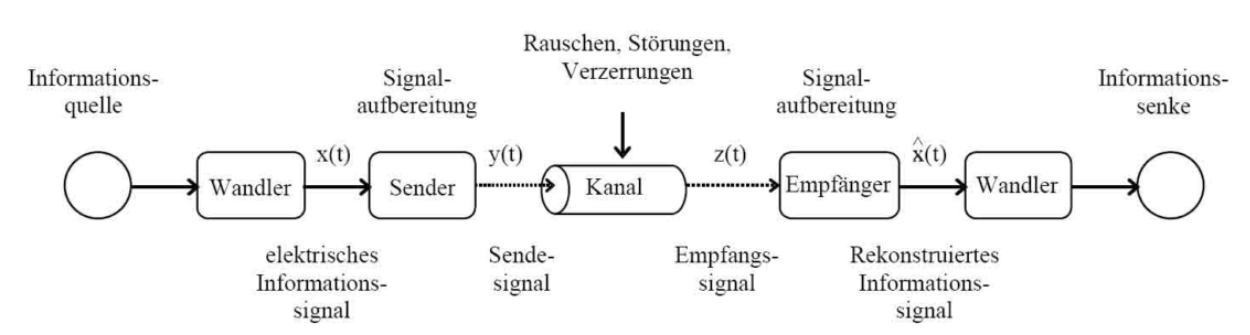
\includegraphics{images/01_PunktZuPunkt.png}

}

\caption{Funktionsblöcke einer Punkt-zu-Punkt-Verbindung}

\end{figure}

\begin{itemize}
\item
  \emph{Simplex-Verbindung}: Die Information fliesst nur von A nach B.
\item
  \emph{Halbduplex-Verbindung}: Es kann nur die eine oder andere Seite
  Informationen senden.
\item
  \emph{Vollduplex-Verbindung}: Informationen können einander unabhängig
  voneinander übermittelt werden.
\end{itemize}

\begin{figure}[H]

{\centering 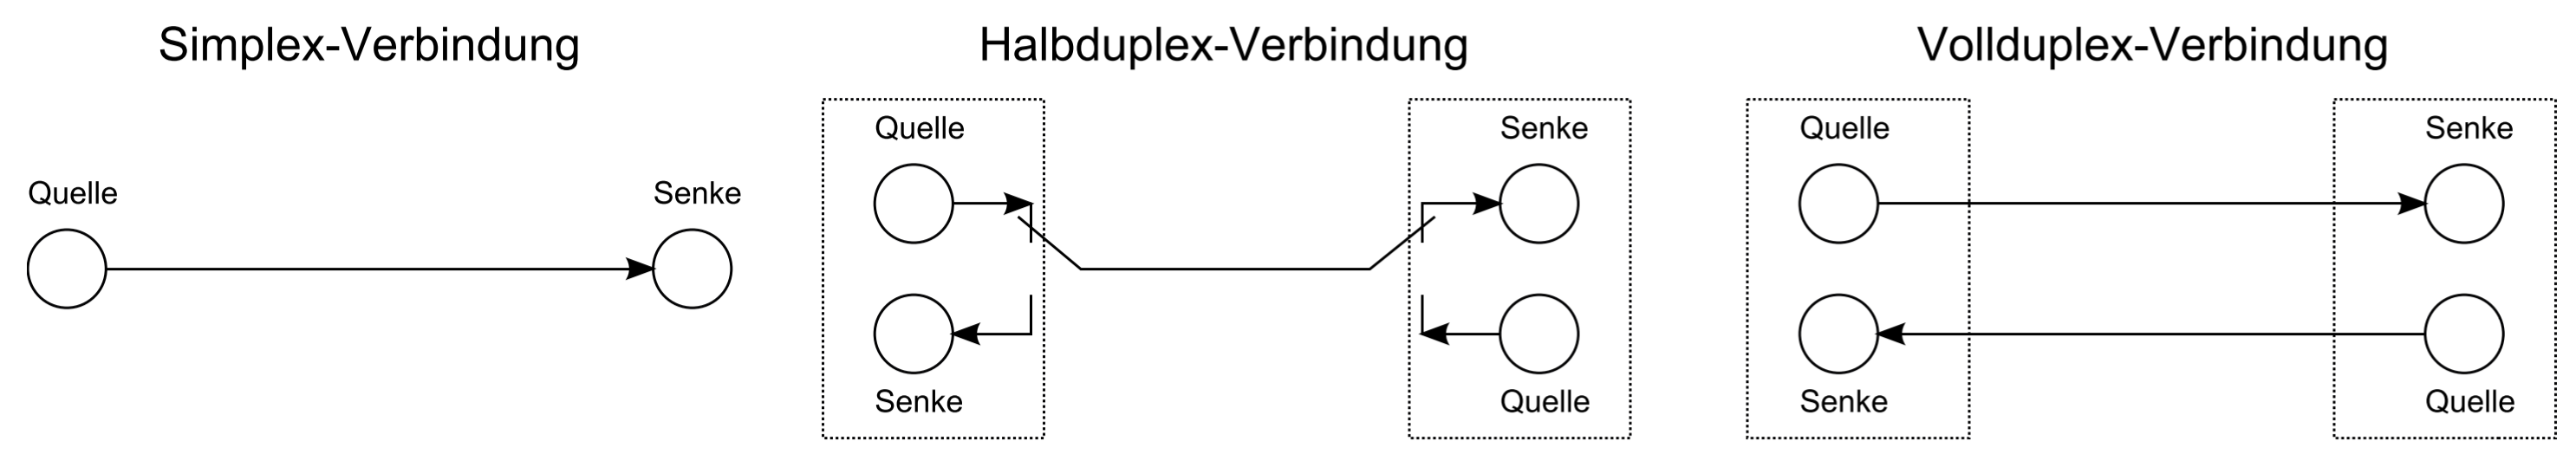
\includegraphics{images/01_Verbindungsarten.png}

}

\caption{Mögliche Verbindungsarten}

\end{figure}

\hypertarget{kommunikationsnetz}{%
\subsubsection{Kommunikationsnetz}\label{kommunikationsnetz}}

Durch Zusammenführen mehrerer Grundelemente entsteht ein
Kommunikationsnetz, an das eine Vielzahl von Teilnehmern angeschlossen
werden können.

\begin{figure}[H]

{\centering 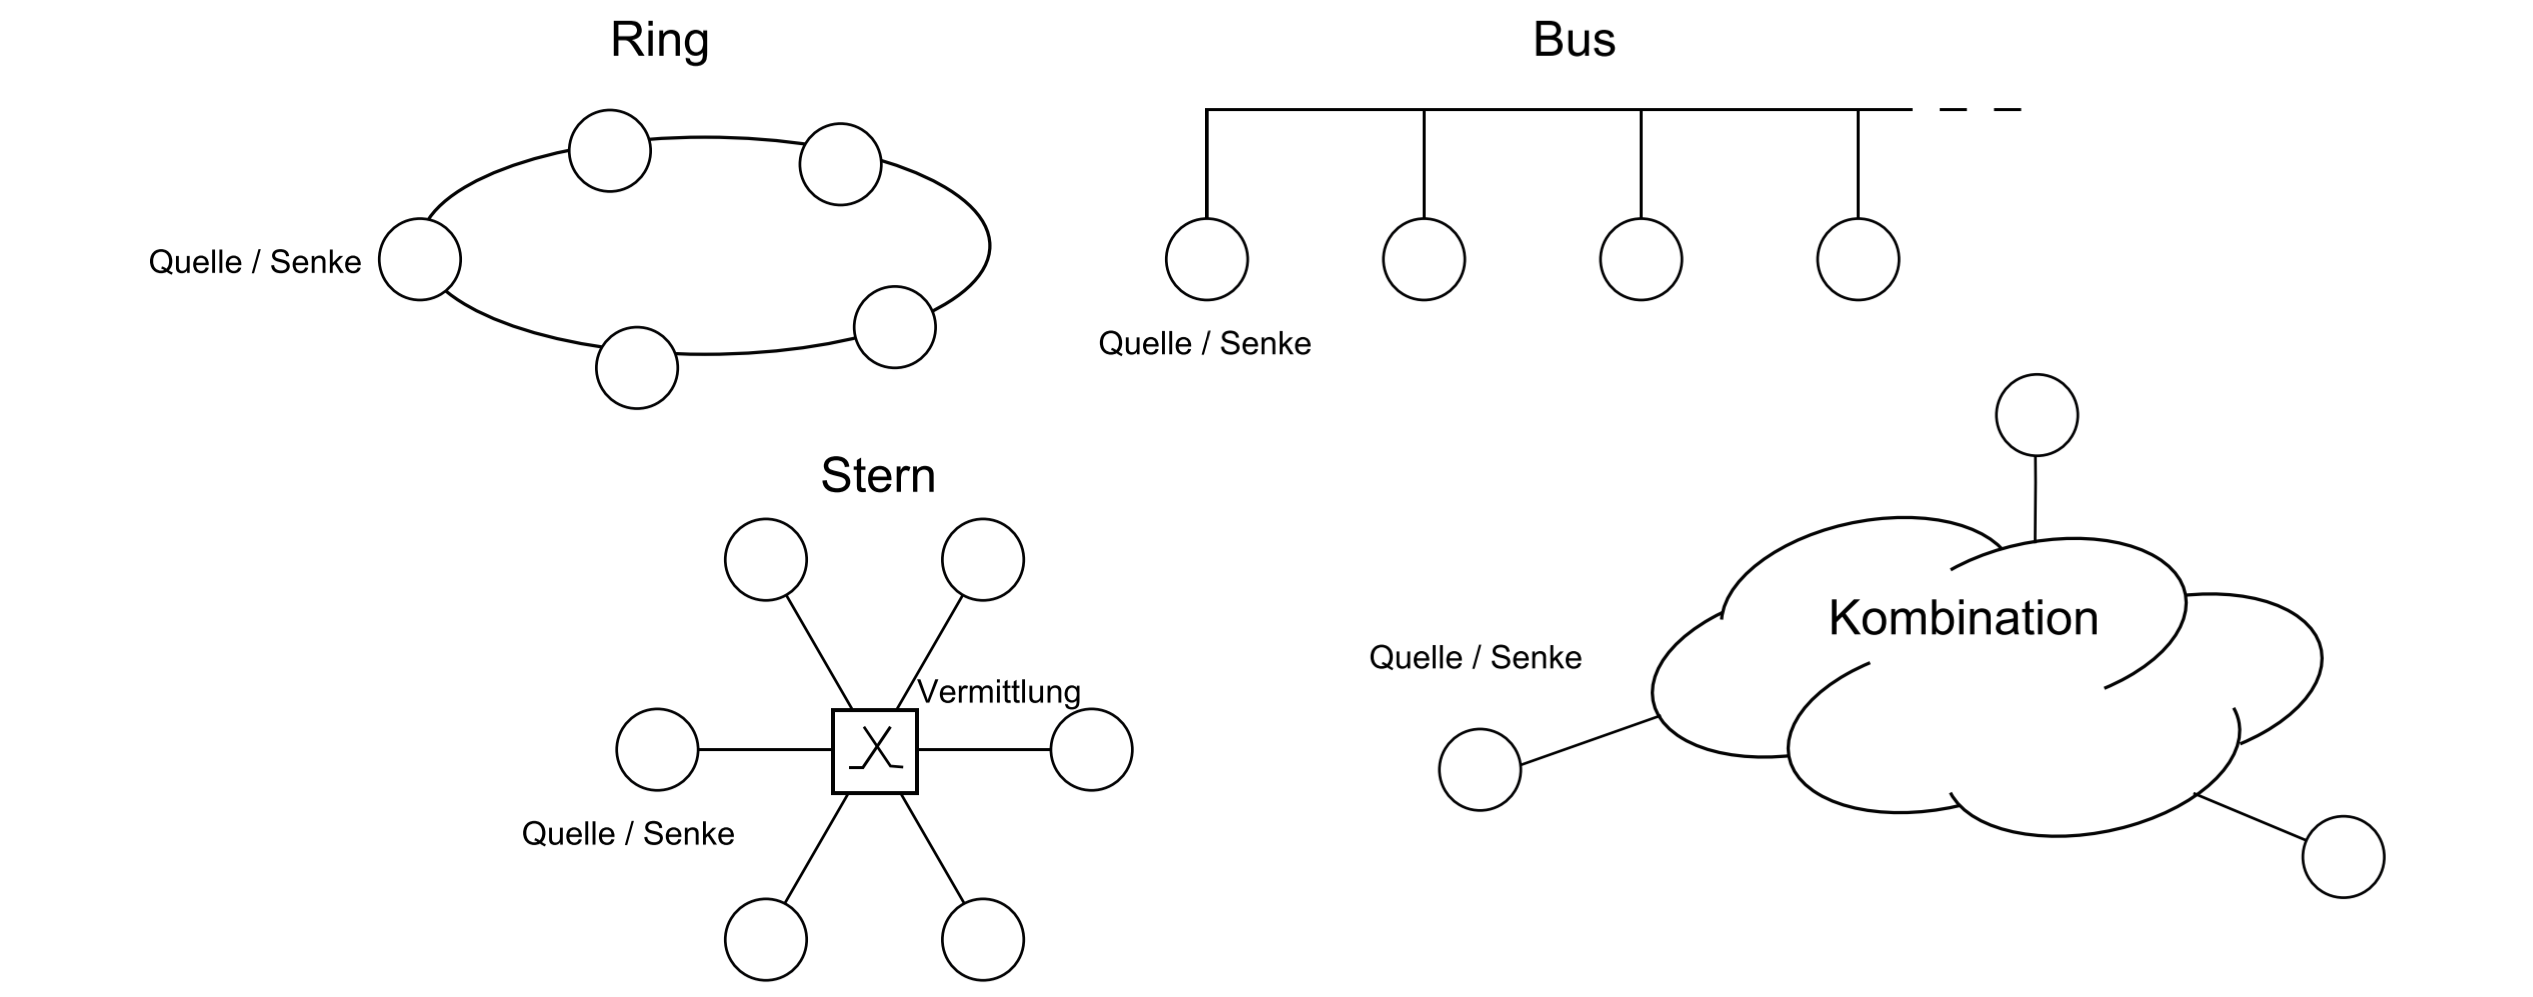
\includegraphics{images/01_Netzstruktur.png}

}

\caption{Gebräuchliche Netzstrukturen}

\end{figure}

\hypertarget{uxfcbertragungskapazituxe4t}{%
\subsubsection{Übertragungskapazität}\label{uxfcbertragungskapazituxe4t}}

Infolge physikalischer Eigenaschaften (endliche Bandbreite,
Rauschen/Störungen) hat jeder Übertragungskanal eine begrenzte Kapazität
für Informationsübertragung. Die \emph{Kapazität} \(C\) hängt von der
verfügbaren \emph{Bandbreite} \(B\) und dem Verhältnis zwischen
\emph{Signalleistung} \(S\) und \emph{Rauschleistung} \(N\)
\emph{(externer Einfluss)} ab.

\[
C = B\cdot log_2\left(1+\frac{S}{N}\right)\qquad [bps]
\]

\begin{figure}[H]

{\centering 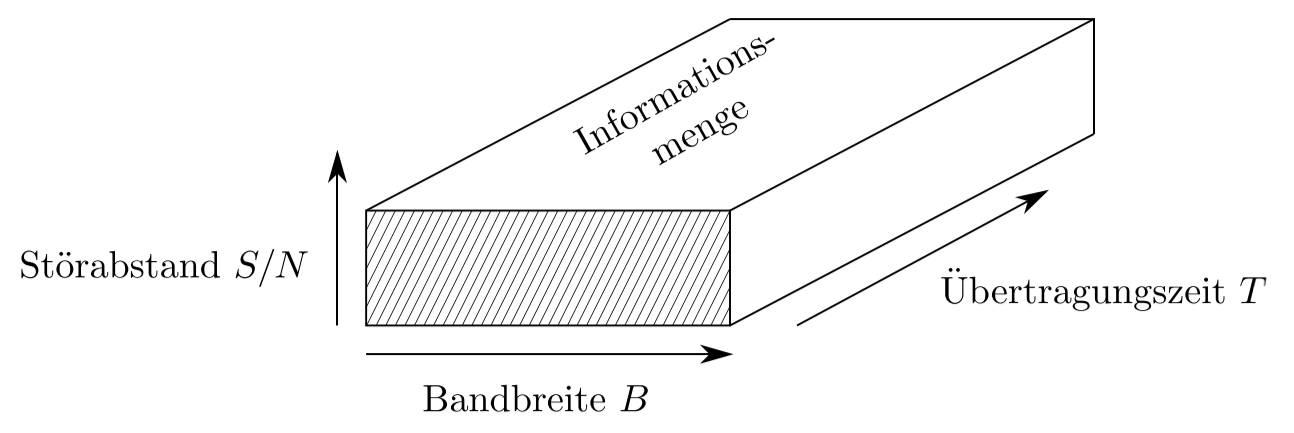
\includegraphics{images/01_Informationsquader.png}

}

\caption{Informationsquader}

\end{figure}

Bei einer Fehlerrate von \(10^{-12}\) ergibt sich \(1\) -*Bitfehler* in
\(10^{12}\) Bits.

Zur mehrfachnutzung eines zur verfügung stehenden Kanals werden
verschiedene Verfahren zur Aufbereitung elektrischer Signale verwendet.

\begin{figure}[H]

{\centering 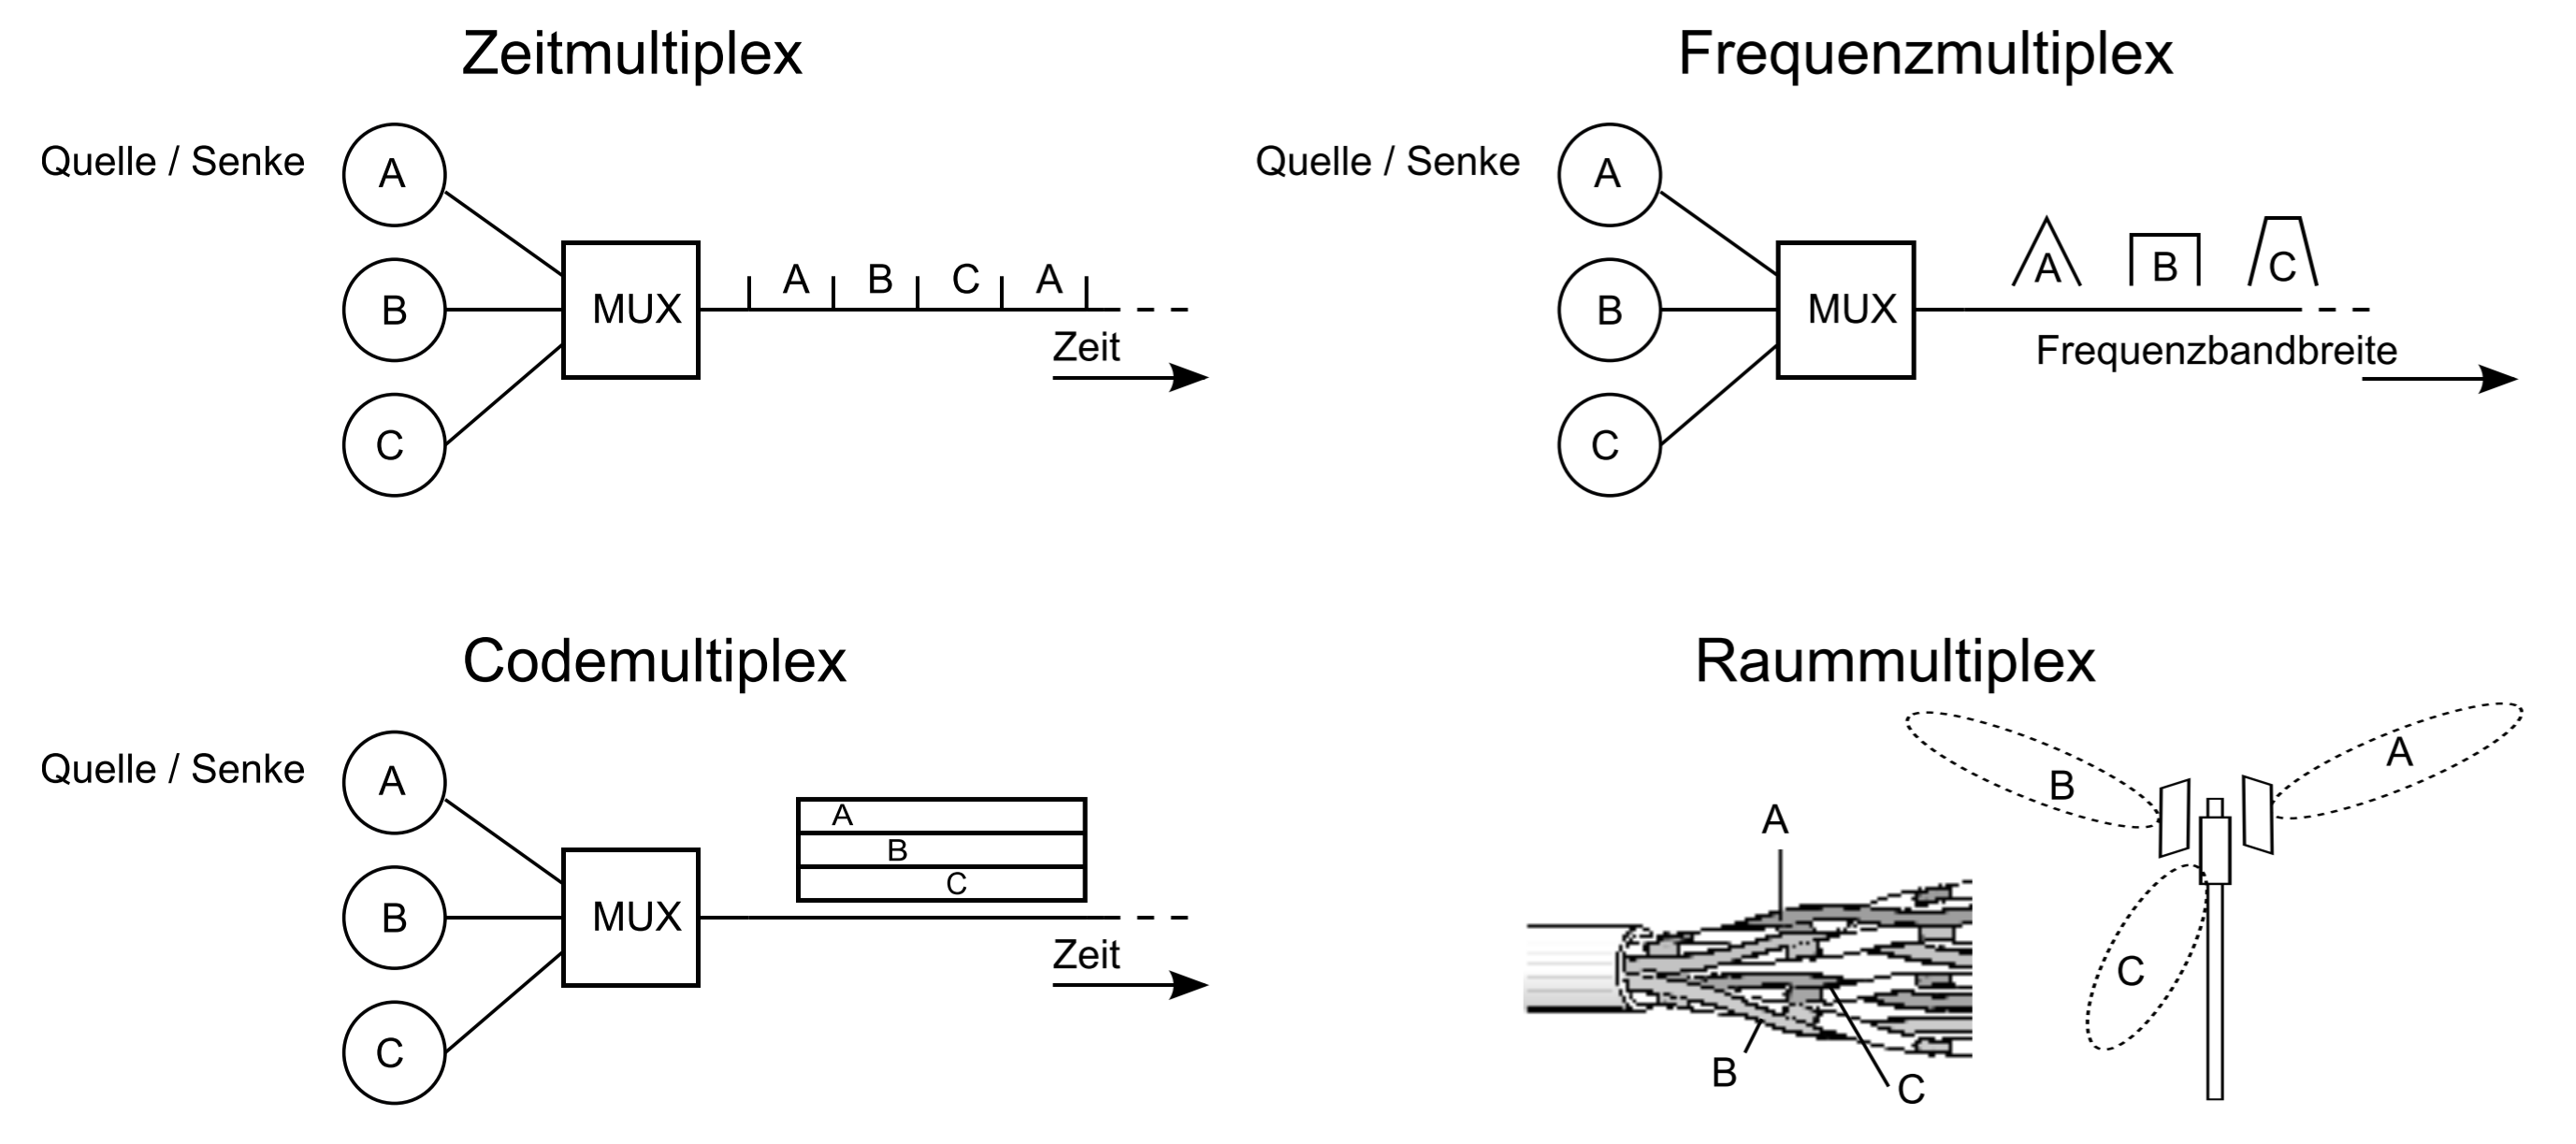
\includegraphics{images/01_Multiplexing.png}

}

\caption{Mehrfachausnutzung mittels Modulation}

\end{figure}

\hypertarget{informationen}{%
\subsection{Informationen}\label{informationen}}

Die Informationsrate einer Quelle ist in der Regel \textbf{nicht
konstant} (Zufallsprozess).

\begin{figure}[H]

{\centering 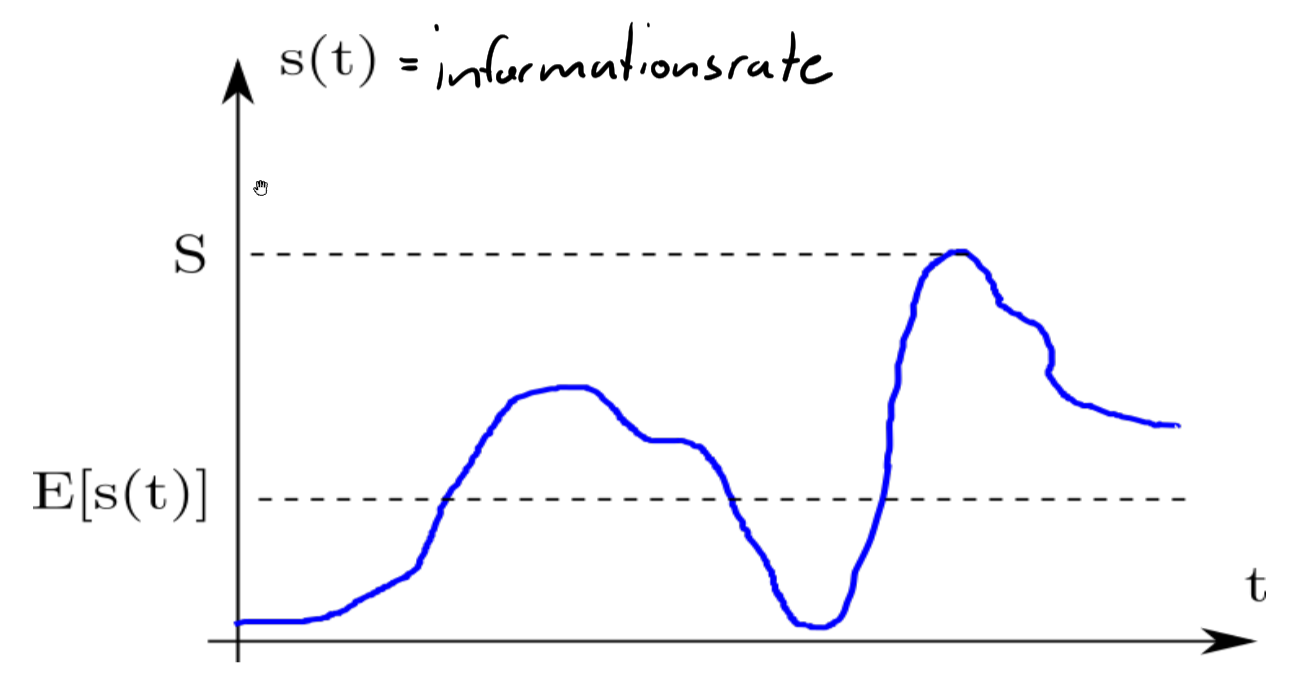
\includegraphics{images/01_Informationsrate.png}

}

\end{figure}

Spitzenwert

\[
S = \max{s(t)}
\]

Erwartungswert

\[
E[s(t)]=\frac{1}{T}\int{s(t)dt}
\]

\hypertarget{qualituxe4t-eines-uxfcbertragungssystems}{%
\subsubsection{Qualität eines
Übertragungssystems}\label{qualituxe4t-eines-uxfcbertragungssystems}}

\hypertarget{stuxf6rfestigkeit-der-uxfcbertragung}{%
\paragraph{Störfestigkeit der
Übertragung}\label{stuxf6rfestigkeit-der-uxfcbertragung}}

Störungen dringen zu einem grossen Teil auf dem Übertragungsweg ein.

\begin{figure}[H]

{\centering 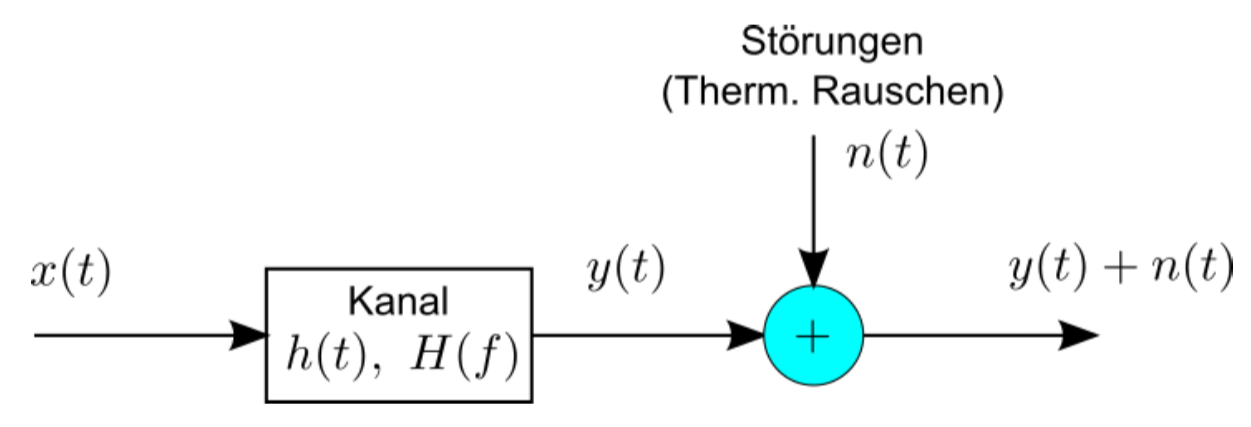
\includegraphics{images/01_Stoerungen.png}

}

\caption{Störquellen}

\end{figure}

Um die Qualität einer Übertragung zu quantifizieren wird der sogenannte
\emph{Störabstand} (\textbf{S}ignal to \textbf{N}oise \textbf{R}ation)
berechnet

\[
SNR=10\cdot\log_{10}\left(\frac{S\space[W]}{N\space[W]}\right)\qquad[dB]
\]

Bei digitaler Übertragung wird die \emph{Bitfehlerrate} (\textbf{B}it
\textbf{E}rror \textbf{R}atio) oder die \emph{Bitfehlerwarscheinlikeit}
\(P_e\) angegeben, welche die Wahrscheinlichkeit angibt, dass ein
Zustand falsch detektiert wird.

\[
P_e=f\left(\frac{S}{N}\right)
\]

\hypertarget{bandbreitenbedarf}{%
\paragraph{Bandbreitenbedarf}\label{bandbreitenbedarf}}

Um möglichst viele \emph{Systeme} \(M\) in einem Kanal mit
\emph{Bandbreite} \(B_K\) unterzubringen, sollte der
\emph{Bandbreitenbedarf} \(B_X\) eines Systems möglichst klein gehalten
werden

\[
M=\frac{B_K}{B_X}
\]

\hypertarget{wiedergabetreue}{%
\paragraph{Wiedergabetreue}\label{wiedergabetreue}}

Die Verzerrung ist bei einem ungestörten Übertragungskanal die Differenz
der Signapegel am Ein- und Ausgang

\[
\varepsilon(t)=y(t)-x(t)
\]

\begin{figure}[H]

{\centering 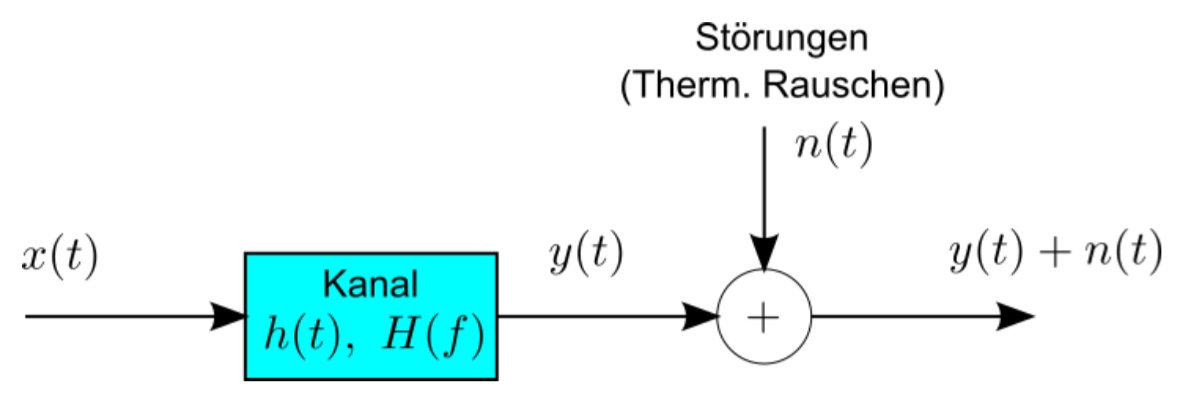
\includegraphics{images/01_Wiedergabetreue.png}

}

\caption{Linearer Übertragungskanal}

\end{figure}

Die Wiedergabe eines Übertragunssystems ist umso besser, je geringer die
Signalverzerrung ist. Eine Verzerrungsfreie Übertragung hat die
Bedingungen \textbf{konstante Verstärkung} und \textbf{linearer
Phasengang}

Eine \emph{Lineare Verzerrung} liegt vor wenn das Ausgangssignal
\textbf{keine zusätzlichen Frequenzkomponenten} enthält.

Um die Wiedergabetreue zu messen wird die \emph{Eintonmessung}
angewendet, bei welcher das Testsignal \(x(t) = \cos(2\pi f_0t)\)
eingespiesen wird und man das Ausgangssignal
\(y(t)=a_1\cos(\omega_0t)+a_2\cos^2(\omega_0t)+...\) erhält. Mit der
Trigonometrischen Umformung

\[
\cos(\alpha)\cos(\beta)=\frac12\cos(\alpha-\beta)+\frac12\cos(\alpha+\beta)
\]

den Therm

\[
y(t)=\underbrace{\left(\frac{a_2}{2}+\frac{3a_4}{8}+...\right)}_{A_0 \space[DC-Anteil]}+
\underbrace{\left(a_1+\frac{3a_3}{4}+...\right)}_{A_1}\cos(\omega_0t)+
\underbrace{\left(\frac{a_2}{2}+\frac{a_4}{4}+...\right)}_{A_2}\cos(2\omega_0t)+...
\]

Zur beschreibung der Nichtlinearität wird der \textbf{Klirrfaktor} \(k\)
benutzt

\[
k=\sqrt{\frac{Oberwellen\space Amplituden}{Gesamt\space Amplituden\space (ohne\space DC)}}=\sqrt{\frac{(A_2)^2+(A_3)^2+...}{(A_1)^2+(A_2)^2+(A_3)^2+...}}
\]

Wird die \emph{Zweitonmessung} \(x(t)=\cos(\omega_1t)+\cos(\omega_2t)\)
gemacht, so enthält das Ausgangssignal eines nichtlinearen Systems neben
den Oberwellen auch die Terme der Form
\((\omega_2-\omega_1),\space(\omega_2+\omega_1),\space(\omega_2-2\omega_1)+...\),
was man als \textbf{Inetrmodulationsprodukte} bezeichnet.

\hypertarget{zeittransparenz-latenz}{%
\paragraph{\texorpdfstring{Zeittransparenz
\emph{Latenz}}{Zeittransparenz Latenz}}\label{zeittransparenz-latenz}}

Die \emph{Latenz} beschreibt in einem Kommunikationsnetz die Einflüsse
einer \emph{Übertragungsverzögerung} und
\emph{Verarbeitungsverzögerung}, wichtige Parameter für Echtzeitdienste.

Die gesamte Verzögerungszeit \(T_{delay}\) besteht aus drei Anteilen

\[
T_{delay}=T_a+T_{\ddot{u}}+T_v
\]

\begin{conditions}
  T_a & Ausbreitungsverzögerung (\textit{propagation delay}) \\
  T_{\ddot{u}} & Übertragungsverzögerung (\textit{transmission delay}) \\
  T_v & Verarbeitungsverzögerung (\textit{process delay}) \\
\end{conditions}

Ausbreitungsverzögerung \emph{propagation delay}

\[
T_a=\frac{\text{Entfernung}\space [m]}{\text{Ausbreitungsgeschwindigkeit}\space[\frac{m}{s}]}\qquad[s]
\]

Übertragungsverzögerung \emph{transmission delay}

\[
T_{\ddot{u}}=\frac{\text{Paketgrösse}\space[byte]}{\text{Datenrate}\space[\frac{bytes}{s}]}\qquad[s]
\]

Die Verarbeitungsverzögerung \emph{process delay} \(T_v\) ist vom
Verarbeitungssystem abhängig und beschreibt z. B. eine Prozesszeit.

\hypertarget{signalanalyse}{%
\section{Signalanalyse}\label{signalanalyse}}

Die Spektralanalyse ist einer der wichtigsten Methoden der Signalanalyse
in der Kommunikationstechnik und basiert auf der Fourier
Reihenentwicklung und der Fourier Transformation. Sie erlaubt im
Frequenzbereich die Behandlung von ganzen Signalklassen mit ähnlichen
Eigenschaften gegenüber der individuellen Analyse jedes einzelnen
Signals im Zeitbereich.

\begin{figure}[H]

{\centering 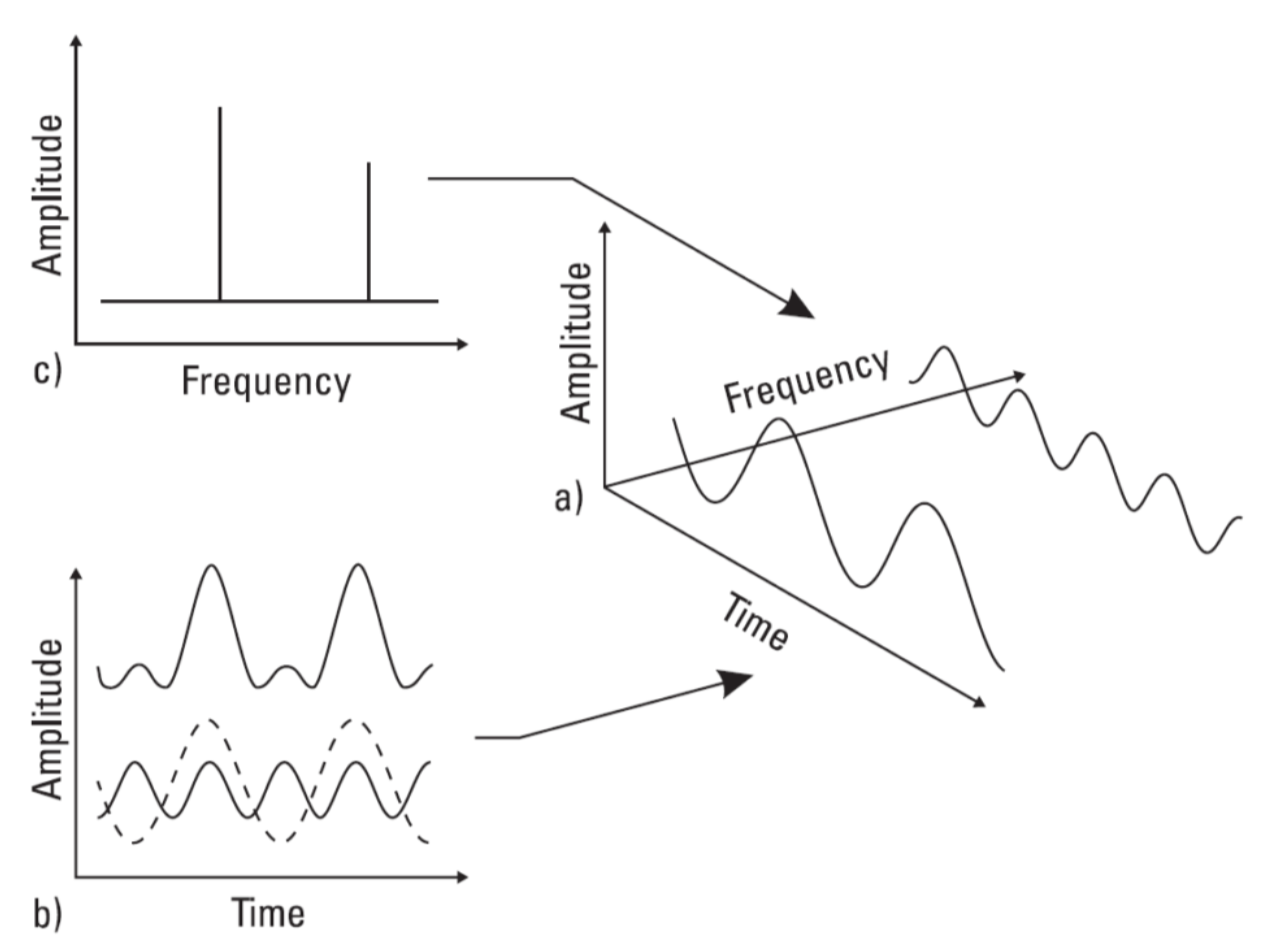
\includegraphics{images/02_Signalanalyse.png}

}

\end{figure}

\hypertarget{deterministische-und-zufallssignale}{%
\subsection{Deterministische und
Zufallssignale}\label{deterministische-und-zufallssignale}}

Signale können entweder \emph{deterministisch} mit mathematischen
Funktionen beschrieben werden oder sie liegen als \emph{Zufallssignale}
vor und nehmen zu jedem Zeitpunkt einen zufälligen Wert an, der einer
Gauss-verteilung folgt.

\hypertarget{harmonische-schwingung}{%
\subsubsection{Harmonische Schwingung}\label{harmonische-schwingung}}

Kosinusschwingung als reelle Zeitfunktion

\[
s(t)=A\cos(2\pi ft+\varphi)
\]

\begin{figure}[H]

{\centering 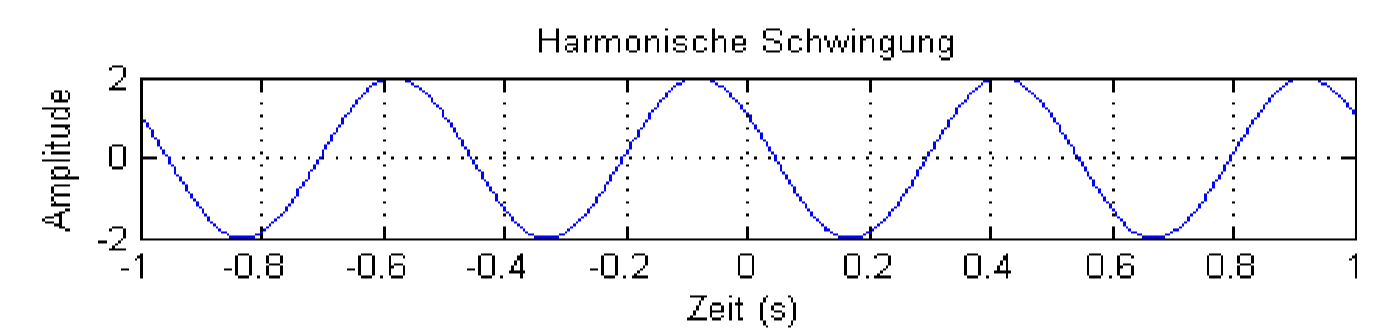
\includegraphics{images/02_HarmonischeSchwingung.png}

}

\end{figure}

\[
+A\sin(\omega t)=+A\cos(\omega t-90°)=+A\cos\left(\omega t -\frac{\pi}{2}\right)
\]

\[
-A\cos(\omega t)=+A\cos(\omega t\pm 180°)=+A\cos(\omega t\pm\pi)
\]

\hypertarget{rechteckpuls}{%
\subsubsection{Rechteckpuls}\label{rechteckpuls}}

\[
\Pi(t)=
\begin{cases}
   1,\qquad|t|<\frac12\\
   0,\qquad\text{sonst}
\end{cases}
\]

\begin{figure}[H]

{\centering 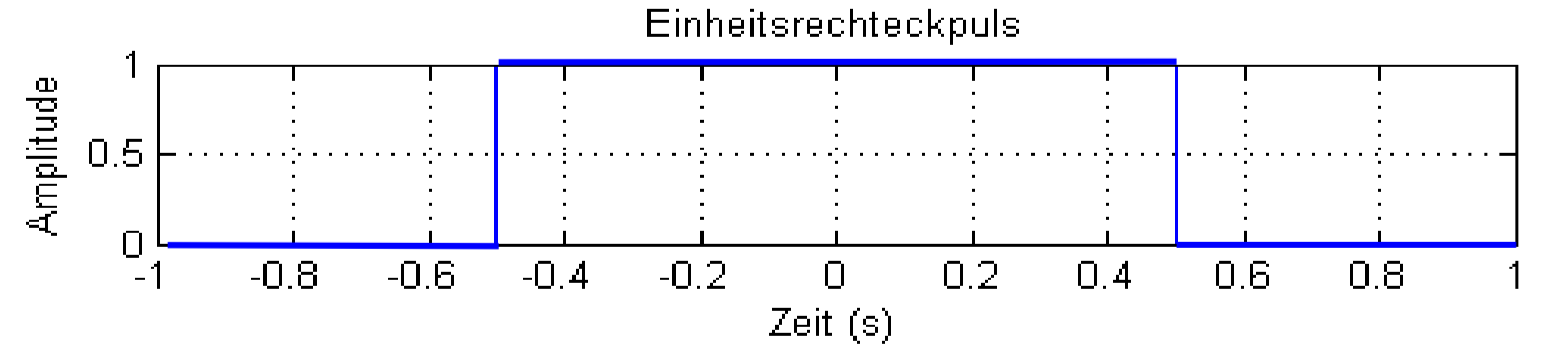
\includegraphics{images/02_Einheitsrechteckimpuls.png}

}

\end{figure}

\hypertarget{zufallssignal}{%
\subsubsection{Zufallssignal}\label{zufallssignal}}

Zufallssignale nehmen zu jedem Zeitpunkt zufällige Werte an und können
daher nicht vollständig mathematisch beschrieben werden. Man kann aber
für diese Signalklasse statistische Grössen wie eine
Wahrscheinlichkeitsdichtefunktion \(p(u)\), den Erwartungswert \(m_u\)
und die Standardabweichung \(s_u\) als beschreibende Grössen ermitteln

\begin{figure}[H]

{\centering 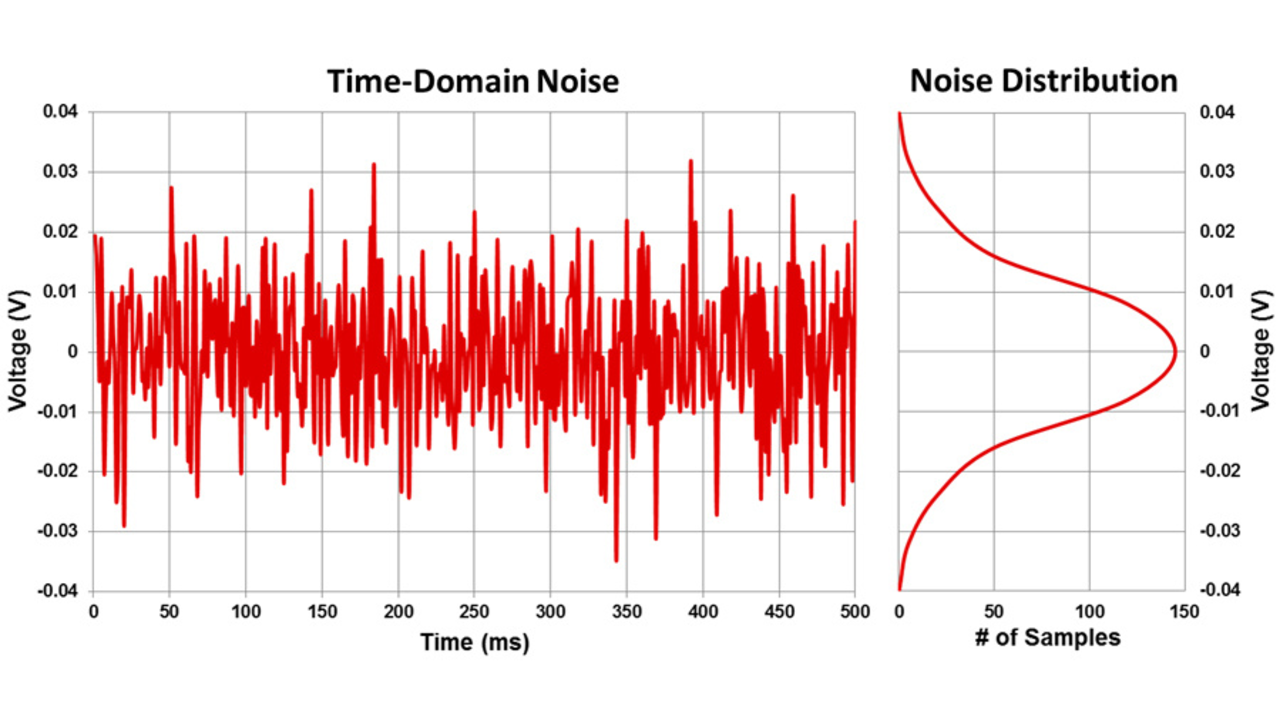
\includegraphics{images/02_Rauschen.png}

}

\end{figure}

\hypertarget{komplexe-zeigernotation}{%
\subsection{Komplexe Zeigernotation}\label{komplexe-zeigernotation}}

Signale (auch Reellwertige) können einfacher anhand der \emph{komplexen
Zeigernotation} beschrieben werden

\[
S(t)=\underbrace{A\cos(\omega_0 t+\varphi)}_{\text{reelle Schwingung}}\pm\underbrace{jA\sin(\omega_0 t+\varphi)}_{\text{Erweiterung}}=\underbrace{Ae^{\pm j(\omega_0 t+\varphi)}}_{\text{komplexer Zeiger}}
\]

Es gilt trotz Erweiterung immernoch

\[
s(t)=Re\left[Ae^{\pm j(\omega_0 t+\varphi)}\right]=A\cos(\omega_0 t+\varphi)
\]

Aus dieser Zeigernotation kann direkt das \textbf{Amplituden- und
Phasenspektrum} als \textbf{einseitiges Linienspektrum} abgetragen
werden

\begin{figure}[H]

{\centering 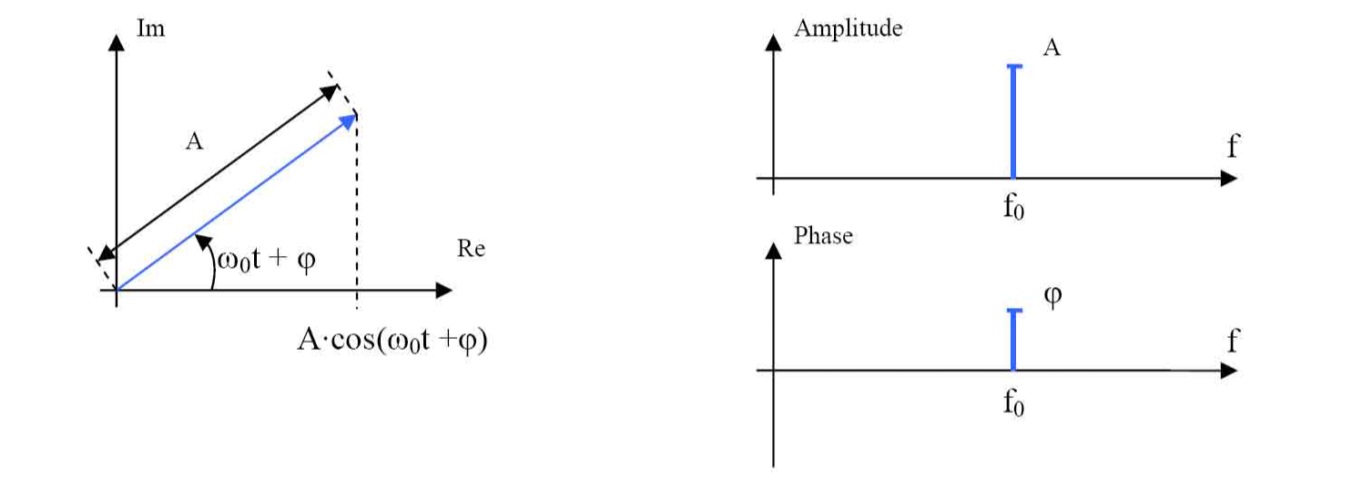
\includegraphics{images/02_AmpUndPhasenSpektrum.png}

}

\caption{Zeigerdiagramm, Amplituden- und Phasenspektrum}

\end{figure}

\hypertarget{zweiseitige-spektrumsdarstellung}{%
\subsubsection{Zweiseitige
Spektrumsdarstellung}\label{zweiseitige-spektrumsdarstellung}}

Eine weitere Darstellung ist das \textbf{zweiseitige Linienspektrum},
wobei über die komplexe Konjugation das Ganze, komplexe Signal
reelwertig gehalten wird

\[
s(t)=\underbrace{\frac{A}{2}e^{j(\omega_0 t+\varphi)}}_{\text{Gegenuhrzeigersinn}}=\underbrace{\frac{A}{2}e^{-j(\omega_0 t+\varphi)}}_{\text{Uhrzeigersinn}}=A\cos(\omega_0 t+\varphi)
\]

da sich die Komplexen Teile aufheben. Da das \emph{Amplitudenspektrum}
stehts den Betrag anzeigt, werden negative Werte stehts mit einer
\emph{Phasenverschiebung} um \(\pi\) aufgetragen.

\begin{itemize}
\item
  Amplitudendiagramm ist \emph{symmetrisch}
\item
  Phasendiagramm ist \emph{punktsymmetrisch}
\end{itemize}

\begin{figure}[H]

{\centering 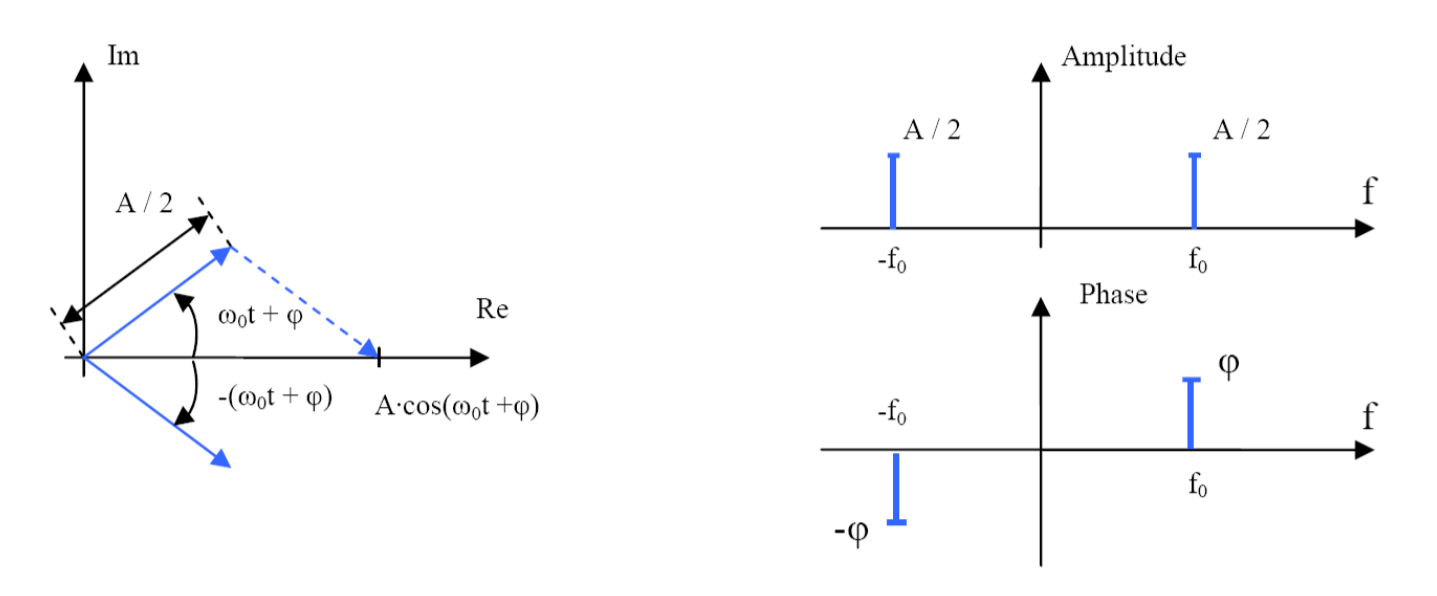
\includegraphics{images/02_AmpUndPhasenSpektrumZweiseitig.png}

}

\caption{Konjugiert komplexe Zeiger und zweiseitiges Linienspektrum}

\end{figure}

\hypertarget{periodische-signale}{%
\subsection{Periodische Signale}\label{periodische-signale}}

Harmonische Schwingungen und Zeiger gehören zu der allgemeinen Klasse
der periodischen Signale, mit der Eigenschaft

\[
s(t\pm mT_0)=s(t)\qquad -\infty<t<+\infty\qquad\text{Mit }m=1,2,3,...
\]

Die Signalform ändert sich also nicht bei einer Verschiebung um \(m\).

\hypertarget{mittlere-leistung}{%
\subsubsection{Mittlere Leistung}\label{mittlere-leistung}}

\emph{Mittelwert} \(\bar{s}\)

\[
\bar{s}=\frac{1}{T_0}\int_{t_0}^{t_0+T_0}{s(t)dt}
\]

Die \emph{Mittlere \textbf{normierte} Leistung} beschreibt die Leistung
bezogen auf \(1\Omega\)

\[
P=\frac{1}{T_0}\int_{t_0}^{t_0+T_0}{|s(t)|^2dt}
\]

Entspricht die Leistung \(0<P<\infty\) so spricht man von einem
\emph{periodischen Leistungssignal}.

\hypertarget{sinc-funktion}{%
\subsection{\texorpdfstring{\(sinc\)-Funktion}{sinc-Funktion}}\label{sinc-funktion}}

Zur Bestimmung der Fourier-Koeffizienten \(c_n\) erhält man oft das
Integral

\[
\frac{1}{T}\int_{-\frac{T}{2}}^{+\frac{T}{2}}{e^{-j\pi ft}dt}
=-\frac{1}{j2\pi fT}(e^{-j\pi fT}-e^{j\pi fT})
\]

was durch die geometrische Beziehung
\((e^{j\theta}-e^{-j\theta})/(j2)=sin(\theta)\) zur \(sinc\)-Funktion
führt

\[
si(\pi fT)=\frac{sin(\pi fT)}{\pi fT}\qquad\overbrace{=}^{x=fT}\qquad sinc(x)=\frac{sin(\pi x)}{\pi x}=
\begin{cases}
   1,\qquad x=0\\
   0,\qquad x=\pm1,\pm2,...
\end{cases}
\]

\begin{figure}[H]

{\centering 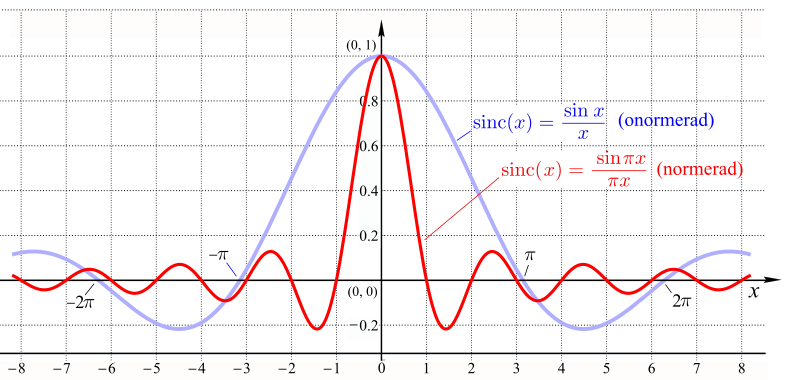
\includegraphics{images/02_sinc.png}

}

\end{figure}

\hypertarget{komplexe-fourier-reihe-perodisch}{%
\subsection{\texorpdfstring{Komplexe Fourier Reihe
\emph{(perodisch)}}{Komplexe Fourier Reihe (perodisch)}}\label{komplexe-fourier-reihe-perodisch}}

Ein periodisches Signal \(s(t)\) kann mit der \emph{komplexen Fourier
Reihenentwicklung} in eine zweiseitige Spektrumsdarstellung gewandelt
werden. DIe komplexe Fourier Riehe für ein periodisches Leistungssignal
der Periode \(T_0=\frac{1}{f_0}\) lautet

\[
s(t)=\sum_{n=-\infty}^{\infty}{c_ne^{jn\omega_0t}}\qquad n=0,\pm1,\pm2,...
\]

Die komplexen Koeffizienten \(c_n\) lauten

\[
c_n=\frac{1}{T_0}\int_{t_0}^{t_0+T_0}{s(t)e^{-jn\omega_0t}dt}
\]

Der Betrag \(|c_n|\) repräsentiert die Amplitude und das Argument
\(\angle c_n\) entspricht der Phase. Es gilt:

\begin{itemize}
\item
  Alle Frequenzen sind ganzzahlige Vielfache der Grundfrequenz
  \(\omega_0\)
\item
  Die Gleichstromkomponente \(c_0\) entspricht \(\bar{s}\)
\item
  Ist \(s(t)\) reell, so besitzt das zweiseitige
  \emph{Amplitudenspektrum} \(|c_n|\) eine \textbf{gerade Symmetrie}
\item
  Ist \(s(t)\) reell, so besitzt das zweiseitige \emph{Phasenspektrum}
  \(\angle c_n\) eine \textbf{ungerade Sysmmetrie}
\end{itemize}

\hypertarget{parsevalsches-leistungstheorem}{%
\subsubsection{Parseval'sches
Leistungstheorem}\label{parsevalsches-leistungstheorem}}

Die mittlere, normierte Leistung eines periodischen Signals kann im
Zeitbereich oder im Frequenzbereich bestimmt werden

\[
P=\frac{1}{T_0}\int_{t_0}^{t_0+T_0}{|s(t)|^2dt}=\sum_{n=-\infty}^{\infty}{|c_n|^2}
\]

\hypertarget{nichtperiodische-energiesignale}{%
\subsection{Nichtperiodische
Energiesignale}\label{nichtperiodische-energiesignale}}

\begin{figure}[H]

{\centering 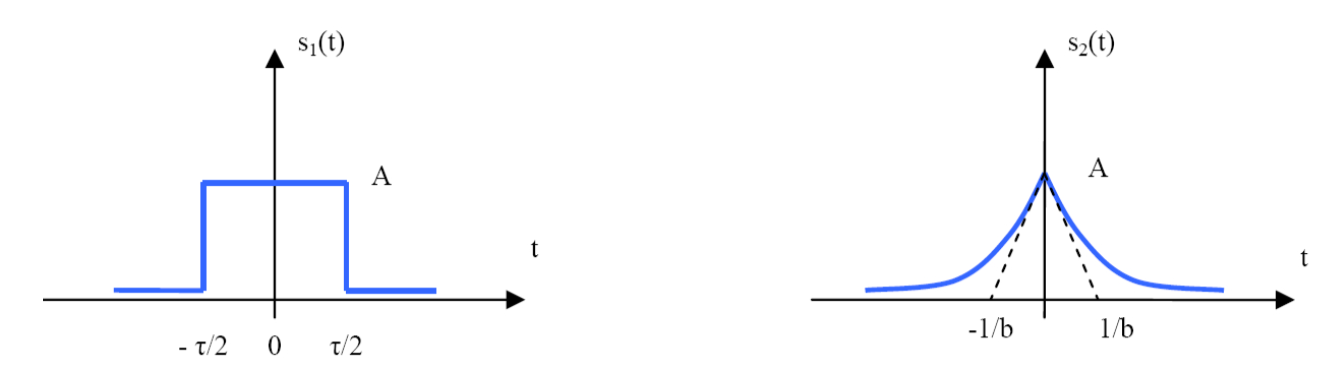
\includegraphics{images/02_NichtPeriodisch.png}

}

\caption{Nichtperiodische Signale}

\end{figure}

Die \emph{normierte Signalenergie} \(E\) beschreibt die Energie eines
Signals über einen Widerstand von \(1\Omega\)

\[
E=\int_{-\infty}^{\infty}{|s(t)|^2dt}
\]

\begin{tcolorbox}[enhanced jigsaw, toptitle=1mm, breakable, colback=white, opacityback=0, colframe=quarto-callout-caution-color-frame, bottomrule=.15mm, toprule=.15mm, bottomtitle=1mm, opacitybacktitle=0.6, coltitle=black, leftrule=.75mm, left=2mm, colbacktitle=quarto-callout-caution-color!10!white, rightrule=.15mm, titlerule=0mm, title=\textcolor{quarto-callout-caution-color}{\faFire}\hspace{0.5em}{Energiesignal}, arc=.35mm]

Ist die Energie \emph{endlich}, also \(0<E<\infty\) so handelt es sich
um ein \textbf{nichtperiodisches Energiesignal}.

Auch Signal die vermeintlich undendlich lange andauern können endlich
sein, z. B.:

\begin{figure}[H]

{\centering 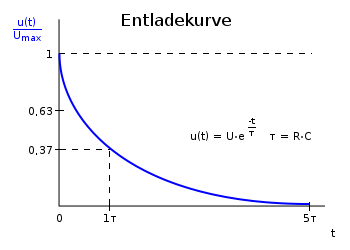
\includegraphics{images/02_Entladekurve.png}

}

\end{figure}

Die Funktion wird zwar Mathematisch nie \(0\), die Energie ist jedoch
Endlich \emph{(Kondensator hat nicht unendlich Energie)}

\end{tcolorbox}

\hypertarget{fourier-transformation-nicht-periodisch}{%
\subsection{\texorpdfstring{Fourier Transformation \emph{(nicht
periodisch)}}{Fourier Transformation (nicht periodisch)}}\label{fourier-transformation-nicht-periodisch}}

Mit der Fourier Transformation werden nicht periodische Signale in ihre
Frequenzbestandteile aufgeteilt und man erhält ein
\textbf{Kontinuierliches Dichtespektrum}. Die Fourier Transformation ist
definiert durch

\[
S(f)=\int_{-\infty}^{\infty}{s(t)e^{-j\omega t}dt}\qquad\text{mit }\omega=2\pi f
\]

Die Rücktransformation gelingt durch die inverse Fourier Transformation

\[
s(t)=\int_{-\infty}^{\infty}{S(f)e^{-j\omega t}dt}\qquad\text{mit }\omega=2\pi f
\]

Für die komplexe Funktion \(S(f)\) der Fourier Transformation gelten die
\emph{spektralen Eigenschaften}

\begin{itemize}
\item
  Das \emph{Amplitudendichtespektrum} entspricht \(|S(f)|\)
\item
  Das \emph{Phasendichtespektrum} entspricht \(\angle S(f)\)
\item
  Der Funktionionswert \(S(f)\big|_{f=0}\) entspricht der Nettofläche
  von \(s(t)\)
\item
  Ist \(s(t)\) reell, so besitzt das \emph{Amplitudenspektrum} \(|c_n|\)
  eine \textbf{gerade Symmetrie}
\item
  Ist \(s(t)\) reell, so besitzt das \emph{Phasenspektrum}
  \(\angle c_n\) eine \textbf{ungerade Sysmmetrie}
\end{itemize}

\hypertarget{parsevalsches-energietheorem}{%
\subsubsection{Parseval'sches
Energietheorem}\label{parsevalsches-energietheorem}}

Die Signalenergie im Zeitbereich wie auch im Grequenzbereich entspricht
demseben Wert, die Beiden Darstellungen beinhalten also diselben
Informationen

\[
E=\int_{-\infty}^{\infty}{|s(t)|^2dt}=\int_{-\infty}^{\infty}{|S(f|^2df}
\]

\hypertarget{logarithmische-darstellung}{%
\subsection{Logarithmische
Darstellung}\label{logarithmische-darstellung}}

Das Amplitudenspektrum wird oft in der y-Achse logarithmisch dargestellt

\[
A_{dB}=20\log_{10}\left(\frac{A_{V}}{A_{Ref}}\right)
\]

als Bezugswert \(A_{Ref}\) wird oft der Effektivwert des Signals oder
die Amplitude der Grundschwingung verwendet.

\hypertarget{korrelation}{%
\subsection{Korrelation}\label{korrelation}}

\hypertarget{autokorrelation}{%
\subsubsection{Autokorrelation}\label{autokorrelation}}

Die \emph{Autokorrelation} macht Angaben über den inneren Zusammenhang
einer Funktion \(s(t)\). Dies gilt für ein \emph{periodisches
Leistungssignal}

\[
k_{11}(t)=E[s_1(t-\tau)\cdot s_1(t)]=\lim_{T\rightarrow \infty}{\frac{1}{T}\int_0^T{s_1(t-\tau)s_1(t)dt}}
\]

und für ein \emph{Energiesignal}

\[
k_{11}(\tau)=\int_{-\infty}^{\infty}{s_1(t-\tau)s_1(t)dt}
\]

Im \textbf{Frequenzbereich} erhalten wir die Autokorrelationen eines
\emph{periodischesn Leistungssignals} durch

\[
k_{11}=\lim_{T\rightarrow\infty}{\frac{1}{T}\int_0^T{S_1(f)S_1^*(f)df}}
\]

und eines \emph{Energiesignals} über

\[
k_{11}(\tau)=\int_{-\infty}^{\infty}{S_1(f)S_1^*(f)df}
\]

\begin{figure}[H]

{\centering 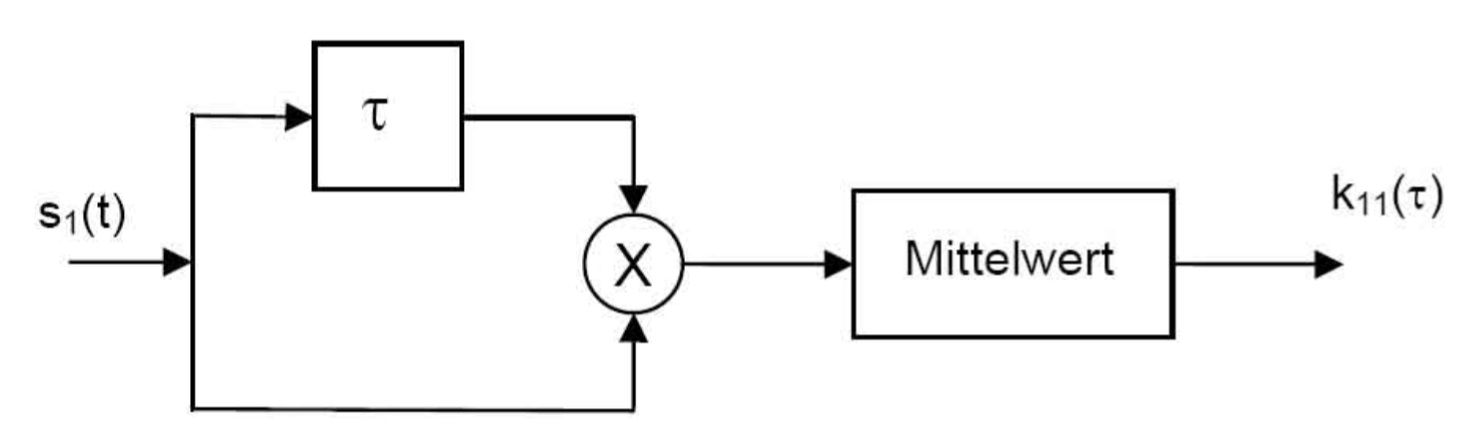
\includegraphics{images/02_Autokorrelation.png}

}

\caption{Blockdiagramm einer Autokorrelation}

\end{figure}

Es gelten die folgenden Eigenschaften:

\begin{itemize}
\item
  \emph{AK} ist gerade: \(k_{11}(\tau)=k_{11}(-\tau)\)
\item
  \(\lim_{\tau\rightarrow\infty}k_{11}(\tau)=0\)
\item
  Bei \(\tau=0\) erhält man die normierte Leistung (o. Energie):
  \(k_{11}(\tau=0)=s_1(t)^2=s_{eff}^2\)
\item
  Das Maximum liegt bei \(\tau=0\)
\item
  Für periodische Signale \(s(t)\) liegt die gleiche Periodendauer wie
  bei \(k_{11}(\tau)\) vor
\end{itemize}

\hypertarget{kohuxe4renzzeit}{%
\paragraph{Kohärenzzeit}\label{kohuxe4renzzeit}}

Der Bereich von \(\tau\), in dem \(k_{11}\ne 0\) ist, wird als
\emph{Kohärenzzeit} bezeichnet.

\begin{figure}[H]

{\centering \includegraphics{images/02_Kohärenzzeit.png}

}

\end{figure}

Die Kohärenzzeit eines sehr fluktiativen (\emph{= grosse Bandbreite})
Signals ist sehr kurz, während diese bei einem langsamen Signal (\emph{=
keline Bandbreite}) eher lang ist. Es gilt also

\[
\text{Kohärenzzeit}\propto \frac{1}{\text{Bandbreite}}
\]

\hypertarget{kreuzkorrelation}{%
\subsubsection{Kreuzkorrelation}\label{kreuzkorrelation}}

Die \emph{Kreuzkorrelation} macht Angaben über den Zusammenhang zweier
Signale \(s_1(t)\) und \(s_2(t)\). Dabei kann man herausfinden, ob zwei
Signale miteinander verwandt sind und gemeinsame Merkmale enthalten.
Zudem kann man erkennen ob zwei Signale in Abhängikeit einer zeitlichen
Verschiebung zueinander stehen. Dies gilt für \emph{periodische
Leistungssignale}

\[
k_{12}(t)=E[s_1(t-\tau)\cdot s_2(t)]=\lim_{T\rightarrow \infty}{\frac{1}{T}\int_0^T{s_1(t-\tau)s_2(t)dt}}
\]

und für ein \emph{Energiesignal}

\[
k_{12}(\tau)=\int_{-\infty}^{\infty}{s_1(t-\tau)s_2(t)dt}
\] Es gelten die folgenden Eigenschaften:

\begin{itemize}
\item
  \emph{KK} ist gerade: \(k_{12}(\tau)=k_{21}(-\tau)\)
\item
  \(\lim_{\tau\rightarrow\infty}k_{12}(\tau)=0\)
\item
  Das Maximum liegt bei \(\tau=\tau_0\)
\end{itemize}

\begin{figure}[H]

{\centering 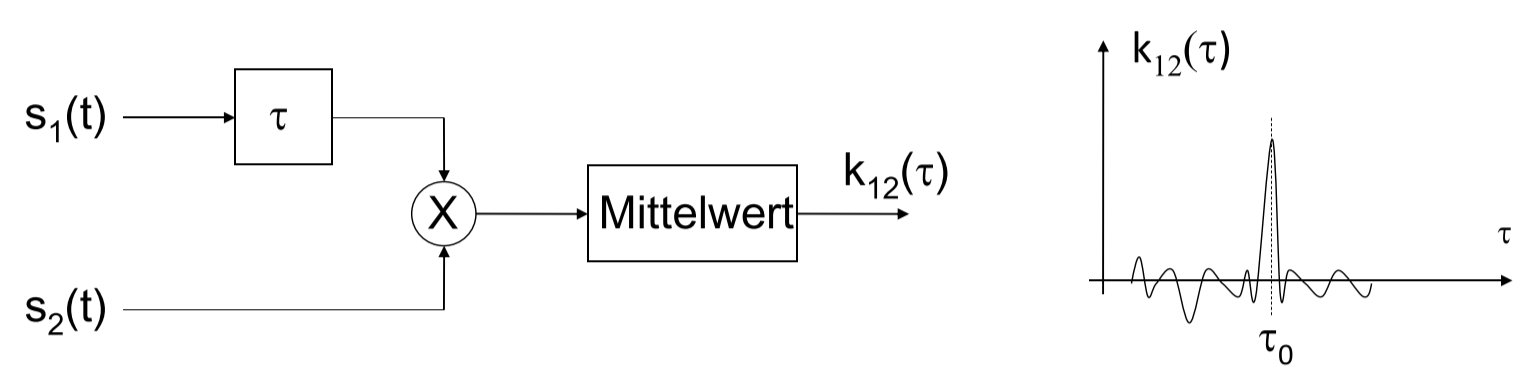
\includegraphics{images/02_Kreuzkorrelation.png}

}

\end{figure}

\hypertarget{signalabtastung-und-rekonstruktion}{%
\subsection{Signalabtastung und
Rekonstruktion}\label{signalabtastung-und-rekonstruktion}}

\hypertarget{idealer-abtastprozess}{%
\subsubsection{Idealer Abtastprozess}\label{idealer-abtastprozess}}

Der Abtastprozess kann als Multiplikation eines analogen Eingangssignals
mit einer periodischen Serie von Einheitsimpulsen betrachtet werden

\[
x(t)=x(t)\sum_{k=-\infty}^{\infty}{\delta(t-kT_s)}
\]

Was eine Faltung im Frequenzbereich mit einem Impulskamm zur Folge hat

\[
X_s(f)=X(f)*\left[f_s\sum_{k=-\infty}^{\infty}{\delta(f-kf_s)}\right]=f_s\sum_{k=-\infty}^{\infty}{X(f-kf_s)}
\]

Was einer periodischen Fortsetzung des Spektrums zur Folge hat

\begin{figure}[H]

{\centering 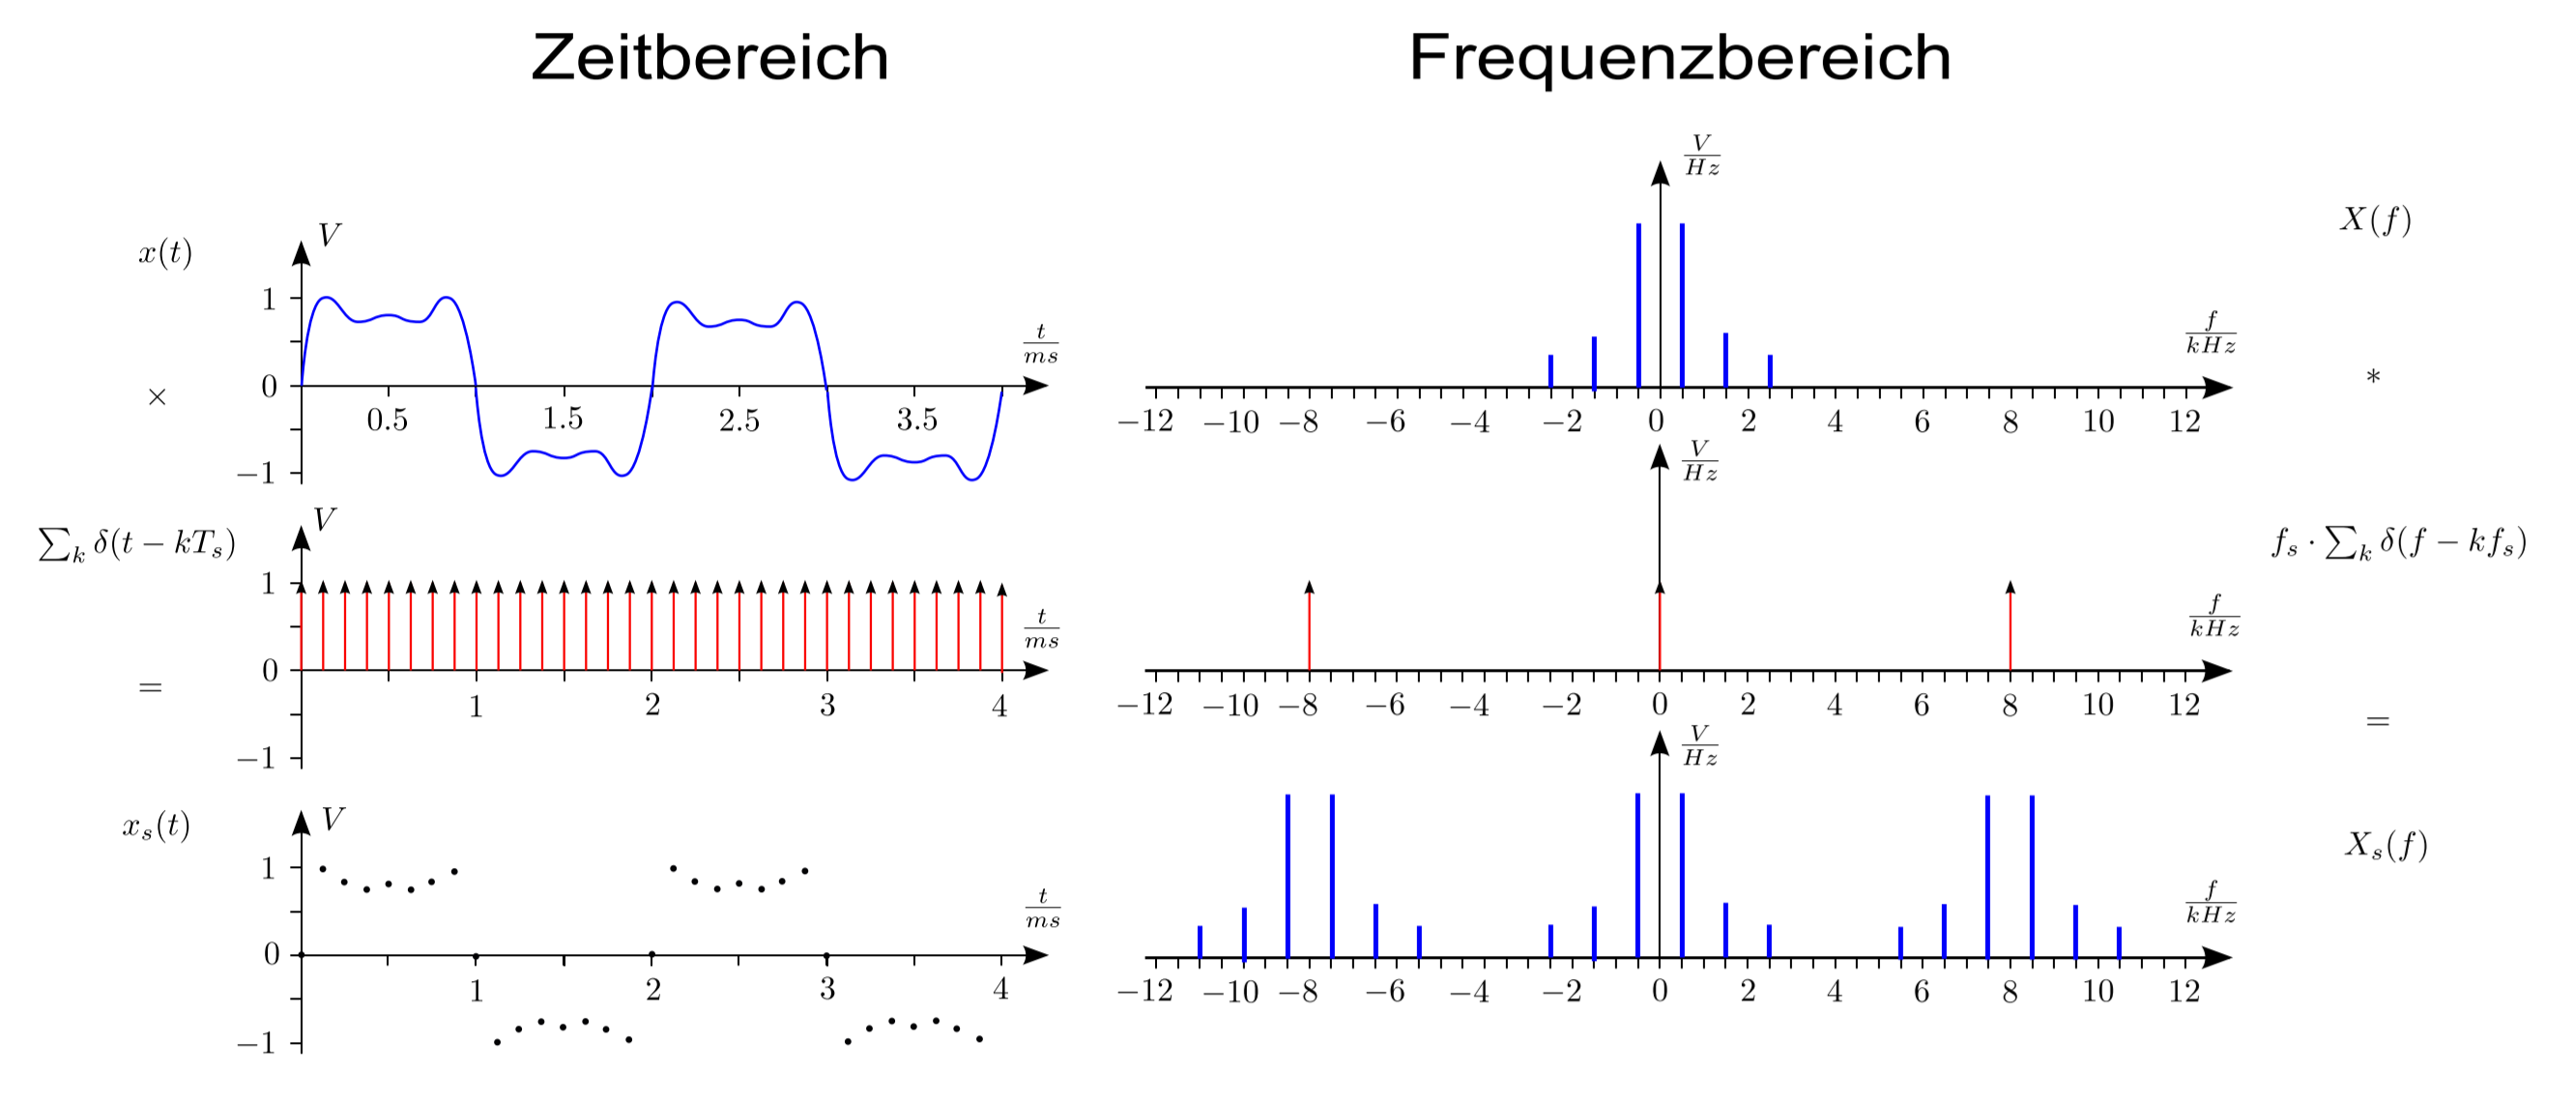
\includegraphics{images/02_IdealeAbtastung.png}

}

\end{figure}

Es sind also Entsprechende Kopien des Spektrums (\emph{Alias}) bei den
ganzzahligen Vielfachen der \emph{Abtastfrequenz} \(f_s\) zu sehen. Die
unverzerrte Rückgewinnung über ein Tiefpassfilter ist nur möglich, wenn
das Abtasttheorem, bzw. die \emph{Nyquist-Rate} eingehalten wird

\[
f_{s_{min}}>2f_{Singal_{max}}
\]

Ein idealer Tiefpass mit einer Verstärkung \(K\), einer Verzögerungszeit
\(t_d\) und einer Bandbreite \(B\) hat eine Übertragungsfunktion von

\[
H_{TP}(f)=K\space \Pi\left(\frac{f}{2B}\right)e^{-j\omega t_d}
\]

\begin{figure}[H]

{\centering 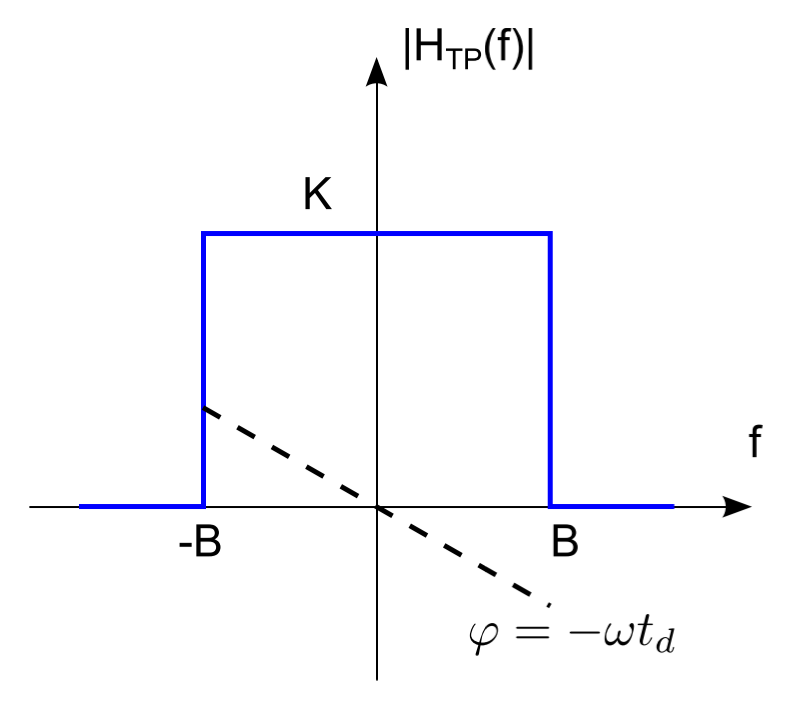
\includegraphics{images/02_IdealerTiefpass.png}

}

\end{figure}

\hypertarget{analoge-vorfilter}{%
\subsubsection{Analoge Vorfilter}\label{analoge-vorfilter}}

Das analoge Vorfilter (\emph{anti-aliasing} Filter) verhindert das
Kopien eines Störignals (Ausserhalb der Grenzfrequenz) in den
Nutzbereich fallen.

\begin{figure}[H]

{\centering 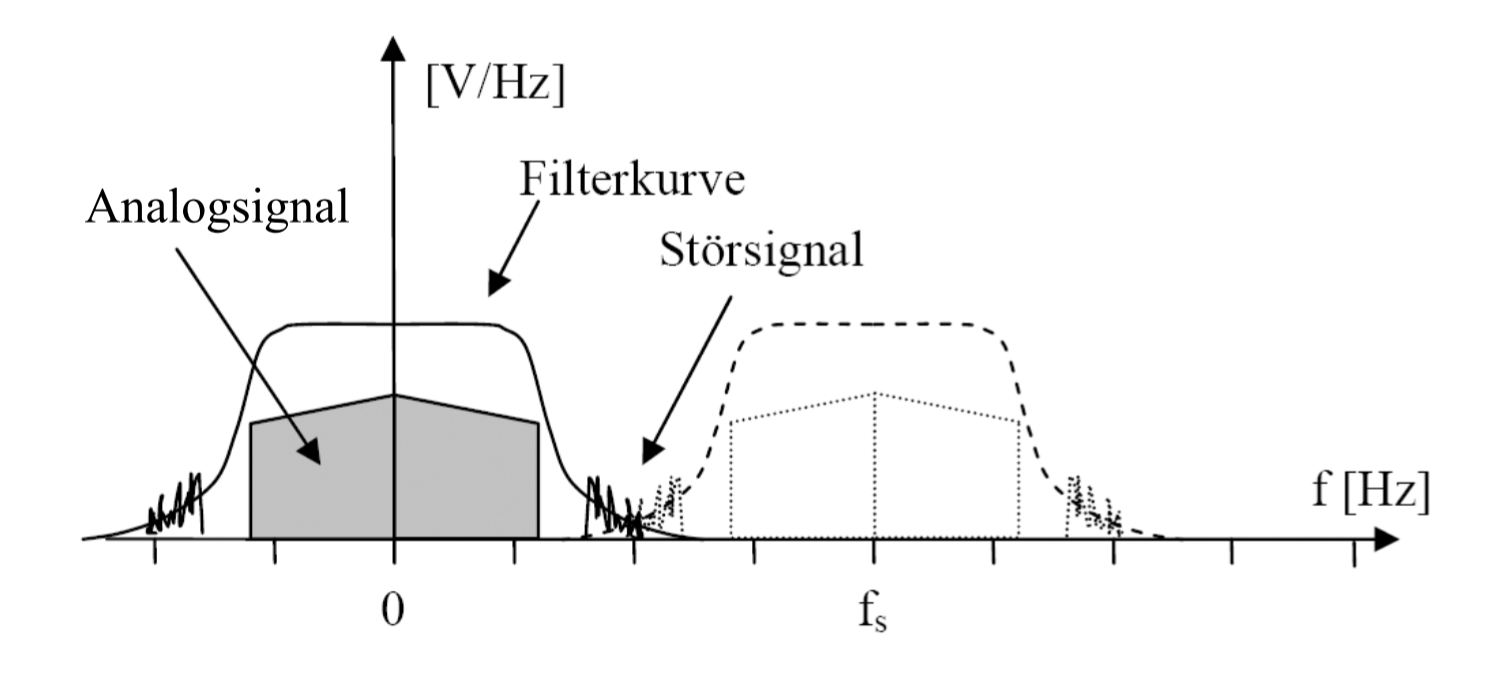
\includegraphics{images/02_AntiAliasing.png}

}

\end{figure}

Realisierbare FIlter sind nicht ideal. Die korrekte Auslegung des
Filters hängt von verschiedenen Gesichtspunkten ab:

\begin{itemize}
\item
  Gewünschte Signalbreite (Grenzfrequenz für den Durchlassbereich
  \(f_g\))
\item
  Abtastfrequenz \(f_s\)
\item
  Gewünschte minimale Sperrdämpfung für Spiegelfrequenzen
  (\(f_{sb}=f_s-f_g\))
\item
  Anforderungen bezüglich Signalverzerrung durch das Filter
\end{itemize}

\hypertarget{reale-abtastung---pam-signal}{%
\subsubsection{Reale Abtastung - PAM
Signal}\label{reale-abtastung---pam-signal}}

Reale Abtastungen erfolgen durch die \emph{Sample\&Hold}-Technik, so
erhält man eine Flat-Top-Abtastung. Dadurch erzeugt man die Zeitfunktion

\[
x_p(t)=x(t)\sum_{k=-\infty}^{\infty}{p(t-kT_s)}
\]

\begin{figure}[H]

{\centering 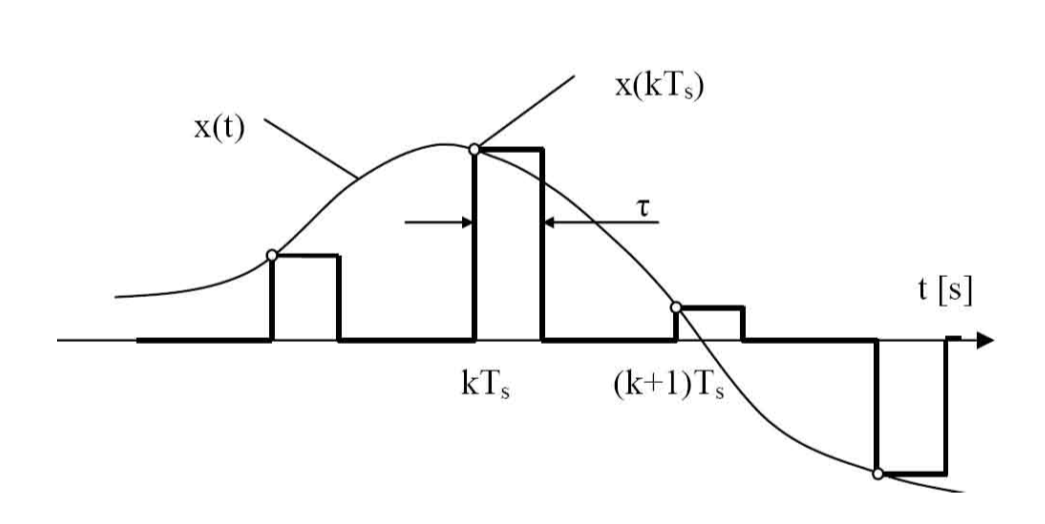
\includegraphics{images/02_FlatTop.png}

}

\end{figure}

Dies induziert einen \emph{Apertureffekt}, bei welchem eine Dämpfung der
höheren Frequenzkomponenten des Signalspektrums

\begin{figure}[H]

{\centering 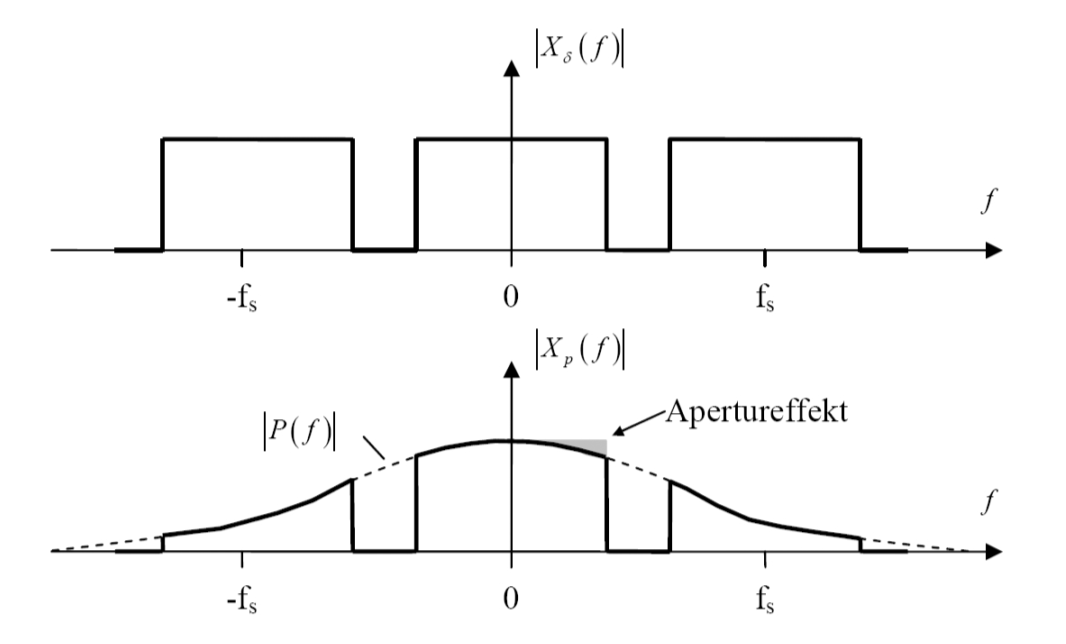
\includegraphics{images/02_ApertureEffekt.png}

}

\end{figure}

\hypertarget{abtastung-von-bandpasssignalen}{%
\subsubsection{Abtastung von
Bandpasssignalen}\label{abtastung-von-bandpasssignalen}}

Besitzt ein Signal ein bandbegrenztes Spektrum mit der Bandbreite \(B\)
und der maximalen oberen Signalfrequenz \(f_{Signal_{max}}\), so kann es
mit der Frequenz

\[
f_{Sample}=\frac{2 f_{Signal_{max}}}{m}
\]

abgetastet werden, ohne das es zu Spektrumsüberlappungen kommt. \(m\)
ist die grösste Zahl, die das Verhältnis \(\frac{f_{Signal_{max}}}{B}\)
nicht übersteigt.

\begin{figure}[H]

{\centering 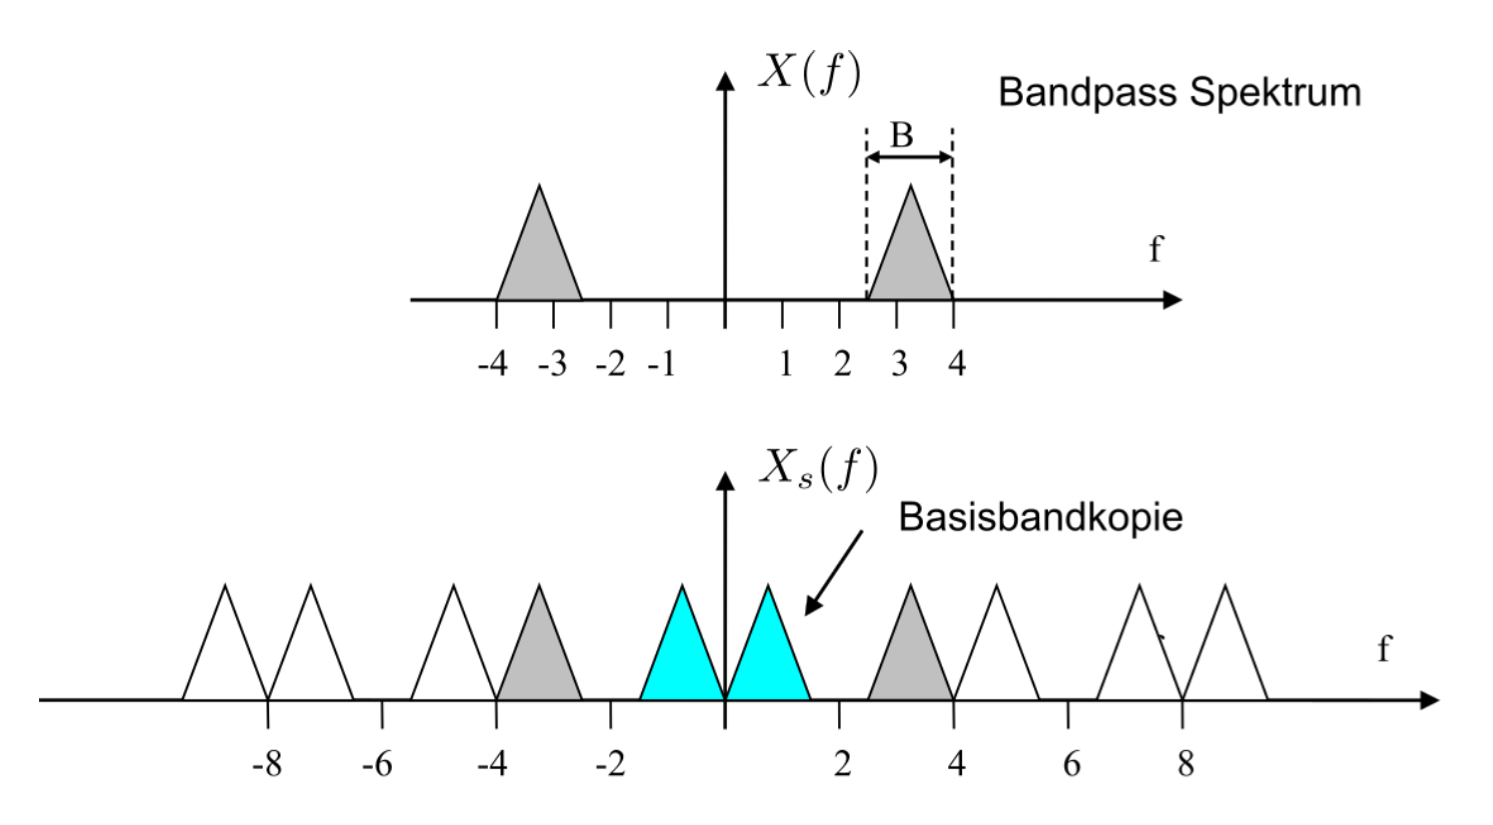
\includegraphics{images/02_BandpassAbtastung.png}

}

\end{figure}

\hypertarget{leitergebundene-signaluxfcbertragung--filterung}{%
\section{Leitergebundene Signalübertragung \&
-Filterung}\label{leitergebundene-signaluxfcbertragung--filterung}}

Es wird hier vorallem vom LTI-Filterkanal gesprochen, und die Störungen
die vom Kanal selbst kommen

\begin{figure}[H]

{\centering 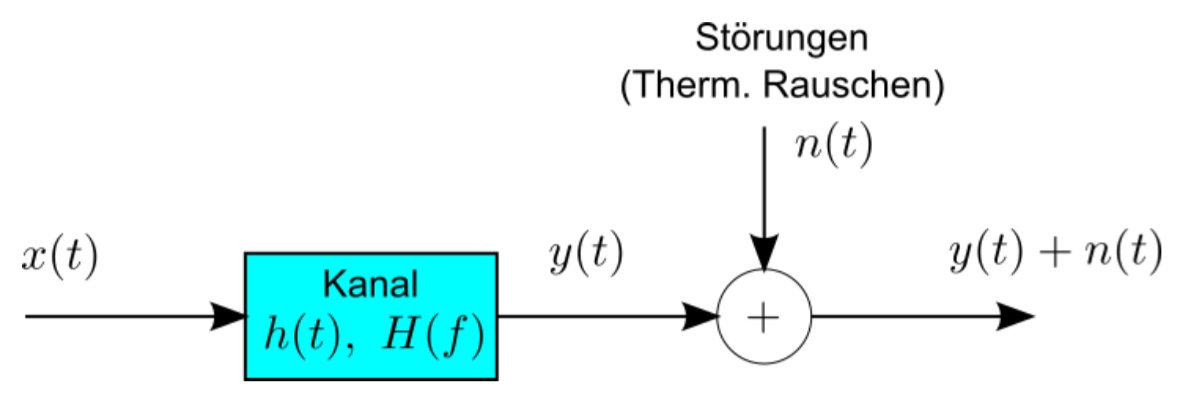
\includegraphics{images/01_Wiedergabetreue.png}

}

\end{figure}

Die Beschreibung der Übertragungseigenschaften erfolgt im Zeitbereich
mithilfe der \emph{Impulsantwort} \(h(t)\) und im Frequenzbereich mit
dem \emph{komplexen Frequenzgang} \(H(f)\). Diese werde folgendermassen
ermittelt

\begin{figure}[H]

{\centering 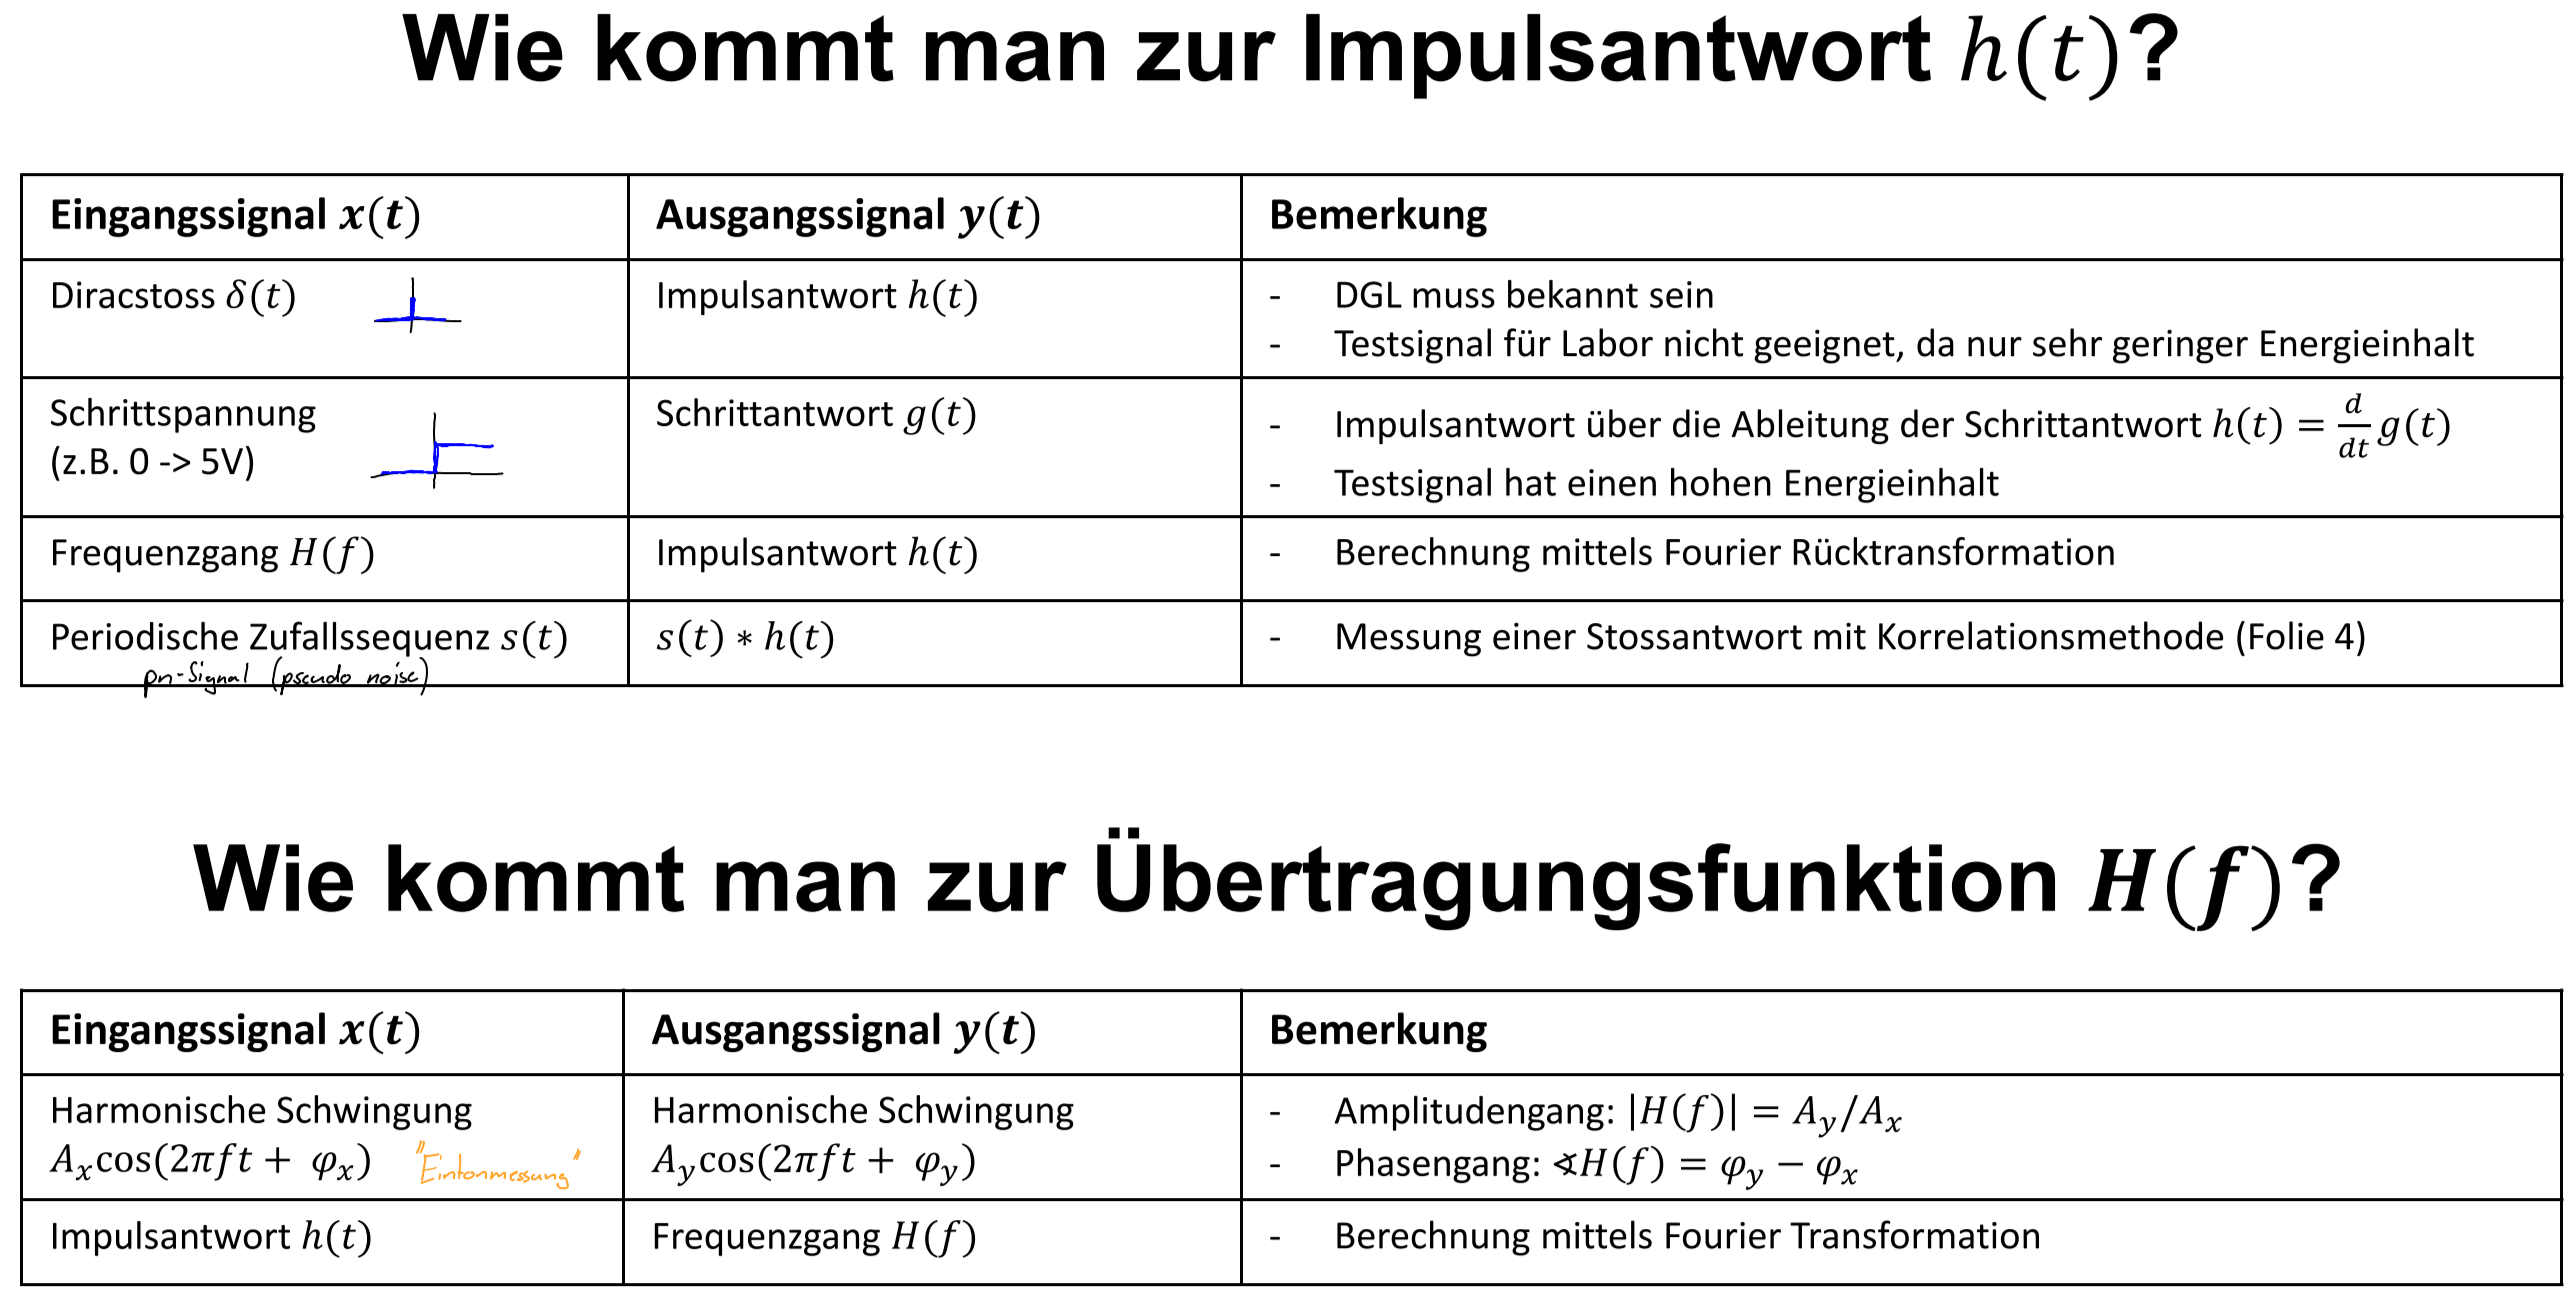
\includegraphics{images/03_uebtertragungsfunktion.png}

}

\end{figure}

Die Ermittlung der Impulsantwort \(h(t)\) mittels \emph{Periodischer
Zufallssequenz} \(s(t)\) erhält man mittels Korrelationsverfahren

\begin{figure}[H]

{\centering 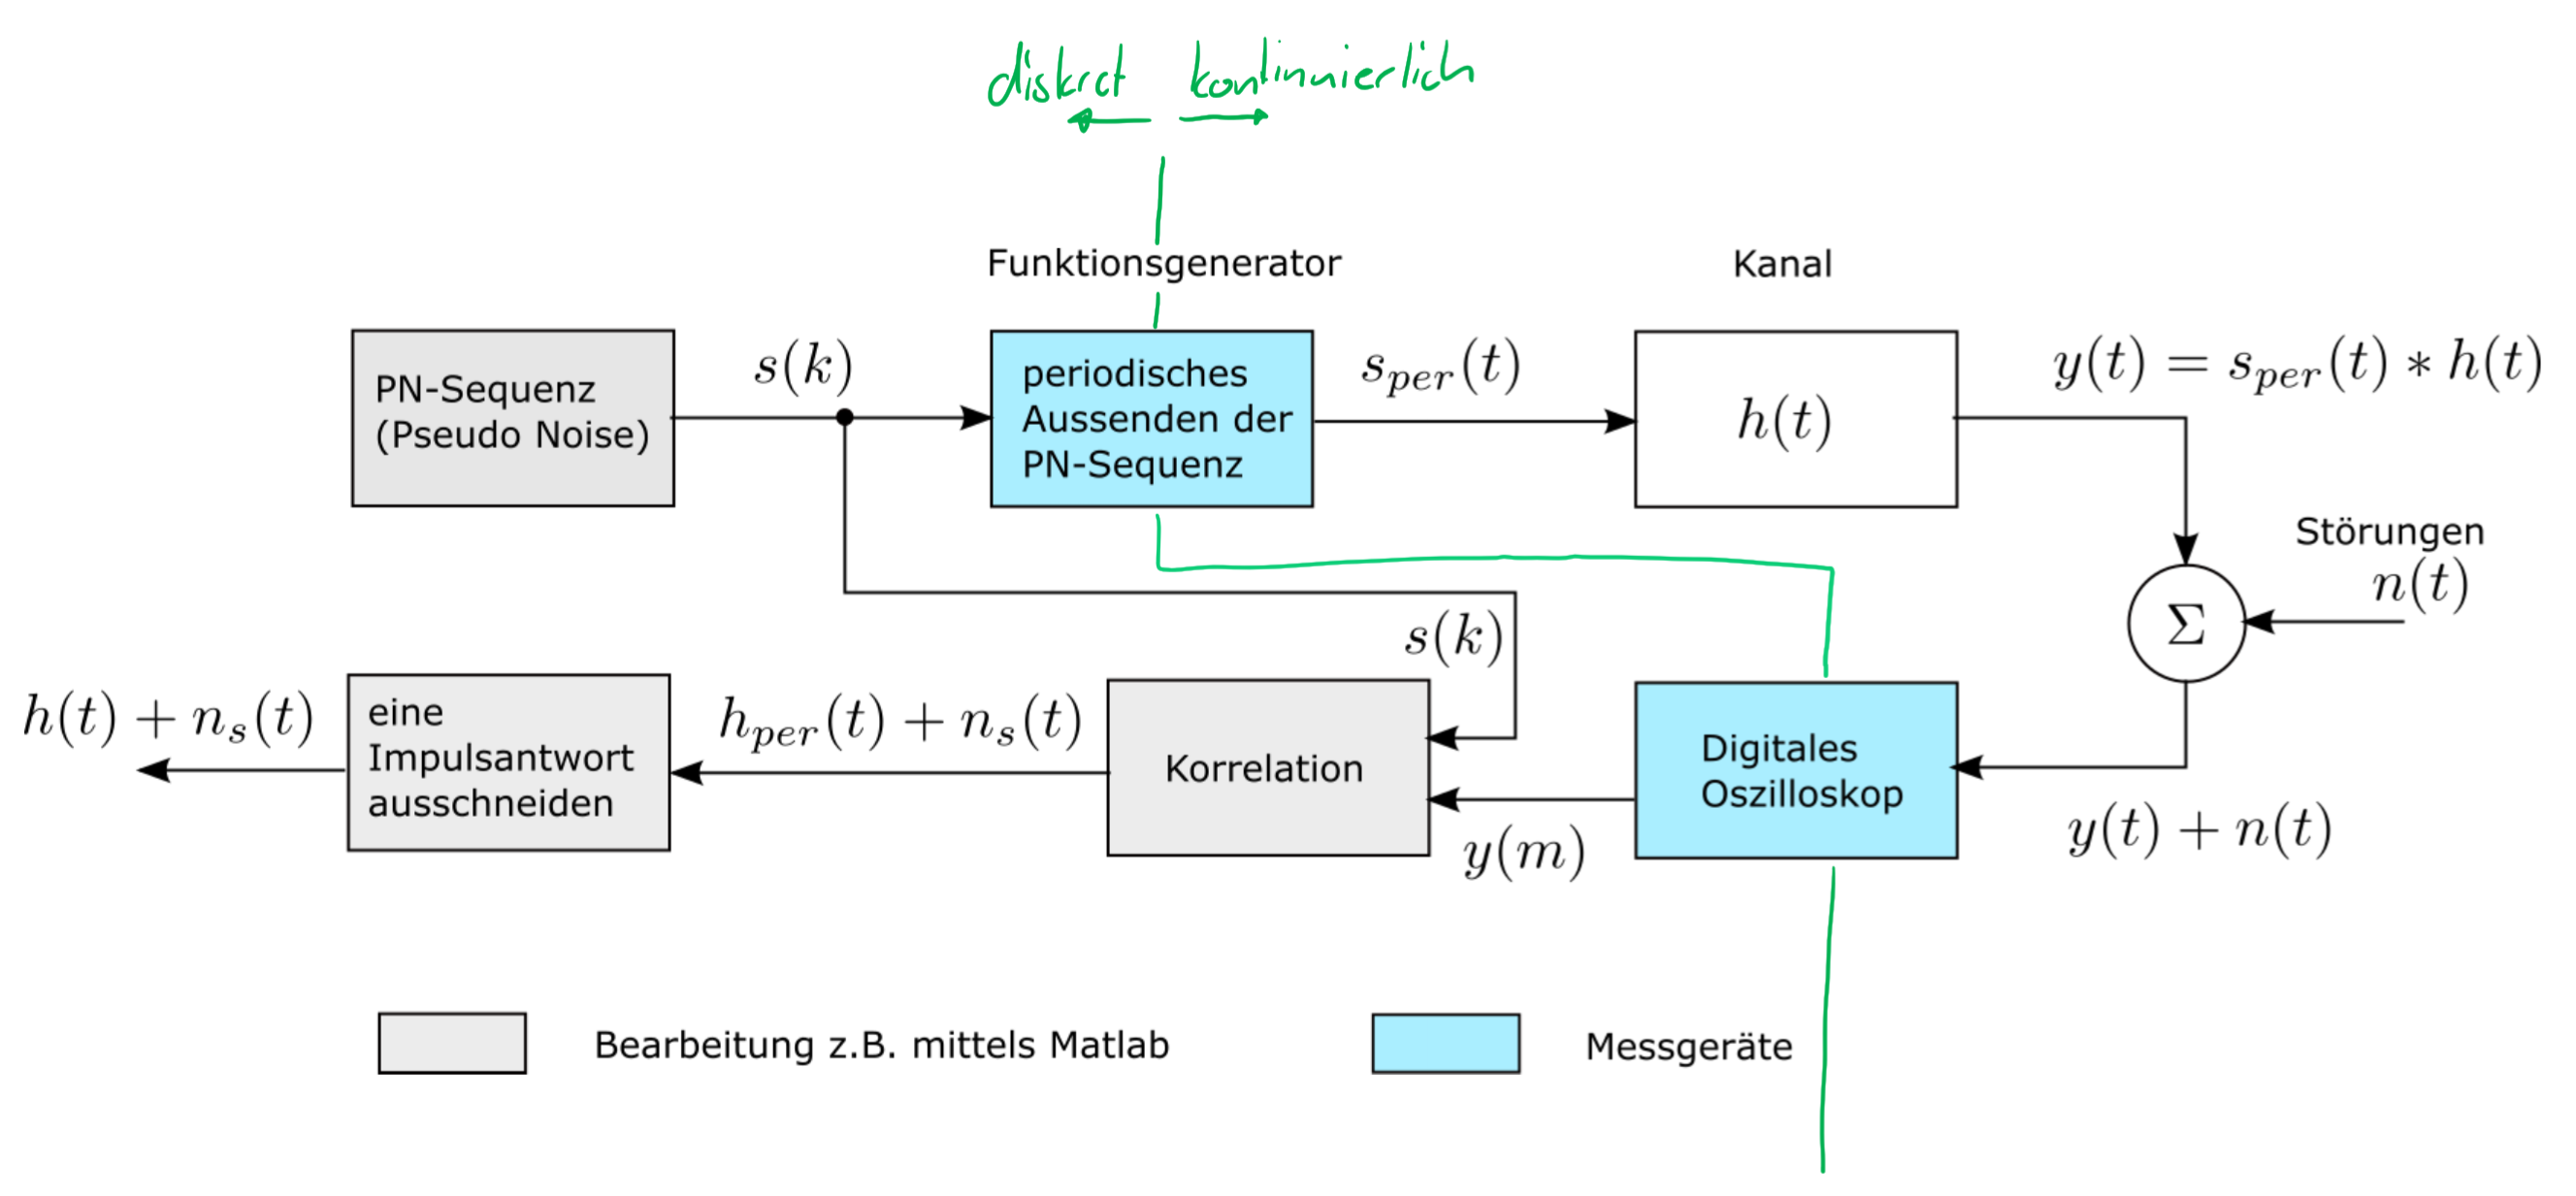
\includegraphics{images/03_Korrelationsverfahren.png}

}

\end{figure}

\hypertarget{pegelberechnung}{%
\subsection{Pegelberechnung}\label{pegelberechnung}}

Bei einer verzerrungsfreien Übertragung ist die Ausgangsleistung \(P_y\)
proportional zur Eingangsleistung \(P_x\) , die \emph{Dämpfung}
entspricht

\[
a=\frac{P_x}{P_y}\qquad\text{bzw.}\qquad a_{dB}=10\space\log_{10}(a)
\]

Können nicht beide Leistungen gleichzeitig bestimmt werden, so wird mit
Referenzgrössen gearbeitet

\begin{longtable}[]{@{}
  >{\raggedright\arraybackslash}p{(\columnwidth - 4\tabcolsep) * \real{0.2639}}
  >{\raggedright\arraybackslash}p{(\columnwidth - 4\tabcolsep) * \real{0.4722}}
  >{\raggedright\arraybackslash}p{(\columnwidth - 4\tabcolsep) * \real{0.2639}}@{}}
\toprule\noalign{}
\begin{minipage}[b]{\linewidth}\raggedright
Referenz
\end{minipage} & \begin{minipage}[b]{\linewidth}\raggedright
Formel
\end{minipage} & \begin{minipage}[b]{\linewidth}\raggedright
Einheit
\end{minipage} \\
\midrule\noalign{}
\endhead
\bottomrule\noalign{}
\endlastfoot
\(P_{Ref}=1mW\) & \(P_{dB}=10\space\log_{10}\left(\frac{P}{1mW}\right)\)
& \(dBm\) \\
\(P_{Ref}=1W\) & \(P_{dB}=10\space\log_{10}\left(\frac{P}{1W}\right)\) &
\(dBW\) \\
\(U_{Ref}=1V\) &
\(U_{dB}=20\space\log_{10}\left(\frac{P}{1V}\right)+10\space\log_{10}\left(\frac{R_{Ref}}{R}\right)\)
& \(dBV\) \\
\(E_{Ref}=1\frac{\mu V}{m}\) &
\(E_{dB}=20\space\log_{10}\left(\frac{P}{1\frac{\mu V}{m}}\right)\) &
\(dB\frac{\mu V}{m}\) \\
\end{longtable}

\hypertarget{filtersysteme}{%
\subsection{Filtersysteme}\label{filtersysteme}}

Niederfrequent haben Analoge LC-FIlter sehr lange eine dominierende
Rolle, wobei dieselben Methoden der Filtersynthese auch auf modernere
Filtertechnologien angewendet werden können. Für verschiedene
Einsatzbereiche gibt es \emph{verschiedene Filtertechnologien}, wobei
auch \emph{Digitale Filter} bis ca. 100MHz analoge Filter nachbilden
können, mit dem VOrteil, dass diese anschliessend noch anpassbar sind

\begin{figure}[H]

{\centering 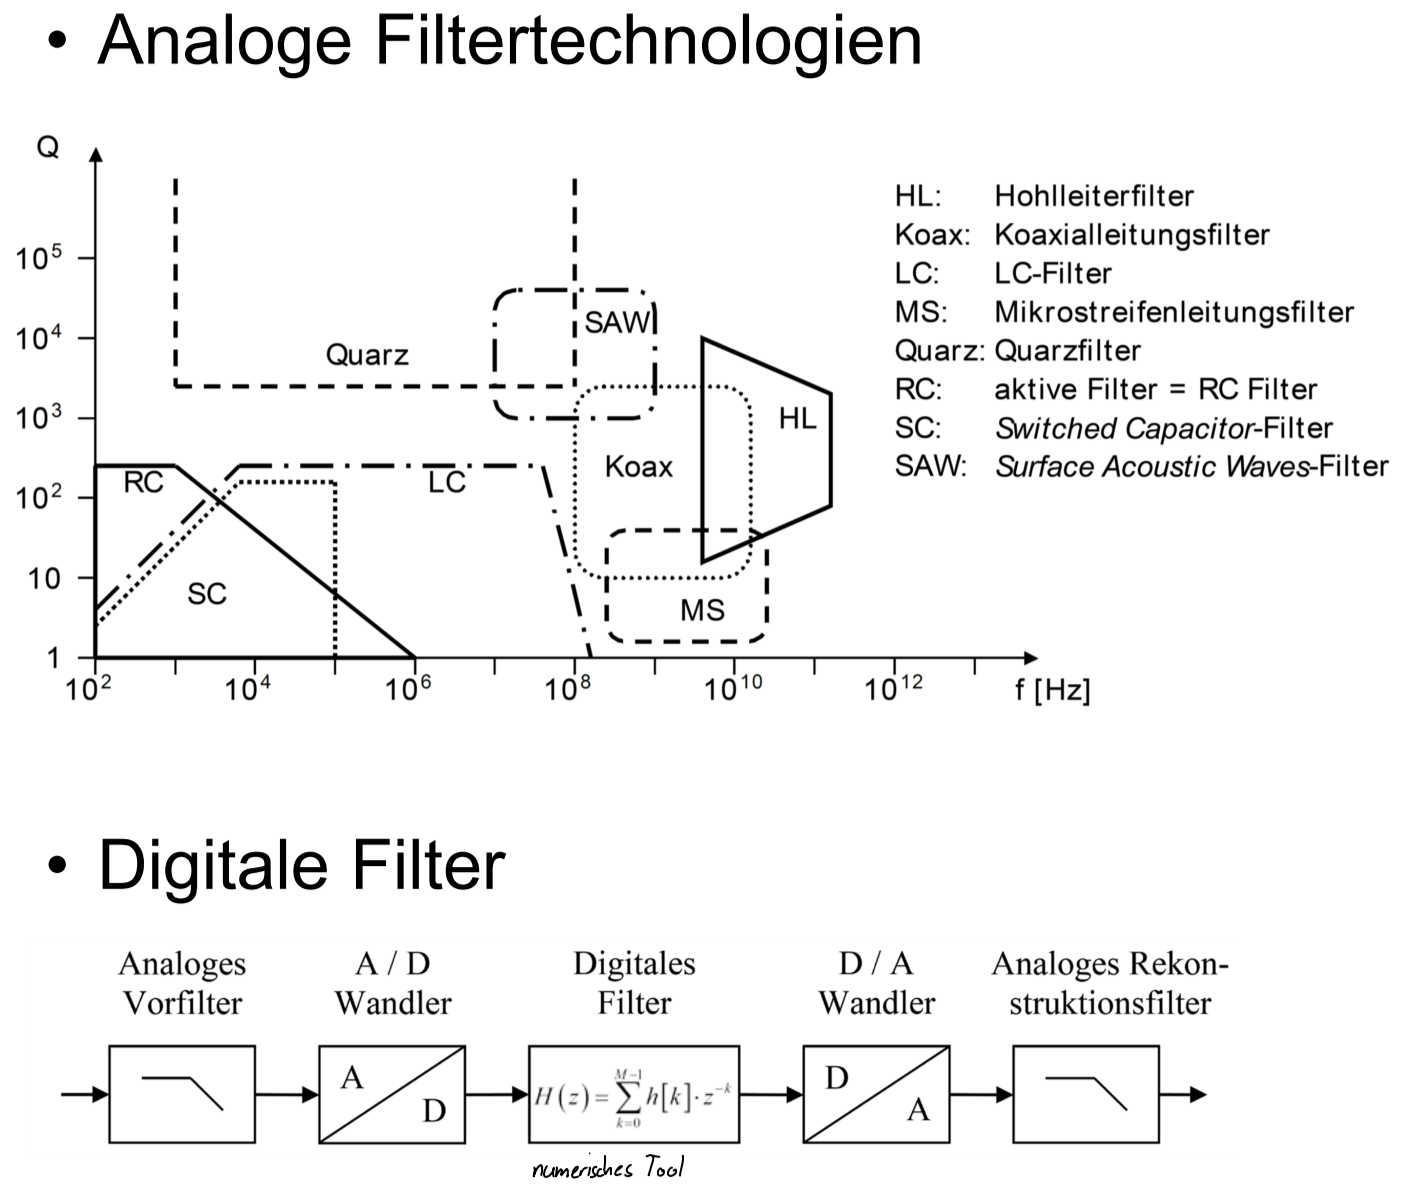
\includegraphics{images/03_Filtertechnologien.png}

}

\end{figure}

Desweiteren gibt es verschiedene Filterklasifizierungen, welche folgende
\textbf{ideale Amplitudengänge} aufweisen

\begin{figure}[H]

{\centering 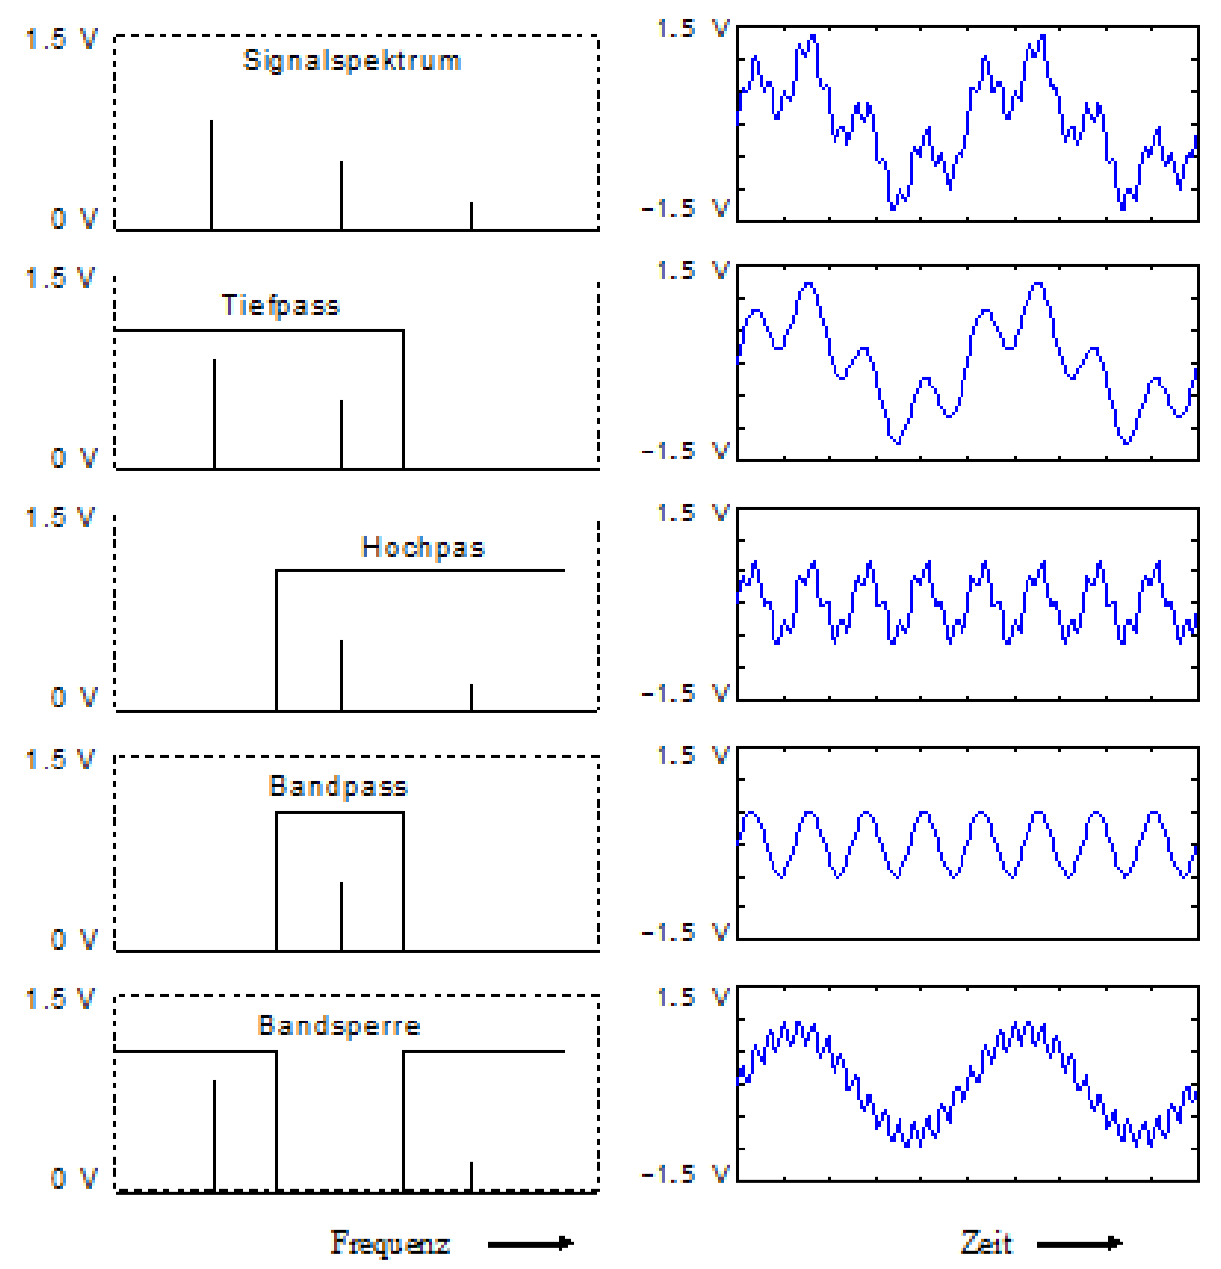
\includegraphics{images/03_Filterklasifizierungen.png}

}

\end{figure}

\hypertarget{reale-filter---spezifikation}{%
\subsubsection{Reale Filter -
Spezifikation}\label{reale-filter---spezifikation}}

Reale Filter können keine sauberen 1/0-Übergänge realisieren, wonach
Filter mit der \emph{Filtermaske} definiert werden

\begin{figure}[H]

{\centering 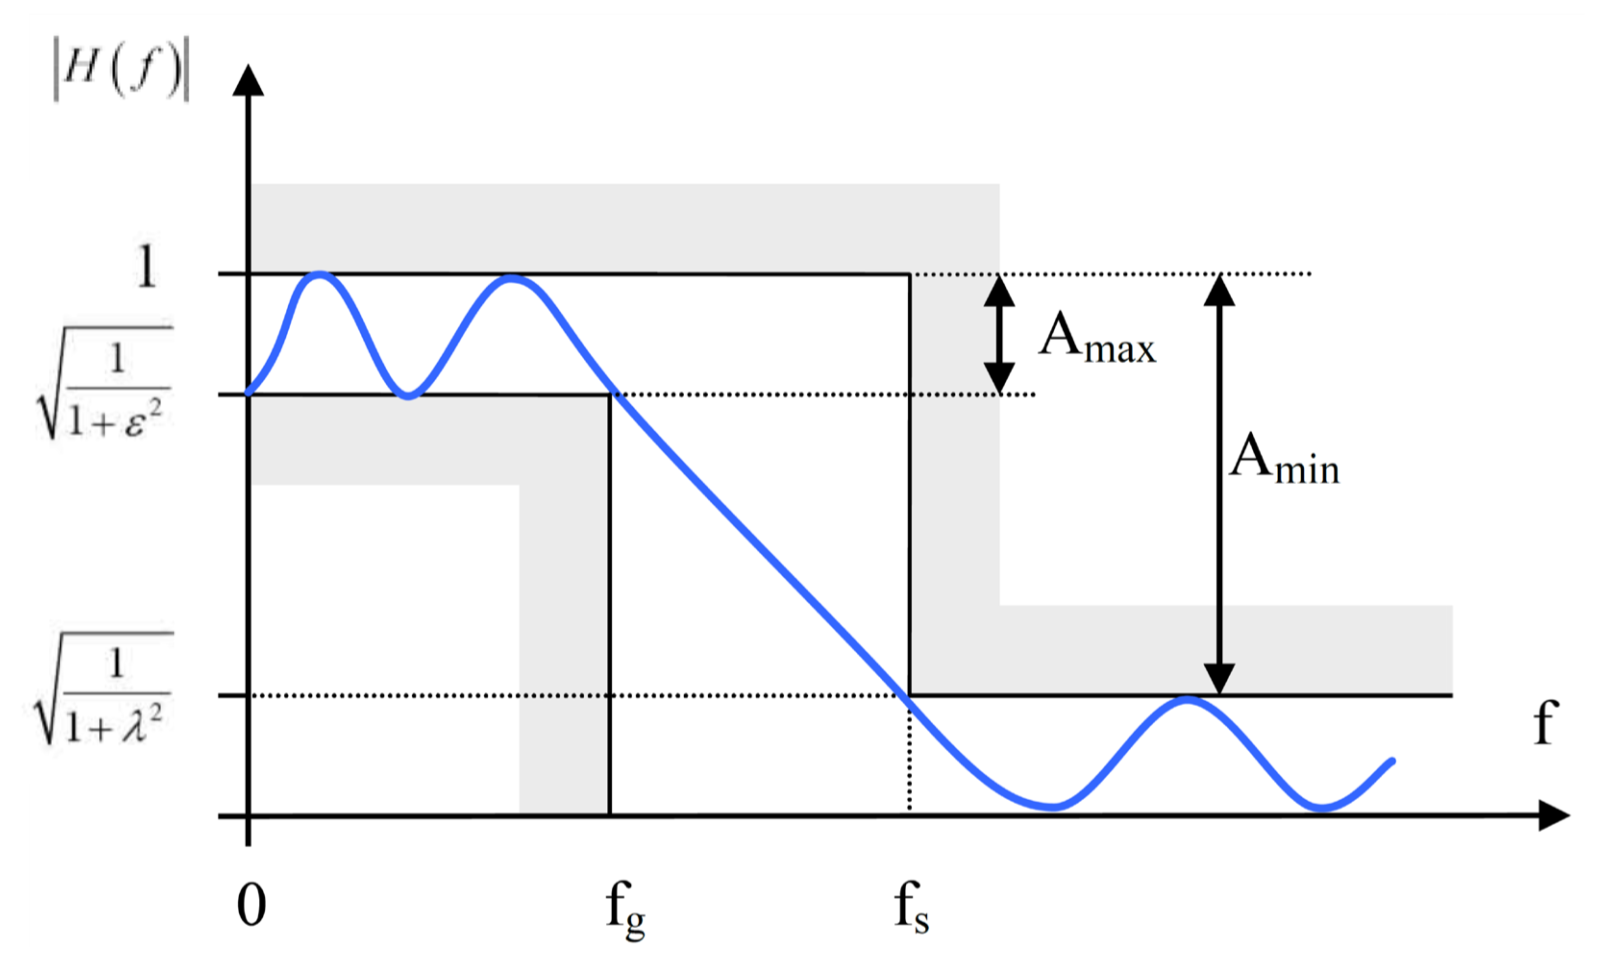
\includegraphics{images/03_Filtermaske.png}

}

\caption{Filtermaske eines Tiefpassfilters}

\end{figure}

Zur definition von Filtern gibt es verschiedene Approximationsverfahren

\begin{figure}[H]

{\centering 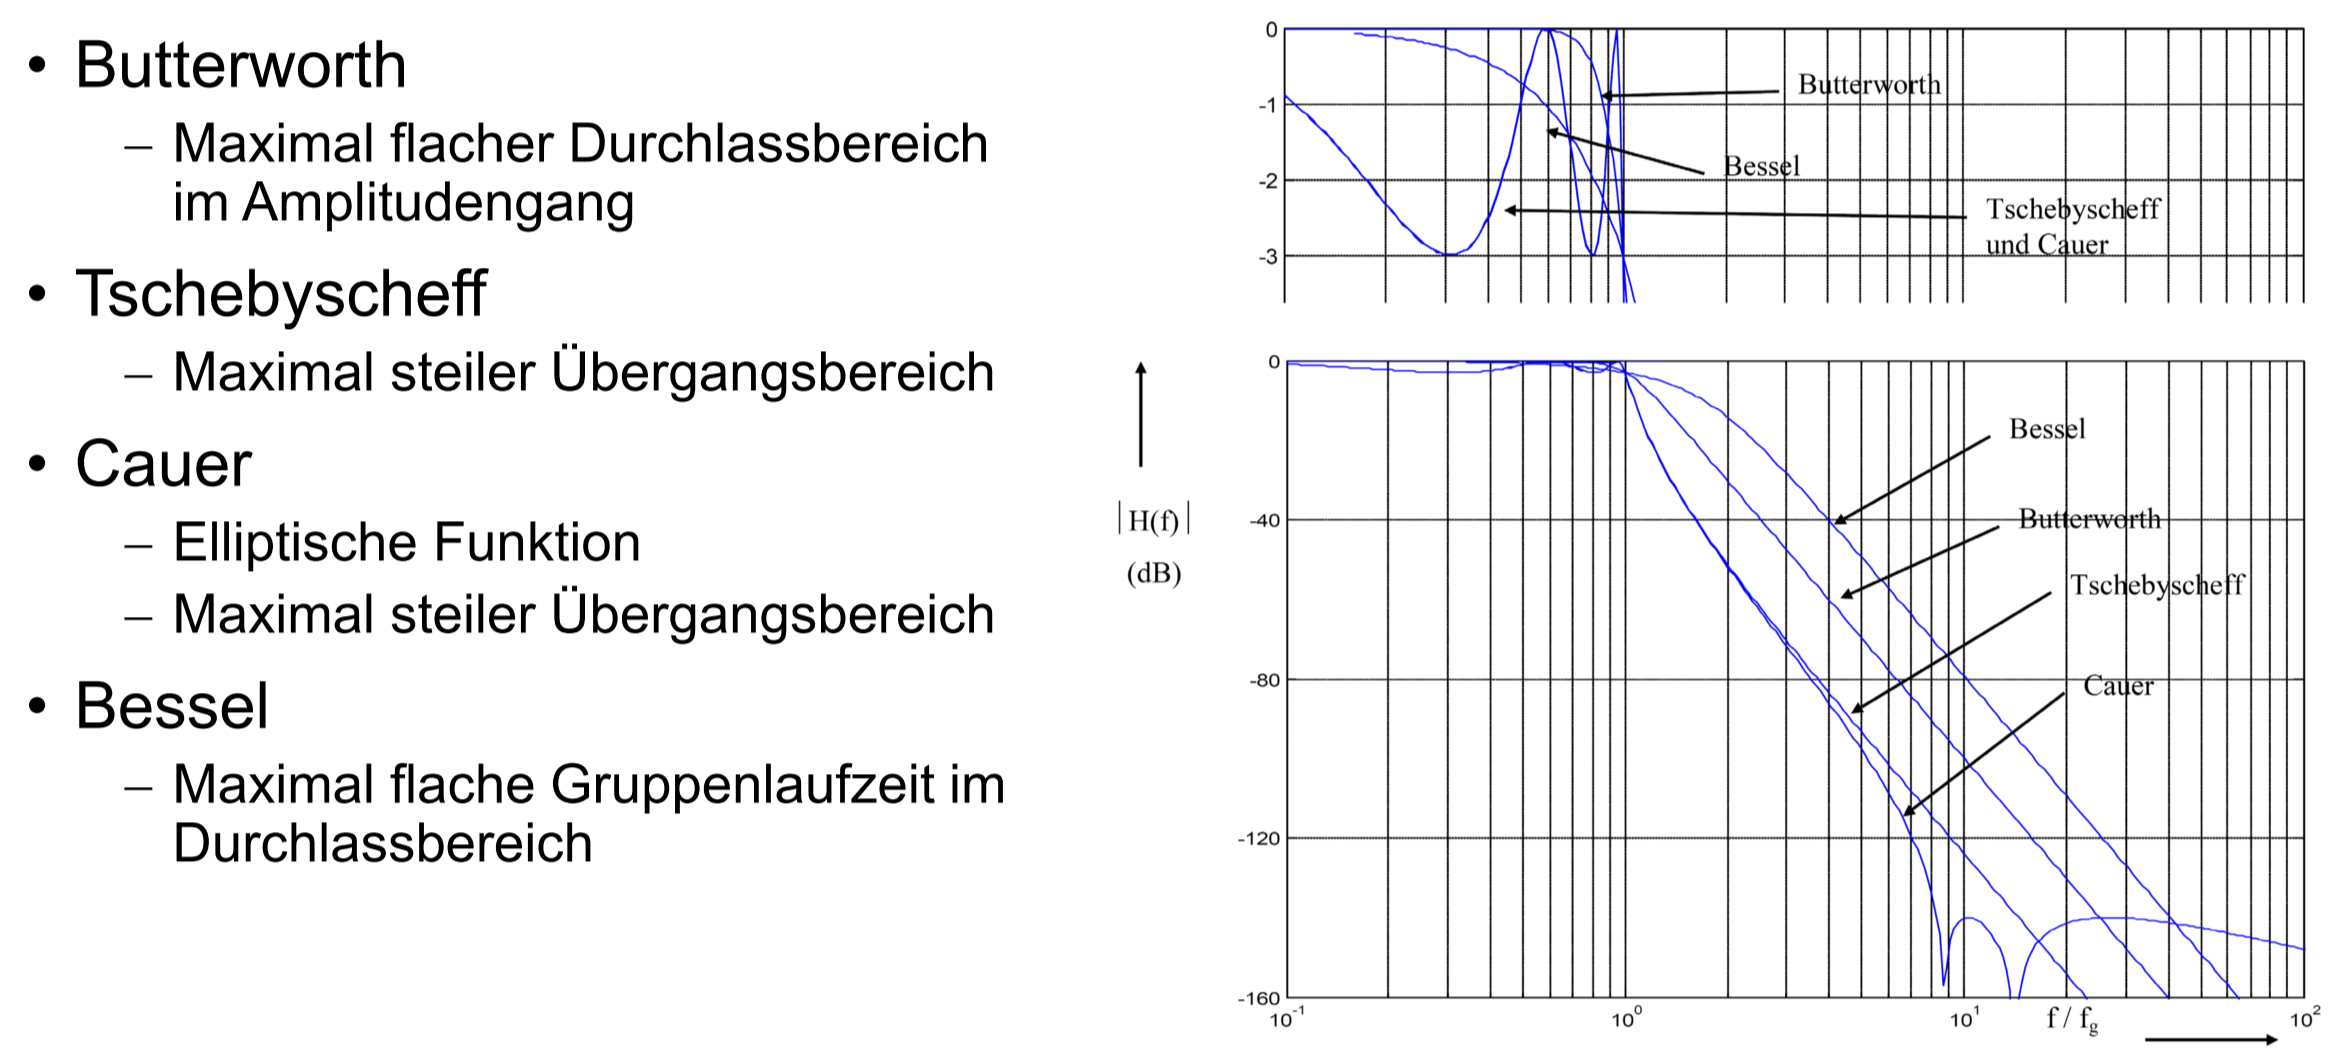
\includegraphics{images/03_Approximationsverfahren.png}

}

\caption{Aproximationsverfahren für Filterordnung \(n=5\) und
\(A\_{max}=3dB\)}

\end{figure}

\hypertarget{leitergebundene-uxfcbertragung}{%
\subsection{Leitergebundene
Übertragung}\label{leitergebundene-uxfcbertragung}}

Zur bestimmung ob ein Leiter mit der klassichen Schaltungstheorie oder
mit Phänomenen der elektromagnetischen welle betrachtet werden muss,
wird der Begriff der elektrischen Länge verwendet

\begin{figure}[H]

{\centering 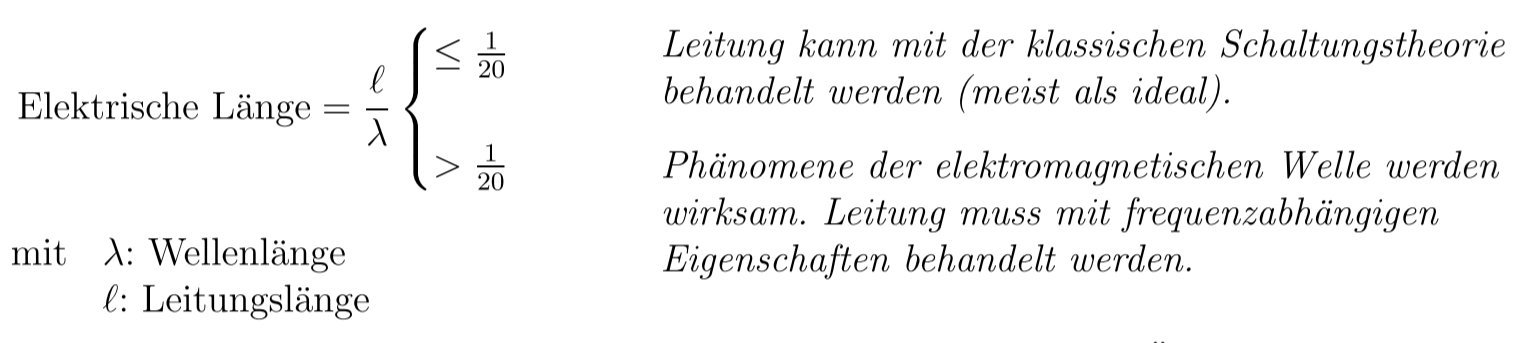
\includegraphics{images/03_ElektrischeLange.png}

}

\end{figure}

Wobei die Wellenlänge \(\lambda\) über die Geschwindigkeit \(v\) der
Signalwelle \emph{(max} \(v_0=3\cdot10^8\frac{m}{s}\)\emph{)} im
Übertragungsmedium mit der Frequenz \(f\) verbunden definiert ist durch

\[
\lambda=\frac{c}{f}\ [m]
\]

Längshomogene Zweidrahtleitungen aus metallischen Leitern können als
Zweitorkette modeliert werden

\begin{figure}[H]

{\centering 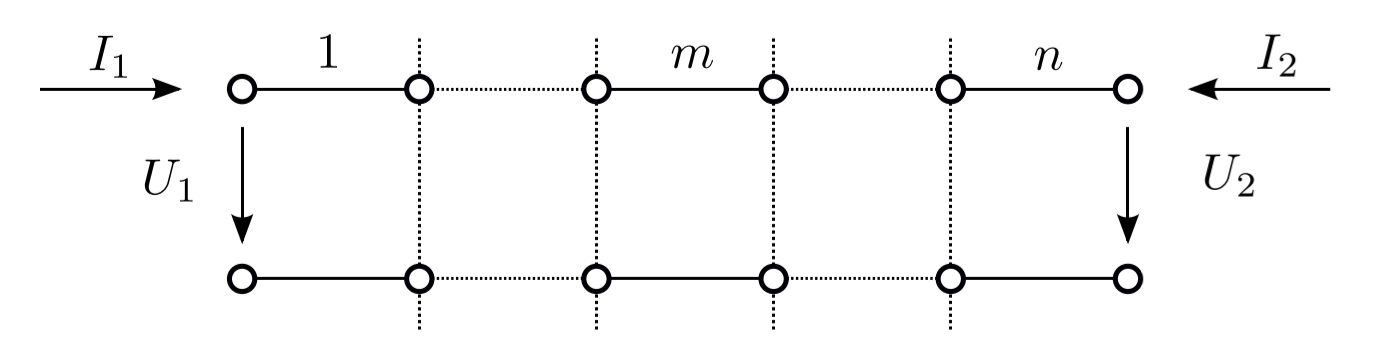
\includegraphics[width=14cm,height=\textheight]{images/03_Zweitorkette.png}

}

\end{figure}

Wird dabei die Weglänge \(\Delta z=\frac{1}{n}\) betrachtet so kann
angenommen werden, dass die Längsinduktivität \(\Delta L\) und die
Parallelkapazität \(\Delta C\) gleichförmig über die Länge \(\Delta z\)
verteilt sind. Diese werden in diesem Modell als \textbf{Leitungsbeläge}
ausgedrückt

\[
L'=\frac{\Delta L}{\Delta z}=\frac{L_l}{l}\ \left[\frac{H}{m}\right]\qquad\text{und}\qquad C'=\frac{\Delta C}{\Delta z}=\frac{C_l}{l}\ \left[\frac{F}{m}\right]
\]

Werden desweiteren ohmsche Verluste und dielektrische Verluste
dargestellt, so erhält man das Ersatzschaltbild einer Leitung

\begin{figure}[H]

{\centering 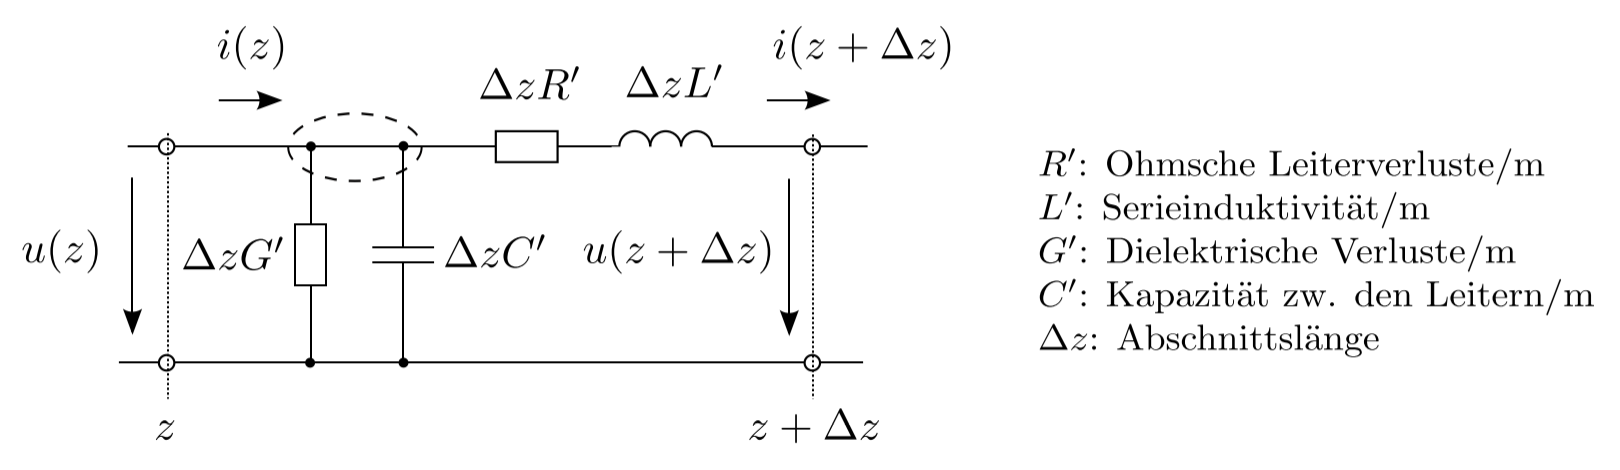
\includegraphics[width=15cm,height=4.3cm]{images/03_Leitung.png}

}

\end{figure}

Durch den Grenzwertübergang \(\Delta z\rightarrow 0\) erhält man die
\textbf{Telegraphengleichung}

\[
\frac{dI(z)}{dz}=-U(z)(G'+j\omega C')\qquad\text{und}\qquad\frac{dU(z)}{dz}=-I(z)(R'+j\omega L')
\]

Durch gegenseitiges einsetzten erhält man die \textbf{Wellengleichung}

\[
\frac{d^2I(z)}{dz^2}=\gamma^2I(z)\qquad\text{und}\qquad\frac{d^2U(z)}{dz^2}=\gamma^2U(z)
\]

mit der \textbf{komplexen Ausbreitungskonstante}

\[
\gamma=\alpha+j\beta=\sqrt{(R'+j\omega L')(G'+j\omega C')}
\]

\begin{conditions}
  \alpha & Dämpfungsbelag in $\left[\tfrac{Neper}{m}\right]$ (\textit{Neper} ist ein altes Dämpfungsmass) \\
  \beta & Phasenbelag in $\tfrac{rad}{m}$
\end{conditions}

\(\beta\) kann als Positionsabhängige Phasenverschiebung betrachtet
werden.

Die allgemeinen Lösungen der Wellengelichungen lauten \emph{(}\(_V\)
\emph{vorwärts laufend,} \(_R\) \emph{rückwärts laufend)}

\[
U(z,t)=(U_Ve^{-\gamma z}+U_Re^{\gamma z})e^{j\omega t}
\]

\[
I(z,t)=(I_Ve^{-\gamma z}+I_Re^{\gamma z})e^{j\omega t}
\]

Die Wellenfront bewegt sich mit der Ausbreitungsgeschwindigkeit
(\emph{propagation velocity}):

\[
v=\frac{2\pi f}{\beta} = \frac{\omega}{\beta}
\]

\[
\text{Freiraum}:\ \lambda_0=\frac{v}{f}=\frac{c_0}{f} \qquad \text{Material}:\ \lambda = \frac{v}{f}
\]

\begin{conditions}
  c_0,\,c & Lichtgeschwindigkeit ($299'792'458 \tfrac{m}{s}$)
\end{conditions}

Umrechnung der Spannungsreduktion von \emph{Neper} \(Np\) in
\emph{Dezibel} \(dB\) erfolgt durch

\[
\alpha_{dB/m}=10\cdot\log_{10}(r)\cdot\alpha_{Np/m}=20\cdot log_{10}(e)
\cdot\alpha_{Np/m}
=8.686\cdot\alpha_{Np/m}
\]

Die Welle hat also eine exponentiel abfallende Form

\begin{figure}[H]

{\centering \includegraphics[width=12cm,height=\textheight]{images/03_gedämpfteSchwinung.png}

}

\end{figure}

\hypertarget{charakteristische-leitungsimpedanz-z_0}{%
\subsubsection{\texorpdfstring{Charakteristische Leitungsimpedanz
\(Z_0\)}{Charakteristische Leitungsimpedanz Z\_0}}\label{charakteristische-leitungsimpedanz-z_0}}

\[
Z_0=\frac{U(z,t)}{I(z,t)}=\sqrt{\frac{Z'}{Y'}}=\sqrt{\frac{R'+j\omega L'}{G'+j\omega C'}}
\]

\hypertarget{leistungsfluss}{%
\subsubsection{Leistungsfluss}\label{leistungsfluss}}

Die Elektrische Leistung in der \emph{Vorwärtswelle} wird mit den
Effektivwerten berechnet

\[
P_v=\frac{U_VI_V^*}{2}=\frac{|U_V|^2}{2Z_0}
\]

Für die \emph{Rückwertswelle} wechselt das Vorzeichen der
charakteristischen Impedanz und somit die Richtung des Leistungsflusses

\[
P_R=\frac{U_RI_R^*}{2}=-\frac{|U_R|^2}{2Z_0}
\]

\hypertarget{leitergeometrien}{%
\subsubsection{Leitergeometrien}\label{leitergeometrien}}

Verschiedene Leitergometrien führen zu unterschiedlichen Impedanzen und
Belägen

\begin{figure}[H]

{\centering 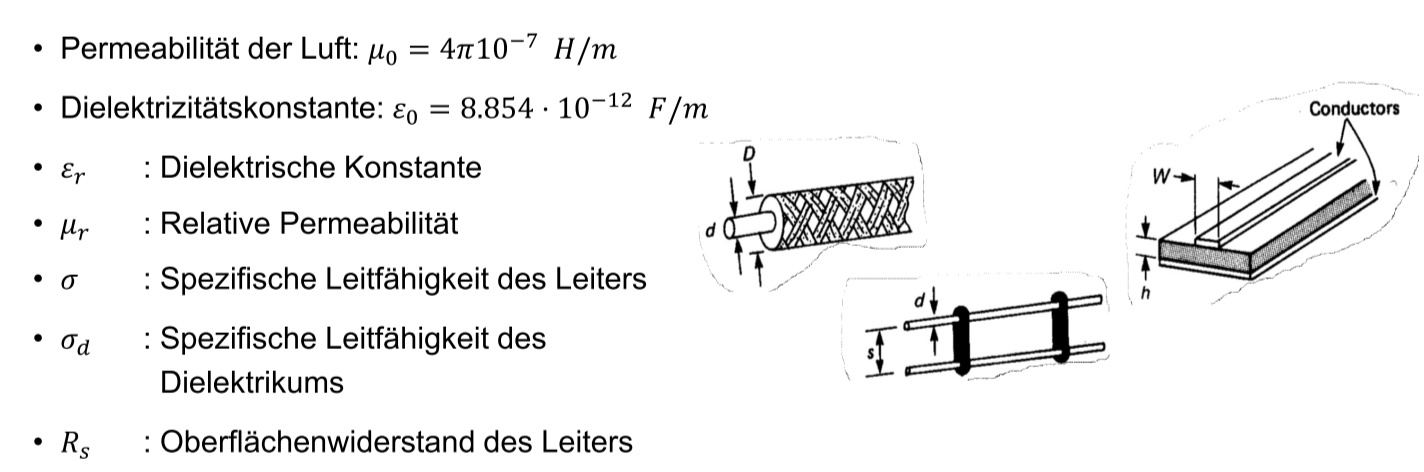
\includegraphics{images/03_leiterimpedanzen.png}

}

\end{figure}

Wobei der Oberflächenwiderstand allgmein als

\[
R_S=\sqrt{\frac{\pi\mu_{Leiter}f}{\sigma_{Leiter}}}
\]

definiert ist. Die unterschiedlichen Belagsgrössen sind abhängig von der
Leitergeometrie

\begin{figure}[H]

{\centering 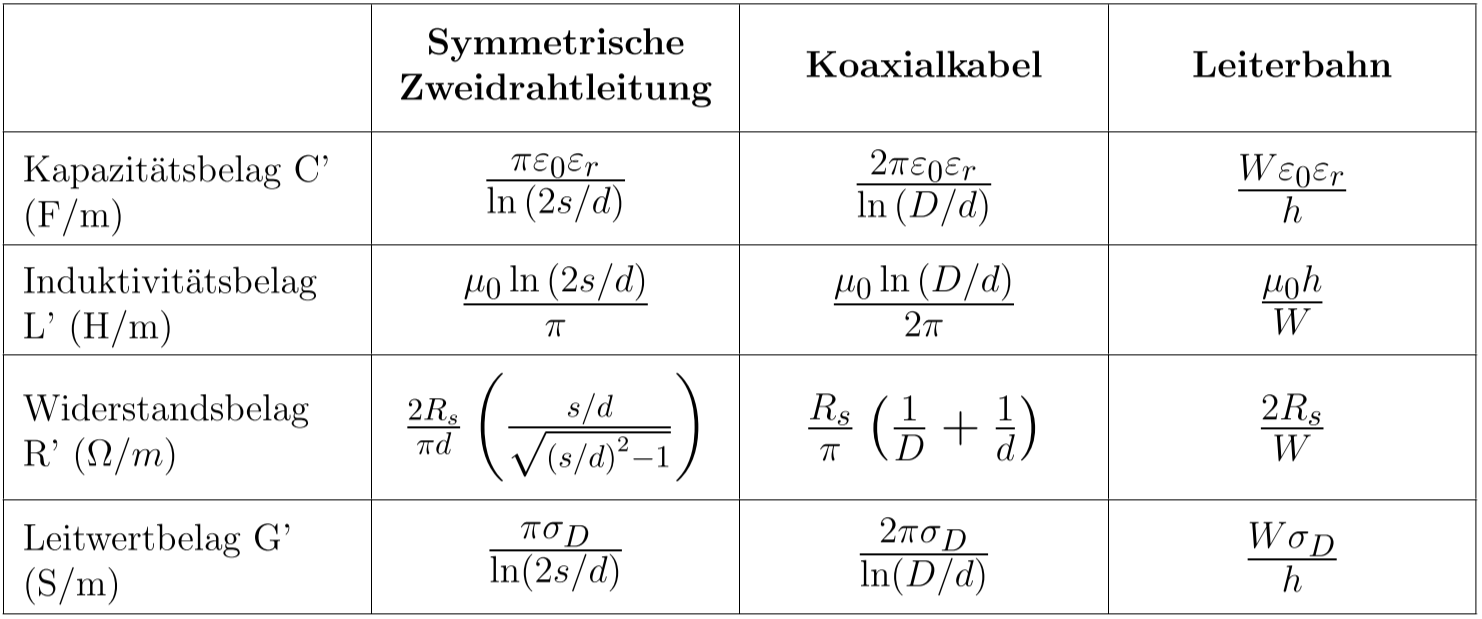
\includegraphics{images/03_Belagsgroessen.png}

}

\end{figure}

\hypertarget{reflexionen-an-der-last}{%
\subsubsection{Reflexionen an der Last}\label{reflexionen-an-der-last}}

Entspricht die \emph{Lastimpedanz} \(Z_L\) nicht der Leitungsimpedanz
\(Z_0\) so entsteht eine \textbf{Stosswelle} am Übergang. Es kommt zu
einer (Teil-)Reflexion der vorlaufenden Signalwelle. Es wird eine neue
rücklaufende Signalwelle erzeugt.

\begin{figure}[H]

{\centering 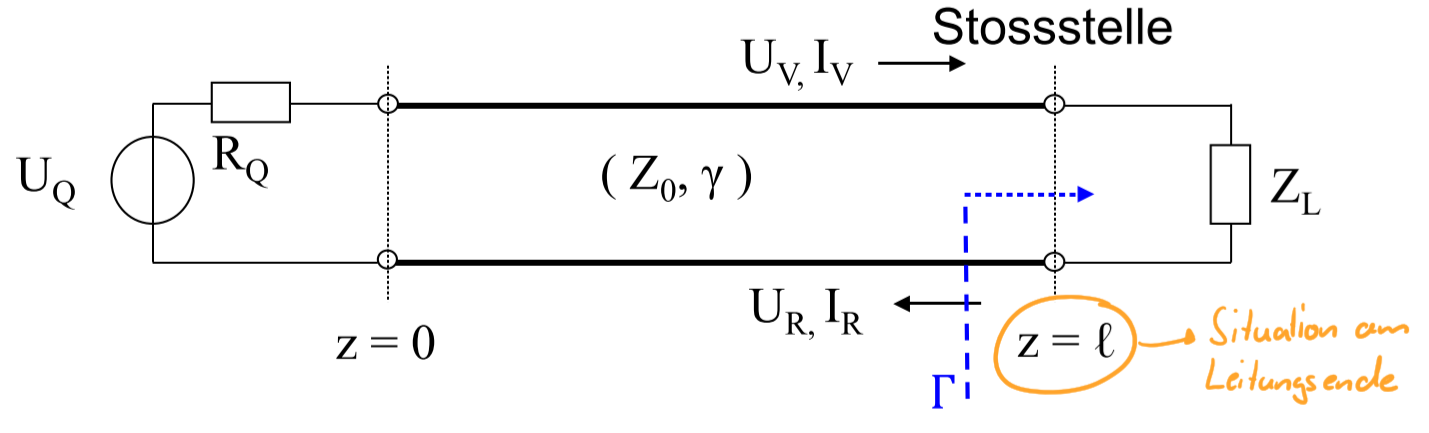
\includegraphics[width=14cm,height=\textheight]{images/03_Reflexion.png}

}

\end{figure}

Das Verhältnis der Vor- und Rücklaufenden Amplituden bildet den
\textbf{Reflexionskoeffizient}

\[
\Gamma_{z=\ell}=\frac{Z_L-Z_0}{Z_L+Z_0}=\frac{U_R}{U_V}=-\frac{I_R}{I_V}
\]

\begin{conditions}
  \Gamma_{z=l} & Reflexionskoeffizient $\rightarrow$ je näher an Null, desto besser.
\end{conditions}

\begin{tcolorbox}[enhanced jigsaw, breakable, colback=white, opacityback=0, leftrule=.75mm, colframe=quarto-callout-note-color-frame, left=2mm, bottomrule=.15mm, toprule=.15mm, rightrule=.15mm, arc=.35mm]
\begin{minipage}[t]{5.5mm}
\textcolor{quarto-callout-note-color}{\faInfo}
\end{minipage}%
\begin{minipage}[t]{\textwidth - 5.5mm}

\textbf{Spezialfälle \(Z_L\)}\vspace{2mm}

\begin{itemize}
\item
  \(Z_L = 0\Omega\ \Rightarrow\ \Gamma=-1\quad\rightarrow\quad U_{ZL}=0,\, I_{ZL}=2\cdot I_V\)
\item
  \(Z_L=\infty\ \Rightarrow\ \Gamma=+1\quad\rightarrow\quad U_{ZL}=2\cdot U_V,\, I_{ZL}=0\)
\item
  \(Z_L=Z_0\ \Rightarrow\ \Gamma=0\quad\rightarrow\quad U_{ZL}=U_V,\, I_{ZL}=I_V\)
\end{itemize}

\end{minipage}%
\end{tcolorbox}

Der Wertebereich von \(\Gamma\) liegt innerhalb des Einheitskreises der
komplexen Ebene

\begin{figure}[H]

{\centering 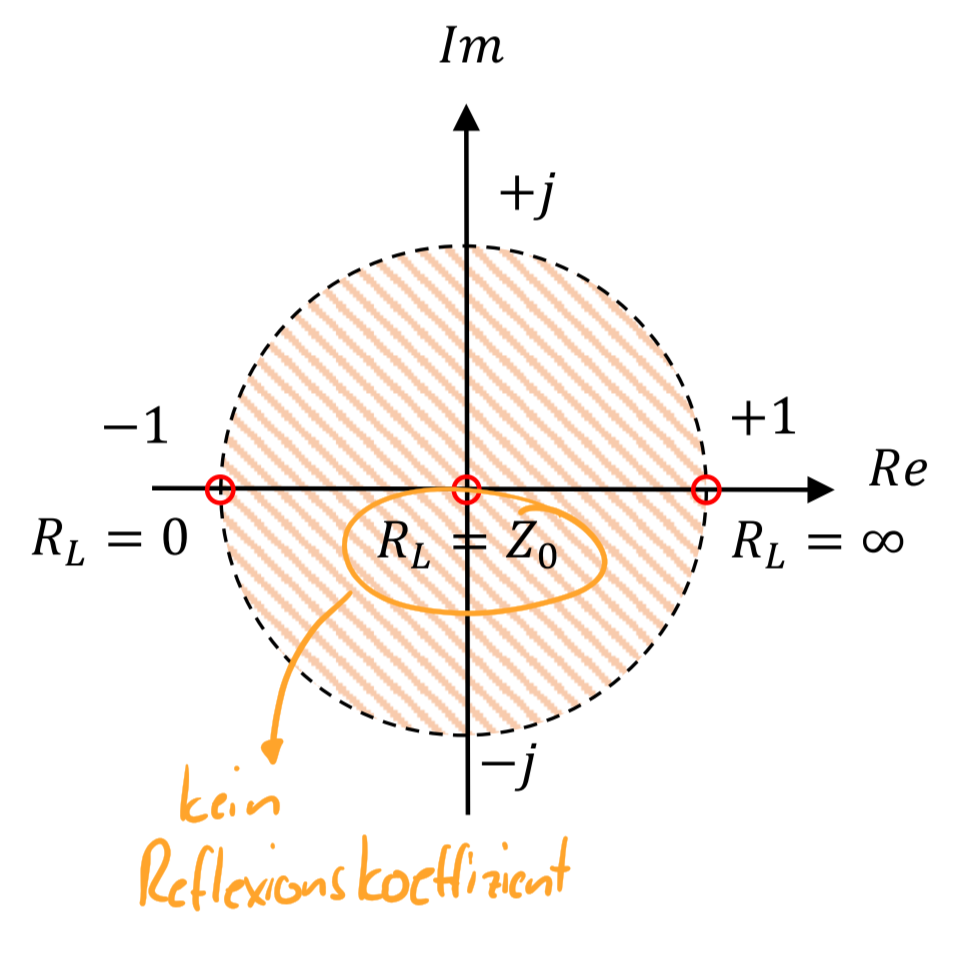
\includegraphics[width=9cm,height=\textheight]{images/03_Reflexionskoeffizient.png}

}

\end{figure}

Die resultierende Spannung und Strom auf der Leitung ist die
Überlagerung von vor- und rücklaufenden Signalwellen

\[
U(z)=U_V\cdot e^{-\gamma z}+U_Re^{-\gamma(\ell-z)}=U_V\cdot e^{-\gamma z}(1+\Gamma_Le^{-2\gamma(\ell-z)})
\]

\[
I(z)=I_V\cdot e^{-\gamma z}+I_Re^{-\gamma(\ell-z)}=\frac{U_V\cdot e^{-\gamma z}}{Z_0}(1+\Gamma_Le^{-2\gamma(\ell-z)})
\]

Der Reflexionskoeffizient entlang der Leitung entspricht

\[
\Gamma(z)=\Gamma_L e^{-2\gamma(\ell-z)}
\]

Die Impedanz auf der Leitung an einem beliebigen Punkt \(z\) entspricht

\[
Z(z)=\frac{U(z)}{I(z)}=Z_0\frac{Z_L+Z_0\tanh(\gamma(\ell-z))}{Z_0+Z_L\tanh(\gamma(\ell-z))}
\]

und bei einer \ul{verlustlosen} Leitung

\[
Z(z)=\frac{U(z)}{I(z)}=Z_0\frac{Z_L+jZ_0\tan(\beta(\ell-z))}{Z_0+jZ_L\tan(\beta(\ell-z))}
\]

\hypertarget{welligkeitsfaktor}{%
\subsubsection{Welligkeitsfaktor}\label{welligkeitsfaktor}}

Die Überlagerungen der vor- und rücklaufenden Welle bildet örtliche
Maxima und Minima, was zu einer stehenden Welle führt. Der
Welligkeitsfaktor ist definiert durch

\[
s=\frac{\hat{U}_{max}}{\hat{U}_{min}}=\frac{|U_V|+|U_R|}{|U_V|-|U_R|}=\frac{1+|\Gamma|}{1-|\Gamma|}
\]

Die Rückflussdämpfung bezeichnet wie viel das rücklaufende Signal
gegenüber dem vorlaufenden gedämpft ist

\[
a=-\log_{10}(|\Gamma|^2)
\]

Die Überlagerungen führen zu einer Hüllkurve

\begin{figure}[H]

{\centering \includegraphics{images/03_Hüllkurve.png}

}

\end{figure}

\begin{equation}\protect\hypertarget{eq-test}{}{
P_L=P_V(1-|\Gamma|^2)
}\label{eq-test}\end{equation}

\begin{tcolorbox}[enhanced jigsaw, toptitle=1mm, breakable, colback=white, opacityback=0, colframe=quarto-callout-important-color-frame, bottomrule=.15mm, toprule=.15mm, bottomtitle=1mm, opacitybacktitle=0.6, coltitle=black, leftrule=.75mm, left=2mm, colbacktitle=quarto-callout-important-color!10!white, rightrule=.15mm, titlerule=0mm, title=\textcolor{quarto-callout-important-color}{\faExclamation}\hspace{0.5em}{Maximale Wirkleistungsübertragung}, arc=.35mm]

Die maximale Wirkleistungsübertragung von der Leitung zur Last kann nur
erreicht werden, wenn \(Z_0\) und \(Z_L\) reell und gleich gross sind.

\end{tcolorbox}

\hypertarget{ausgleichsvorgang-an-einer-stossstelle}{%
\subsubsection{Ausgleichsvorgang an einer
Stossstelle}\label{ausgleichsvorgang-an-einer-stossstelle}}

Die Verzögerung durch die Phasengeschwindigkeit des Leiters führt zu
einem \emph{verspäteten} Signalverlauf am anderen Ende des Leiters, dies
wird mit der Laufzeit \(t_d\) dargestellt:

\[
t_d = \frac{l}{v}=\frac{\beta\cdot l}{\omega}
\]

Hat es unterschiedliche Impedanzen (Leiter-, Innen-, Lastimpedanz), kann
es zu einem \emph{Einschwingen} des Signales führen. Grund dafür sind
die Reflektionen des Leiters, welches Stücke des Signals hin und her
reflektiert, bis es den entsprechenden Wert erreicht.

\begin{figure}[H]

{\centering 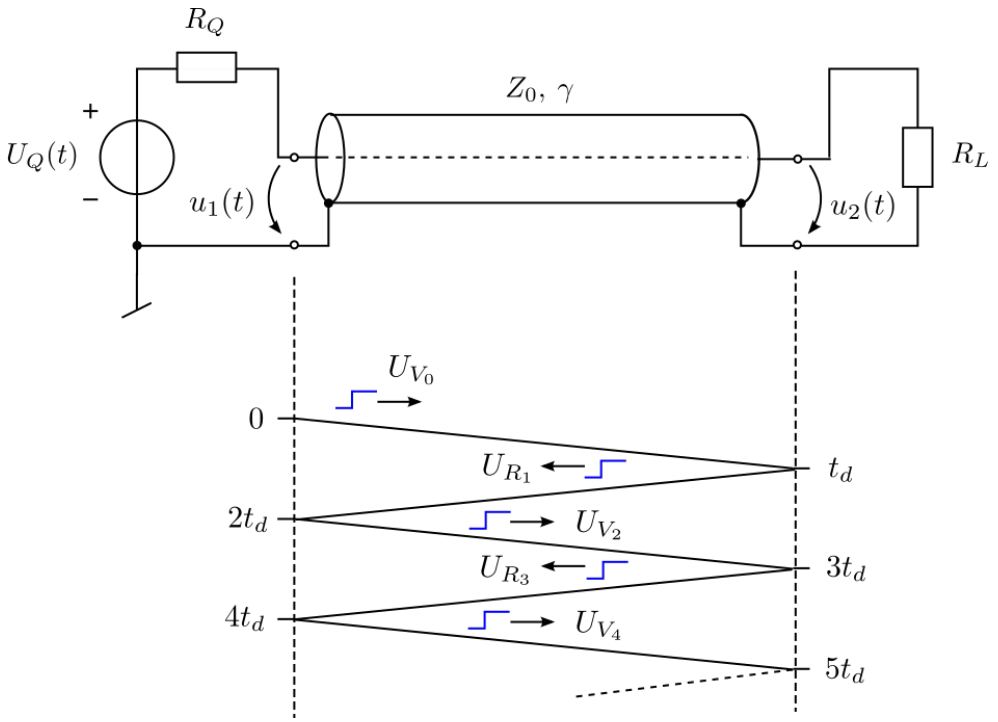
\includegraphics[width=12cm,height=\textheight]{images/03_Ausgleichsvorgang.png}

}

\end{figure}

\begin{multicols}{2}

Beide Enden des Leiters haben je einen Reflexionskoeffizienten:
\(\Gamma_1\) für den Anfang des \ul{Leiters} (aus Sicht der Quelle) und
\(\Gamma_2\) für das Ende.

\[
\Gamma_1 = \frac{R_Q-Z_0}{R_Q+Z_0} \qquad \Gamma_2 = \frac{R_L-Z_0}{R_L+Z_0}
\]

Die Spannungen \(u_1(t)\) \& \(u_2(t)\) an den beiden Enden des Leiters
entsprechen der Aufsummierungen der Reflexionsspannungen.

\[
u_1(t)=\sum U_i \qquad u_2(t)=\sum U_i
\]

Zu Beginn wird das Signal von \(U_Q=1\text{V}\) angelegt und es dauert
\(1\cdot t_d\) bis die Spannung \(U_{V_0}\) das Ende des Leiters
erreicht.

\[
U_{V_0} = U_Q \cdot \frac{Z_0}{R_Q+Z_0}
\]

Da die Leiter- \& Lastimpedanz unterschiedlich ist, wird das Signal mit
dem Faktor \(e^{-\gamma\cdot l}\cdot \Gamma_2\), wobei in diesem
Beispiel mit \(\gamma=0\) gerechnet wird.

\[
U_{R_1}=U_{V_0}\cdot e^{-\gamma\cdot l}\cdot \Gamma_2
\]

Wird zum Zeitpunkt \(1\cdot t_d\) die Spannung \(u_2(t)\) mit einem
Oszilloskop gemessen, misst man
\(u_2(t_d)=U_{V_0}+U_{R_1}=\tfrac{4}{3}\text{V}\). Da auch die Innen- \&
Leiterimpedanz unterschiedlich sind, reflektiert das Signal mit dem
Faktor \(e^{-\gamma\cdot i}\cdot \Gamma_2\) zurück. Dies wiederholt
sich, bis die Spannung eingeschwungen ist.

\[
U_{V_2}=U_{R_1}\cdot e^{-\gamma\cdot l}\cdot \Gamma_1
\]

\end{multicols}

Folgend zeigt eine ``Messung'' von \(u_2(t)\) mit folgenden
Widerstandswerten:
\(R_Q=0\Omega,\, Z_0=50\Omega,\, R_L=100\Omega,\, l=1\text{m},\, v=0.5c_0\)

\begin{figure}[H]

{\centering 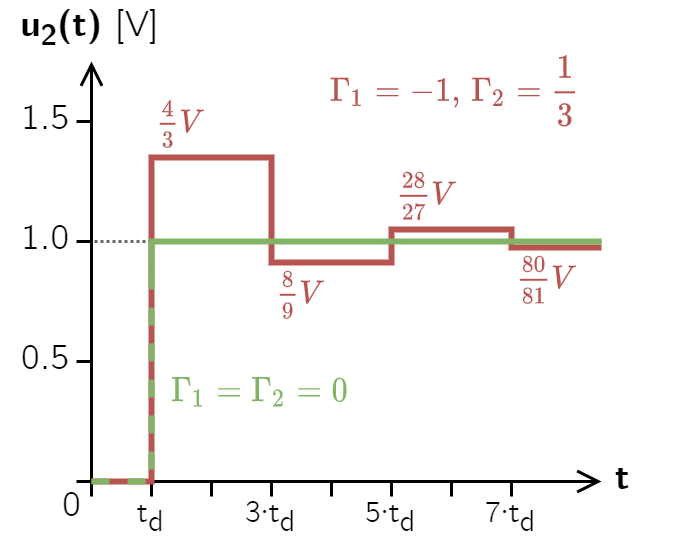
\includegraphics[width=8cm,height=\textheight]{images/03_ausgleichsvorgang_u2.png}

}

\caption{\label{fig-ausgleichsvorgang}Ausgleichsvorgang \(u_2(t)\)}

\end{figure}

\hypertarget{drahtlose-signaluxfcbertragung--filterung}{%
\section{Drahtlose Signalübertragung \&
-Filterung}\label{drahtlose-signaluxfcbertragung--filterung}}

\begin{figure}[H]

{\centering 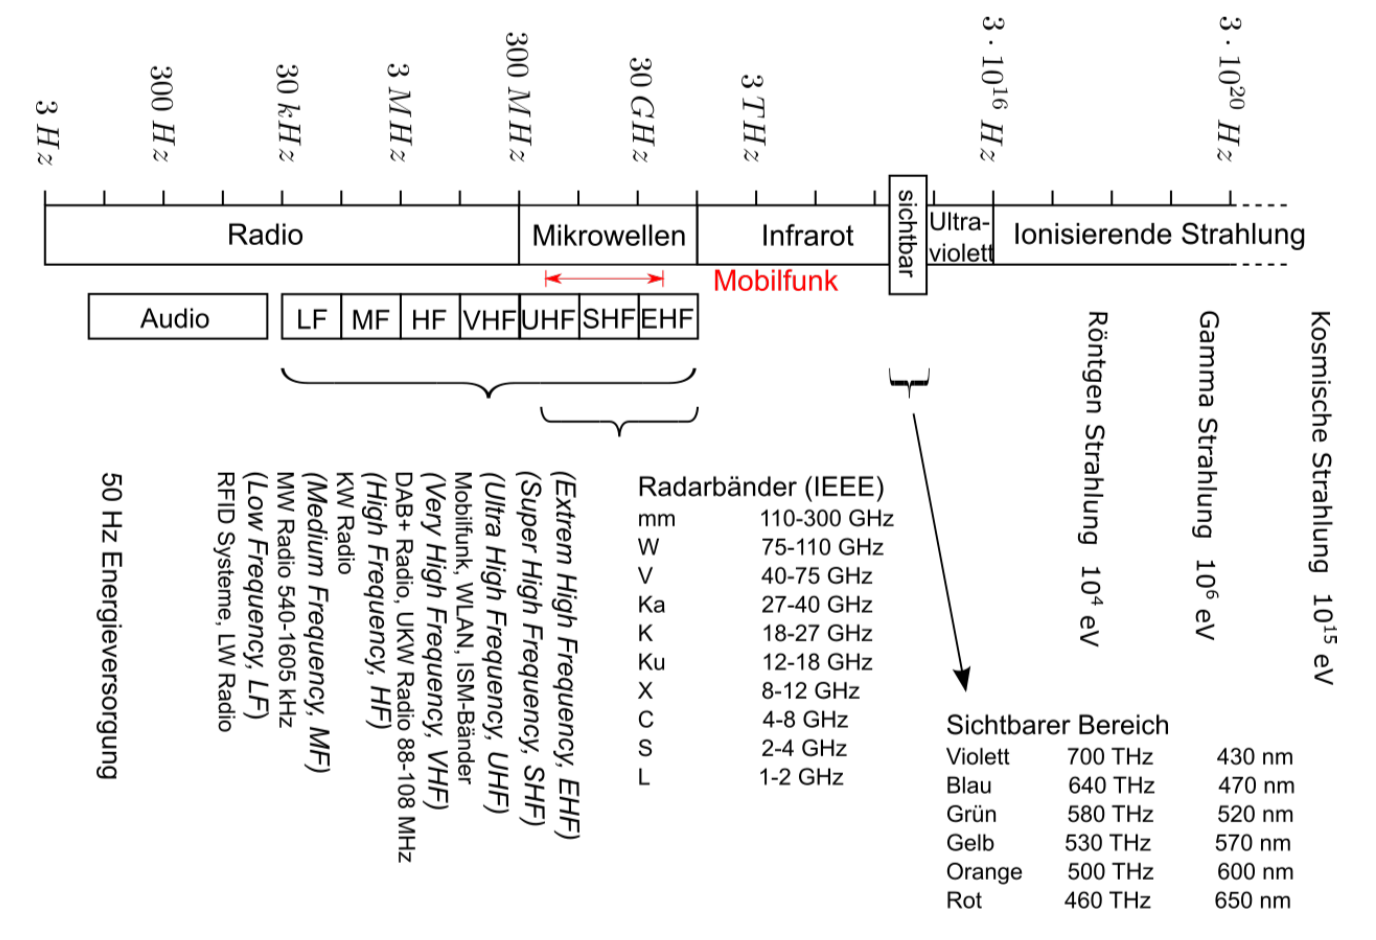
\includegraphics{images/04_Spektrumsbereich.png}

}

\caption{Spektrumsbereich}

\end{figure}

Es gibt verschiedene Ausbreitungsarten, welche zum Teil auch vom
Spektrum abhängen

\begin{itemize}
\item
  \emph{Bodenwelle} breitet sich entlang der ``Materialgrenze''
  Luft-Boden aus
\item
  \emph{Direktverbindung} (auch \emph{Line-of-Sight} oder \emph{free
  space propagation}) im nicht ionisierenden Bereich der Atmosphäre
\item
  \emph{Raumwelle} erfolgt durch die Reflektion am ionisierten Bereich
  der Atmosphäre, ab ca. \textbf{100MHz} durchdringen Wellen die
  Ionosphäre

  \begin{figure}[H]

  {\centering 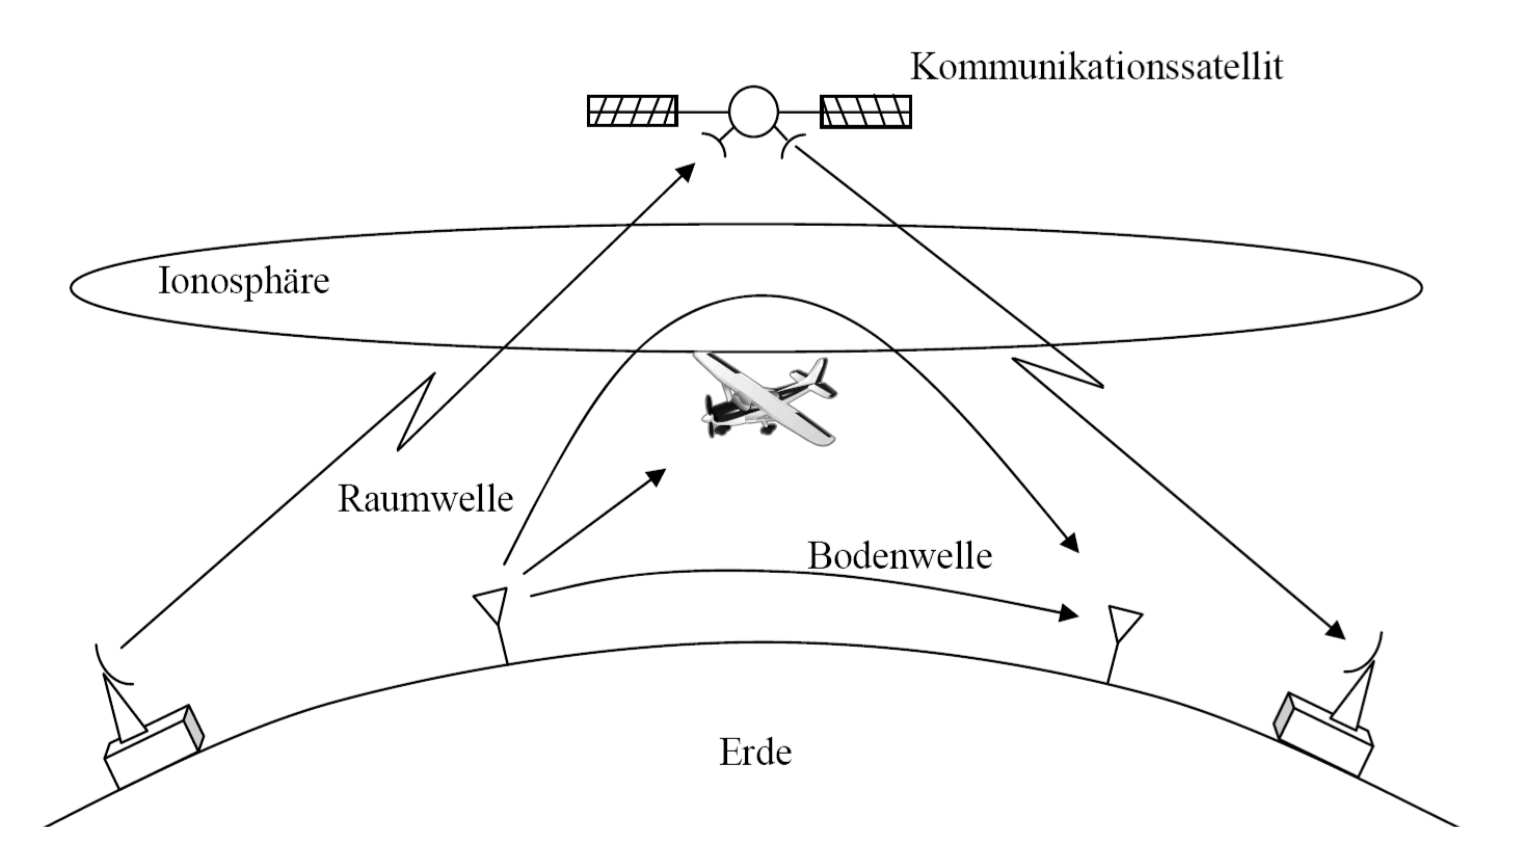
\includegraphics{images/04_AusbreitungVonRadiowellen.png}

  }

  \end{figure}
\end{itemize}

\hypertarget{linkbudget}{%
\subsection{Linkbudget}\label{linkbudget}}

Beim Entwurf eines Übertragungssystems interessiert primär die Leistung
\(P_{Rx}\) am Empfängereingang. Diese ist jedoch abhängig von den
Verlusten und Gewinnen der Sender, Kabel, Antennen.

\begin{figure}[H]

{\centering 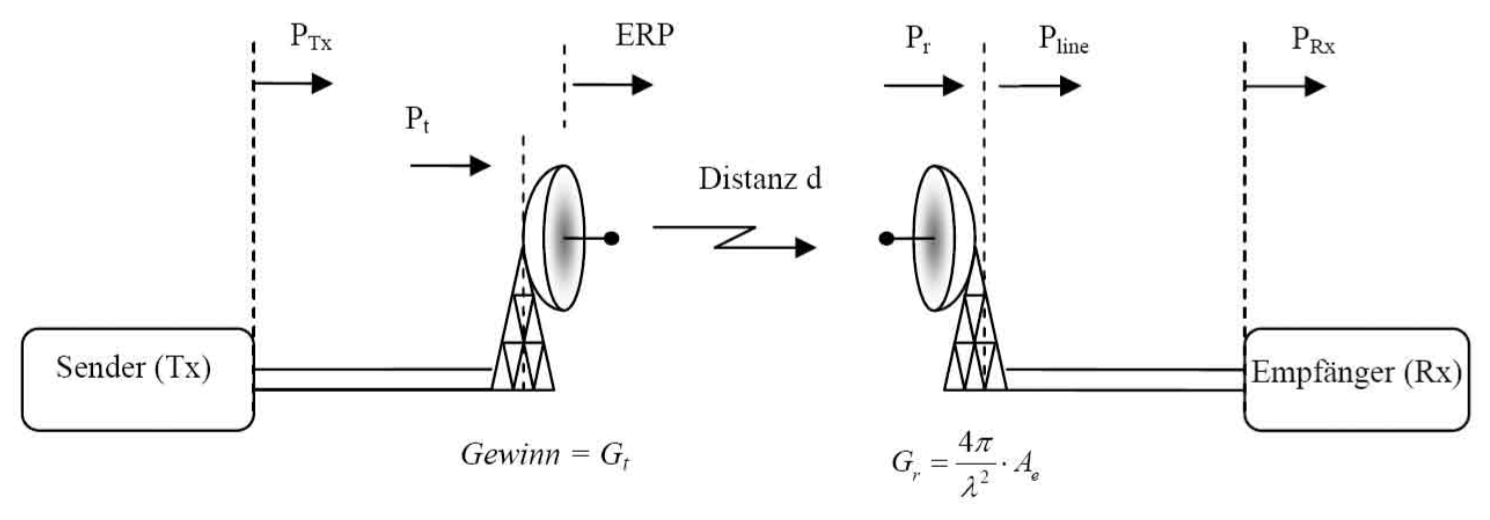
\includegraphics{images/04_DrahtloseUebertragung.png}

}

\end{figure}

Die Leistung am Empfänger kann also erhöht werden durch\ldots{}

\begin{itemize}
\item
  Sendeleistung \(P_{Tx}\) erhöhen
\item
  Verluste der Zubringerkabel minimieren
\item
  Reflexionen an den Übergängen minimieren
\item
  Sende- bzw. Empfangsgewinne \(G_t\) und \(G_r\) vergrössern
\end{itemize}

Die Empfangsleistung \(P_{Rx}\) muss dabei genügend gross sein, damit
das Signal mit einer guten Qualität am Empfängereingang vorliegt. Für
eine bessere Übersicht für einen \emph{Systementwurf} wird ein
Linkbudget aufgestellt

\begin{figure}[H]

{\centering 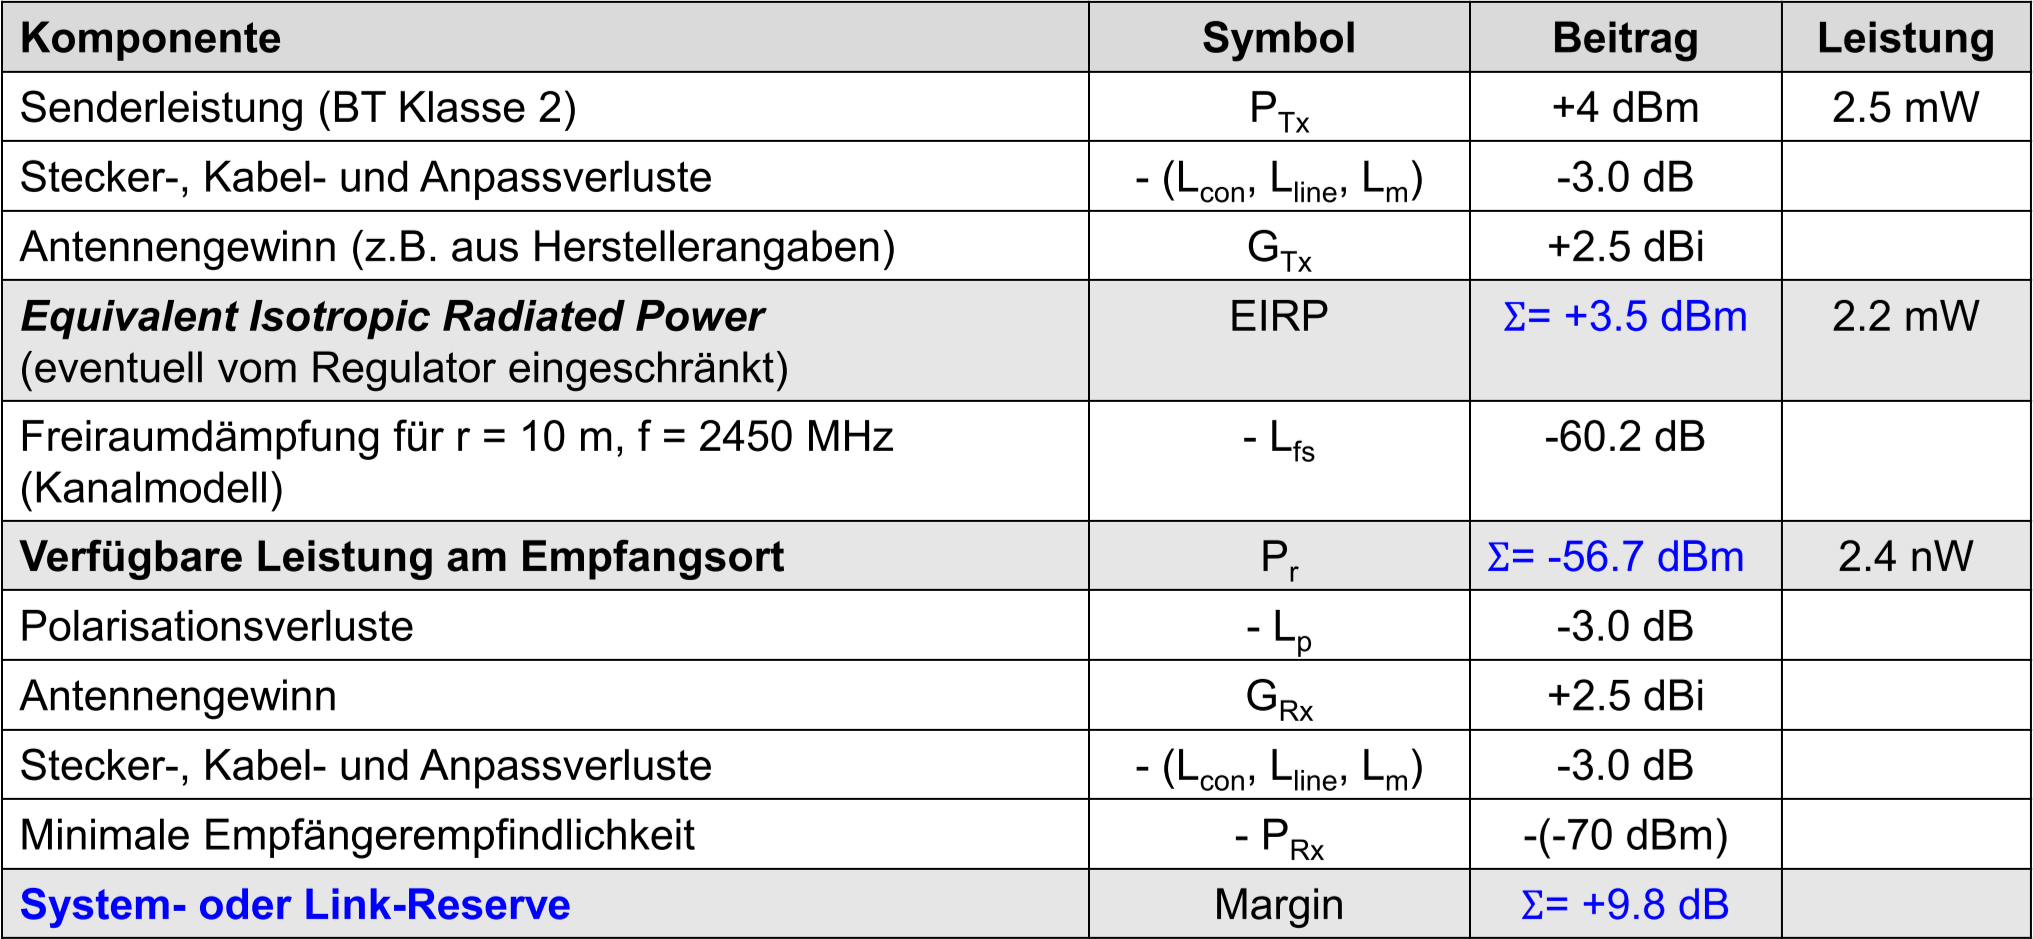
\includegraphics{images/04_Linkbudget.png}

}

\caption{Linkbudget einer Blutooth Verbindung \emph{(2.45 GHz)}}

\end{figure}

\hypertarget{antenne}{%
\subsection{Antenne}\label{antenne}}

\hypertarget{fernfeld-kriterien}{%
\subsubsection{Fernfeld Kriterien}\label{fernfeld-kriterien}}

Das Feld einer Antenne kann konzeptionell in ein \textbf{Nahfeld} und
ein \textbf{Fernfeld} aufgeteilt werden. Das \emph{Nahfeld} kann
nochmals in ein \textbf{reaktives} \emph{Nahfeld} und ein
\textbf{strahlendes} \emph{Nahfeld} unterteilt werden.

\begin{figure}[H]

{\centering 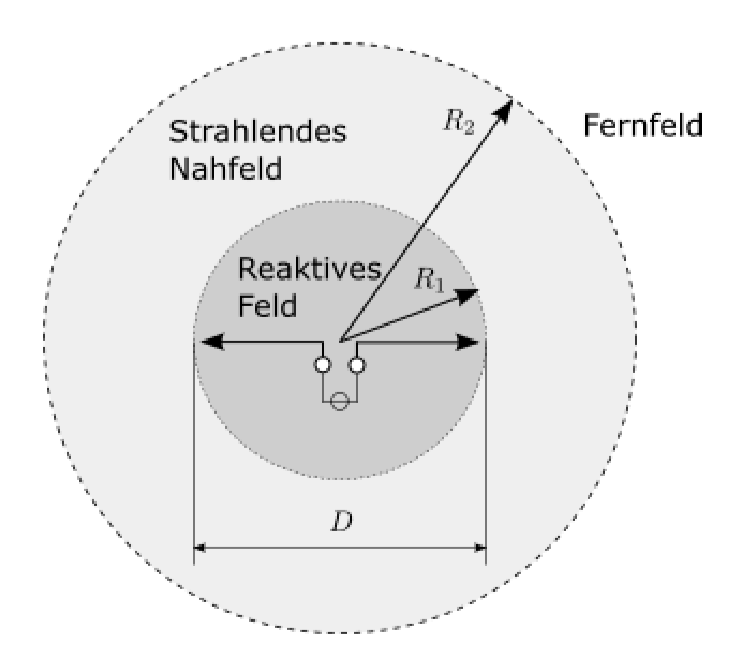
\includegraphics{images/04_Fernfeld.png}

}

\end{figure}

Im \textbf{Fernfeld} erscheint jede Antenne als \emph{Punktstrahler},
die Kugelform kann jedoch vernachlässigt werden und man nimmt für die
Ausbreitung eine \emph{ebene Wellenfront} an. Als \textbf{Fernfeld} gilt
der bereich ausserhalb \(R_2\) nach

\[
R_2=\frac{2D^2}{\lambda}\qquad\text{oder}\qquad R_2=1.6\lambda
\]

mit \(D\) als grösstes Antennenmass.

Der Übergangsbereich des \textbf{strahlenden} \emph{Nahfeldes} hat die
untere Grenze \(R_1\) mit

\[
R_1\approx 0.62\sqrt{\frac{D^3}{\lambda}}
\]

\hypertarget{antennenimpedanz}{%
\subsubsection{Antennenimpedanz}\label{antennenimpedanz}}

Antennen können Allgemein als Impedanzwandler zwischen dem Übertrager
\emph{(Schaltungstheorie)} \(Z_0\) und der Luft \emph{(Feldtheorie)}
\(Z_w=\frac{E}{H}\approx 377\Omega\) angesehen werden.

\begin{figure}[H]

{\centering 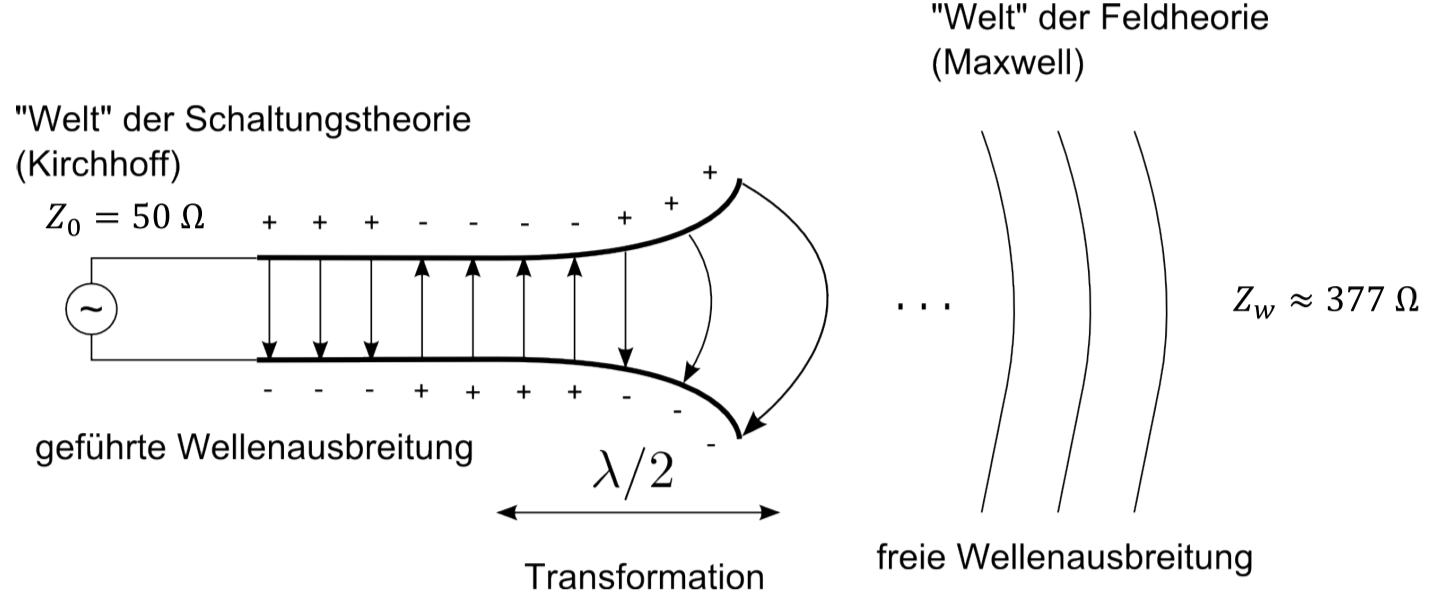
\includegraphics{images/04_Impedanzwandler.png}

}

\end{figure}

Die Antennenimpedanz \(Z_{ant}\) hängt direkt von der Antennengeometrie
ab und kann als Ersatzschaltung dargestellt werden

\begin{figure}[H]

{\centering \includegraphics{images/04_ErsatzschaltungImpedanz.png}

}

\end{figure}

Die Wichtigsten Eigenschaften sind hierbei

\begin{multicols}{2}

Die \textbf{Strahlungseffizienz} \(\eta\) ist definiert durch

\[
\eta=\frac{R_{rad}}{R_\Omega+R_{rad}}
\]

Wodurch auf den Antennengewinn \(G\) geschlossen werden kann

\[
G=D\cdot\eta
\]

Die abgegebene Leistung \(P_{ant}\) hängt direkt von der Anpassung von
Zubringerkabel und Antenne ab

\[
P_{ant}=P_t(1-|\Gamma|^2)\qquad\text{mit}\qquad\Gamma=\frac{Z_{ant}-Z_0}{Z_{ant}+Z_0}
\]

Die Reflexion beträgt dabei

\[
\Gamma_{dB}=10\log_{10}{(|\Gamma|^2}
\]

Die \emph{relative Bandbreite} \(B_r\) ist gegeben durch die
Mittenfrequenz \(f_0\) und die Bandbreite \(B\) bei \(xx\space dB\)

\[
B_r=\frac{B}{f_0}
\]

\columnbreak

\(Z_{ant}\) Antennenimpedanz und Anpassung

\(R_\Omega\) stellt die ohm'schen Verluste der Antennestruktur dar

\(R_{rad}\) entspricht der abgestrahlten \emph{Wirkleistung}

\(X_{ant}\) ist der Blindwiderstand, der vom \emph{reaktiven} Nahfeld
beeinflusst werden kann

\(D\) Richtwirkung \emph{(nicht} \(D\) \emph{als Antennenmass)}

\(G\) Antennengewinn

Polarisation

\(B\) Bandbreite

\end{multicols}

\begin{figure}[H]

{\centering \includegraphics{images/04_RelativeBandbreite.png}

}

\end{figure}

Für einen effizienten Betrieb wird die Antenne bei Resonanz, also
\(X_{ant}=0\), betrieben. Bei einem \textbf{Dipol} wird dies das erste
mal bei einer Länge \(\ell=\frac{\lambda}{2}\) erreicht und wiederholt
sich bei \emph{ganzzahligen Vielfachen} von \(\frac{\lambda}{2}\).

\begin{figure}[H]

{\centering \includegraphics{images/04_ResonanceAntenna.png}

}

\end{figure}

\hypertarget{richtcharakteristik}{%
\subsubsection{Richtcharakteristik}\label{richtcharakteristik}}

Die Abstrahlcharakteristik wird mit zwei- und dreidimensionalen
Diagrammen beschrieben. Der \textbf{isotrope Strahler} ist eine
\emph{(hypothetisch)} verlustlose Antenne die gleichmässig in alle
Richtungen abstrahlt, wobei man im Abstand \(r\) die winkelunabhängige
Leistungsdichte \(S_{iso}\) erhält

\[
S_{iso}=\frac{P_{ant}}{4\pi r^2}
\]

\begin{figure}[H]

{\centering \includegraphics{images/04_IsotropGerichtet.png}

}

\caption{Antennengewinn für einen isotropen Strahler und eine gerichtete
Antenne}

\end{figure}

Die Richtwirkung \(D\) beträgt beim \emph{isotropen Strahler} \(1\). Bei
einer \emph{dipol-Antenne} gilt \(D=1.64\). Allgemein wird die
Richtwirkung über die maximale Leistungsdichte
\(S(\theta,\varphi)_{max}\) einer gerichteten Antenne bestimmt

\[
D=\frac{S(\theta,\varphi)_{max}}{S_{iso}}\approx\frac{32400}{\theta°_{-3dB}\space\varphi°_{-3dB}}
\]

\begin{figure}[H]

{\centering \includegraphics{images/04_Richtdiagramm.png}

}

\end{figure}

und der daraus schliessende Antennegewinn \(G\) ist

\[
G=D\space\eta
\]

\hypertarget{effektiv-abgestrahlte-leistung}{%
\subsubsection{Effektiv abgestrahlte
Leistung}\label{effektiv-abgestrahlte-leistung}}

Die \emph{Equivalent Isotropically Radiated Power} \(EIRP\) beschreibt,
dass bei \(1kW\) Leistung an einem \emph{isotropischen Strahler} die
Feldstärke \(H\) in \(1km\) Entfernung \(173\frac{mV}{m}\) beträgt.

Die \emph{Effektive Radiated Power} \(ERP\) beschreibt, dass bei \(1kW\)
Leistung an einem vertikalen \emph{Referenzdipol} die Feldstärke \(H\)
in \(1km\) Entfernung \(222\frac{mV}{m}\) beträgt.

Die beiden Grössen haben den direkten Zusammenhang

\[
ERP=0.61\space EIRP\qquad\text{oder}\qquad ERP_{dBi}=EIRP_{dBi}-2.2dB
\]

\hypertarget{feldpolarisation}{%
\subsubsection{Feldpolarisation}\label{feldpolarisation}}

Die Polarisation des elektromagnetischen Feldes entspricht der
Swingungsebene des E-Feld-Vektors

\begin{figure}[H]

{\centering \includegraphics{images/04_Polarisation.png}

}

\end{figure}

Wenn die Polarisation des Feldes nicht mit der Empfängerantenne
übereinstimmt, so treten \emph{Polarisationsverluste} \(L_p\) im Bezug
auf die \emph{Polarisationsrichtung} \(\vec{e}_E\) und der
\emph{Polarisation der Antenne} \(\vec{e}_{ant}\) auf

\[
L_p=\frac{1}{|\vec{e}_E\cdot\vec{e}_{ant}|^2}
\]

Diese können grob nach folgendem Schema, wobei \emph{RHC} (\emph{R}ight
\emph{H}and \emph{C}ircular), \emph{LHC} (\emph{L}eft \emph{H}and
\emph{C}ircular), \emph{V}ertical und \emph{H}orizontal gilt. Zudem
gelten die \(3\space dB^*\) für alle Kombinationen zwichen linearer und
zirkularer Polarisation.

\begin{figure}[H]

{\centering \includegraphics{images/04_PolarisationsVerluste.png}

}

\caption{Polarisationsversluste zwischen entsprechenden Polarisationen}

\end{figure}

\hypertarget{verfuxfcgbare-leistung-am-empfangsort}{%
\subsection{Verfügbare Leistung am
Empfangsort}\label{verfuxfcgbare-leistung-am-empfangsort}}

\begin{multicols}{2}

Die verfügbare Leistung \(P_r\) ist proportional zur effektiv wirksamen
Apertur \(A_e\)

\[
P_r=S_r(\theta,\varphi)\space A_e=\frac{E^2}{Z_w}A_e=H^2Z_wA_e
\]

Effektive Apertur der Empfangsantenne

\[
A_e=G\frac{\lambda^2}{4\pi}
\]

Antennenfaktor

\[
AF=\frac{E}{U}=\frac{9.73}{\lambda\sqrt{G}}
\]

\columnbreak

\(S_r\): Strahlungsleistungsdichte \(\left[\frac{W}{m^2}\right]\)

\(E\): Effektivwert el. Feldstärke \(\left[\frac{V}{m}\right]\)

\(H\): Effektivwert magn. Feldstärke \(\left[\frac{A}{m}\right]\)

\(Z_w\): Wellenimpedanz \emph{(Luft:} \(377\Omega\) \emph{)}

\(A_e\): Effektive Aperture \([m^2]\)

\(G\): Antennengewinn

\(E\): Elektrische Feldstärke \(\left[\frac{V}{m}\right]\)

\(AF\): Antennenfaktor \(\left[\frac{1}{m}\right]\)

\(U\): Signalspannung am Antennenanschluss \([V]\)

\(\lambda\): Wellenlänge

\end{multicols}

\begin{figure}[H]

{\centering \includegraphics{images/04_EffektiveAperture.png}

}

\end{figure}

\hypertarget{ausbreitungsverluste-einer-funkstrecke}{%
\subsection{Ausbreitungsverluste einer
Funkstrecke}\label{ausbreitungsverluste-einer-funkstrecke}}

\begin{tcolorbox}[enhanced jigsaw, toptitle=1mm, breakable, colback=white, opacityback=0, colframe=quarto-callout-important-color-frame, bottomrule=.15mm, toprule=.15mm, bottomtitle=1mm, opacitybacktitle=0.6, coltitle=black, leftrule=.75mm, left=2mm, colbacktitle=quarto-callout-important-color!10!white, rightrule=.15mm, titlerule=0mm, title=\textcolor{quarto-callout-important-color}{\faExclamation}\hspace{0.5em}{Wichtig}, arc=.35mm]

Folgende Betrachtungen gelten nur im \textbf{Fernfeld}

\end{tcolorbox}

\hypertarget{freiraummodell}{%
\subsubsection{Freiraummodell}\label{freiraummodell}}

Die \textbf{Freiraumdämpfung} \(L_fs\) \emph{(Free Space Path Loss)}
gilt bei Sichtverbindung, Die EM-Welle wird nicht beeinflusst (idealer
Funkkanal).

\begin{multicols}{2}

\[
L_{fs}=\frac{P_t}{P_r}=\frac{P_t}{S_rA_e}=\left(\frac{4\pi r}{\lambda}\right)^2
\]

\[
L_{fs}[dB]=32.4+20\log_{10}{(f[MHz])}+20\log_{10}{(r[km])}
\]

\columnbreak

\(L_{fs}\): Freiraumdämpfung

\(P_t\): Sendeleistung

\(S_r\): Strahlungsdichte am Empfangsort

\(A_e\): Effektive Apertur \emph{(isotroper Strahler)}

\(r\): Distanz

\(\lambda\): Wellenlänge

\end{multicols}

\hypertarget{empirisches-kanalmodell}{%
\subsubsection{Empirisches Kanalmodell}\label{empirisches-kanalmodell}}

Empirisches Modell für Ausbreitungsverluste \emph{(Power Law Propagation
Regime)} ohne direkte Sichtverbindung. Parameter \(\lambda\) des Modells
wird mit Hilfe einer Regression aus Messwerten bestimmt oder es werden
Typische Werte (siehe Tabelle) angenommen. Die Referenzdistanz \(d_0\)
ergibt sich mit der Kalibrierung des Messaufbaus, z.B. \(d_0=1m\)

\[
L_M=\left(4\pi\frac{d_0}{\lambda}\right)^2\left(\frac{r}{d_0}\right)^\lambda
\qquad\text{oder}\qquad
L_M[dB]=32.4+20\log_{10}{(f[GHz])}+10\lambda\log_{10}{(r[m])}
\]

\begin{longtable}[]{@{}
  >{\raggedright\arraybackslash}p{(\columnwidth - 2\tabcolsep) * \real{0.7500}}
  >{\centering\arraybackslash}p{(\columnwidth - 2\tabcolsep) * \real{0.2500}}@{}}
\toprule\noalign{}
\begin{minipage}[b]{\linewidth}\raggedright
Umfeld
\end{minipage} & \begin{minipage}[b]{\linewidth}\centering
\(\gamma\) Bereich
\end{minipage} \\
\midrule\noalign{}
\endhead
\bottomrule\noalign{}
\endlastfoot
Makrozellen im Stadtbereich (Zellradius 0.5-3 km) & 3.7 - 6.5 \\
Mikrozellen iln Stadtbereich (Zellradien 0.1-0.5 km) & 2.7 - 3.5 \\
Bürogebäude, gleiches Stockwerk & 1.6 - 3.5 \\
Bürogebäude, mehrere Stockwerke & 2 - 6 \\
Einkaufszentren & 1.8 - 2.2 \\
Firmengelände & 1.6 - 3.3 \\
Einfamilienhaus & 3 \\
Ideale Freiraumdämpfung & 2 \\
Modell mit Bodenreflexion & 4 \\
\end{longtable}

Real gesehen spielen jedoch noch viele weitere Faktoren eine Rolle

\begin{figure}[H]

{\centering \includegraphics{images/04_RealDaempfung.png}

}

\end{figure}

\hypertarget{zeitvarianter-mehrwegkanal}{%
\subsubsection{Zeitvarianter
Mehrwegkanal}\label{zeitvarianter-mehrwegkanal}}

Starke Signalschwankungen im Bereich einiger Wellenlängen, welche durch
die Mehrwegausbreitung zustande kommen, nenn man \textbf{Rayleigh Fading
Propagation Regime}. Man erhält für die \emph{Signalspannung} \(u(t)\)
am Empfänger eine Rayleigh Verteilung mit

\[
p(u)=\frac{1}{\bar{P_r}}e^{-\frac{u}{\bar{P_r}}}\text{ , }u\geq0\space\space\text{und}\space\space\bar{P_r}=2\sigma^2
\]

Mit der Mittleren Empfangsleistung \(\bar{P_r}\) des Signals, welche die
Ausbreitungsverluste und die Abschattungsverluste beinhaltet. Die
Leistungsverteilung folgt

\[
p_{u^2}(x)=\frac{1}{\bar{P_r}}e^{-\frac{x}{\bar{P_r}}}\text{ , }x\geq0\
\]

Die Wahrscheinlichkeit für das \emph{Unterschreiten einer minimalen
Signalleistung} \(S_{min}\)

\[
P[u^2<S_{min}]=\int_0^{S_{min}}{p_{u^2}(x)dx}
\]

Komplementär dazu die \emph{Versorgungswahrscheinlichkeit}

\[
P[u^2\geq S_{min}]=1-P[u^2<S_{min}]
\]

\hypertarget{modulation}{%
\section{Modulation}\label{modulation}}

\hypertarget{blockdiagramm-eines-kommunikationssystems}{%
\subsection{Blockdiagramm eines
Kommunikationssystems}\label{blockdiagramm-eines-kommunikationssystems}}

\hypertarget{basisbandmodulator}{%
\subsection{Basisbandmodulator}\label{basisbandmodulator}}

\begin{multicols}{2}

Digitales Symbol, \textcolor{NavyBlue}{Zahl}

\[
\{0,\ 1\}
\]

Bitdauer

\[
T_b\ [\text{s}]
\]

Bitrate

\[
r_b=\frac{1}{T_b}\ \left[\frac{\text{bit}}{\text{1}}\right]
\]

Physikalisches Symbol, \textcolor{NavyBlue}{Puls}

\begin{figure}[H]

{\centering \includegraphics[width=5cm,height=\textheight]{images/05_basisbandmodulator_puls.png}

}

\end{figure}

Symboldauer

\[
T_s\ [\text{s}]
\]

Symbolrate

\[
r_s = \frac{1}{T_s}\ [\text{baud}]
\]

\end{multicols}

\hypertarget{klassische-binuxe4re-leitungscodes}{%
\subsection{Klassische binäre
Leitungscodes}\label{klassische-binuxe4re-leitungscodes}}

\begin{itemize}
\tightlist
\item
  \emph{Non Return to Zero} (NRZ) Code
\item
  Bi-Phase, Manchester Code, (10-Mbit/s-Ethernet)
\item
  Delay Modulation (DM), Miller Code
\item
  Alternate Mark Inversion (AMI), modifizierter AMI-Code bei ISDN,
  (\(S_0\)-Bus)
\item
  High Density Bipolar (HDB-3), Telefonie, PCM30 Bündel
\end{itemize}

\begin{figure}[H]

{\centering \includegraphics[width=12cm,height=\textheight]{images/04_Signalverlaufe_einiger_Leitungscodes.png}

}

\end{figure}

\hypertarget{emv-aspekte}{%
\section{EMV Aspekte}\label{emv-aspekte}}



\end{document}
